\chapter{Separation by Known Modulation}
\label{cha:known}

% TODO: add \cite{smaragdis08} for shift invariant NMFs and discuss the differences.

% start coverted from dafx
In most scenarios for source separation, as presented in Chapter~\ref{objectives-and-challenges}, it is common to assume that the spectral harmonics are not fully overlapped.
This enabled many unsupervised algorithms like non-negative matrix factorization (NMF) to approximate the mixture from a lower-rank decomposition in an unsupervised way.
\par
% The separation of sound sources from a single channel mixture is considered as an under-determined case and does not have a unique solution. 
% Therefore, knowing the way in which source signals are mixed together is crucial to the quality of separation systems. 
% In the context of speech separation even unsupervised methods can lead to good results. 
% This is due to the fact that mixtures of speech signals (like in a cocktail party environment) show a high degree of statistical independence. 
% Mixtures of musical instruments, however, are highly correlated which is a desired aim of musical performances in general.
In the context of musical instrument source separation, many researchers have focused on including prior information about the sources in their algorithms~\cite{ozerov12}.
The availability and detail of such a-priori information varies. 
Often, systems learn spectral as well as temporal cues from training data or parts of the mixture where only one instrument is active.
One example of such informed source separation systems is described by Ewert and M\"uller \cite{ewert12}.
It incorporates the pitch and onset information encoded in a MIDI file to improve the separation result.
% end coverted from dafx

In the case of highly overlapped signals of unison instruments, the score information is not useful.
Therefore, in this work, we evaluate the feasibility to increase the prior information to use the fundamental frequency estimate of the source to be extracted.

From this starting point, two kinds of approaches can be distinguished between, depending on how they exploit this information.
The first option to obtain the separated source is to re-synthesize it using a sinusoidal model, which has been studied in several methods which are not detailed in this thesis (for a detailed overview, I refer the reader to Section III A of~\cite{rafii}).

% TODO: move this to fundamentals?
In this work we assume that we can separate overlapping partials of the sources based on differences in amplitude and/or frequency modulation, resulting in the following model for a signal with $P$ commonly modulated partials
\begin{equation}
  \begin{array}{l}
   x(n) = \displaystyle \sum_{p=1}^{P} \Big[\big(1 + a(n)\big) \\
   \hspace{3.5em}\displaystyle \cdot\sin \Big(2\pi f_{p,0}\big(n + \frac{1}{f_{1,0}} \sum_{m=m_0}^{n}{f(m)} \big) + \phi_{p,0} \Big)\Big] ,
  \end{array}
\end{equation}
where effectively the amplitude modulation is $a(n)$ and the frequency modulation of the first partial is $f(n)$.

Due to the problem that sinusoidal synthesis suffers from a typical \textit{metallic} sound quality, which is mostly due to discrepancies between the estimated excitation signals of the lead signal compared to the ground truth, we decided to take an alternative approach which is to exploit harmonicity in another way, by filtering out everything from the mixture that is not located close to the detected harmonics.
\par
In the past many research has been focused on such a procedure as it turned out to be a common task in source separation systems:

% from zafar
E.g. Li and Wang proposed to use a vocal/non-vocal classifier and a predominant pitch detection algorithm \cite{li06, li07}. They first detected the singing voice by using a spectral change detector \cite{duxbury03} to partition the mixture into homogeneous portions, and GMMs on MFCCs to classify the portions as vocal or non-vocal. Then, they used the predominant pitch detection algorithm in~\cite{li05} to detect the pitch contours from the vocal portions, extending the multi-pitch tracking algorithm in~\cite{wu03}. Finally, they extracted the singing voice by decomposing the vocal portions into TF units and labeling them as singing or accompaniment dominant, extending the speech separation algorithm in \cite{hu02}.

Han and Raphael proposed an approach for desoloing a recording of a soloist with an accompaniment given a musical score and its time alignment with the recording \cite{han07}. They derived a mask \cite{roweis01} to remove the solo part after using an EM algorithm to estimate its melody, that exploits the score as side information.

Hsu et al. proposed an approach which also identifies and separates the unvoiced singing voice \cite{hsu08,hsu10}. Instead of processing in the STFT domain, they use the perceptually motivated gammatone filter-bank as in~\cite{hu02,li07}. They first detected accompaniment, unvoiced, and voiced segments using an HMM and identified voice-dominant TF units in the voiced frames by using the singing voice separation method in \cite{li07}, using the predominant pitch detection algorithm in \cite{dressler062}. Unvoiced-dominant TF units were identified using a GMM classifier with MFCC features learned from training data. Finally, filtering was achieved with spectral subtraction~\cite{scalart96}.

Raphael and Han then proposed a classifier-based approach to separate a soloist from accompanying instruments using a time-aligned symbolic musical score \cite{raphael08}. They built a tree-structured classifier \cite{breiman84} learned from labeled training data to classify TF points in the STFT as belonging to solo or accompaniment. They additionally constrained their classifier to estimate masks having a connected structure.

Cano et al. proposed various approaches for solo and accompaniment separation. In~\cite{cano09}, they separated saxophone melodies from mixtures with piano and/or orchestra by using a melody line detection algorithm, incorporating information about typical saxophone melody lines. In~\cite{grollmisch11,dittmar12,cano12}, they proposed to use the pitch detection algorithm in~\cite{dressler11}. Then, they refined the fundamental frequency and the harmonics, and created a binary mask for the solo and accompaniment. They finally used a post-processing stage to refine the separation. In \cite{cano13}, they included a noise spectrum in the harmonic refinement stage to also capture noise-like sounds in vocals. In \cite{cano14}, they additionally included common amplitude modulation characteristics in the separation scheme.

Bosch et al. proposed to separate the lead instrument using a musical score \cite{bosch12}. After a preliminary alignment of the score to the mixture, they estimated a score confidence measure to deal with local misalignments and used it to guide the predominant pitch tracking. Finally, they performed low-latency separation based on the method in \cite{marxer12}, by combining harmonic masks derived from the estimated pitch.

Vaneph et al. proposed a framework for vocal isolation to help spectral editing \cite{vaneph16}. They first used a voice activity detection process based on a deep learning technique \cite{leglaive15}. Then, they used pitch tracking to detect the melodic line of the vocal and used it to separate the vocal and background, allowing a user to provide manual annotations when necessary.
\par
In the following, I present parts of work that has been published in 2014~\cite{stoeter14}.

\section{Pitch variation informed Separation}
\label{sub:frequency_modulation}

\marginpar{This section is based on the work that has been submitted in 2014 and together with my collegues Stefan Bayer ~\cite{stoeter14}. Both publications were based on my original ideas}

% TODO add signal model here
% \begin{equation}
%   \mathbf{x}=\sum_{j=1}^{J}a_j\mathbf{s}_j
% \end{equation}

Frequency modulation caused by vibrato is a very common playing style for string instruments but also for woodwind and brass instruments.
Vibrato is an effect that is well studied especially in musicology.
Performers tend to perform a vibrato in the same way when repeating a performance.
This can be exploited in source separation scenarios.
For example, vibrato rates vary across different instruments.
In \cite{macleod06} the vibrato width (frequency deviation) was found to be significantly different between violinists and violists performers.

In the case of a standard NMF, it lacks the ability to model time varying frequencies since the $\mathbf{W}$ matrix is stationary.
Several extensions for NMF have been proposed to improve the decomposition quality.
\cite{hennequin11} proposes frequency dependent activations matrices, \cite{smaragdis08} has developed a system which can be described as shift invariant NMF.
Another approach is to model the spectral pattern changes by Markov chains \cite{nakano10}. All these approaches attempt to model the non-stationary effects within the decomposition model.
In this work, instead, we propose a method that increases the stationarity of the signal in preprocessing step and then use the standard separation like NMF for the decomposition.\\

\subsection{Time Warping}
\label{sub:time_warping}
% Content by Stefan Bayer
The idea is to make use of \emph{time-warping} which refers to a mapping of the linear time scale $t$ to a warped time scale $\tau$ via a mapping function $\tau=w(t)$.
To ensure a unique mapping, the mapping function needs to be strictly increasing.
For the discrete time case the mapping can be achieved by a time-varying re-sampling of the linear (i.e. regularly sampled) time signal under consideration.
The instantaneous sampling frequency then corresponds to the first derivative of
the mapping function. Although the mapping can be done from any time-span
$I$ on the linear time scale to any time span $J$ on the warped time scale, in
the discrete time case it is advantageous to have the same number of samples
in the linear and warped time domain. This ensures that the average sampling
frequency is the same in both domains. Such time-warping approaches have already
been proposed for different purposes such as transform-based audio coding
\cite{edler09}. As in these applications, we derive the mapping function from
the varying instantaneous fundamental frequency in such a manner that the variation of the frequency is
reduced or removed. To be more precise the actual information needed is not
the absolute instantaneous fundamental frequency but only its change over time.
The discrete time warp map $w[n]$ is then simply the scaled sum of the relative
frequencies $f[n]$:
\begin{equation}
w[n]=N \frac{\sum^n_{l=0}{f[l]}}{\sum^N_{k=0}{f[k]}}  \qquad 0\leq n<N,
\end{equation}
where $N$ being the number of samples of the signal under consideration.
From the requirements for the mapping function it follows that the relative
frequency $f[n]$ has to be positive at all instants and preferably should not
exhibit large jumps.
For the mapping from linear to warped time now the linear domain sample points
$s[\nu]$ for the regularly spaced samples $x[\nu]$ in the warped domain are
found by inverting $w[n]$. These sample points are then used to re-sample the linear time
domain samples $x[n]$ to the warped time domain samples $x[\nu]$, in our case
by employing an 128 times oversampled FIR low-pass filter. This processing leads to a sampling rate contour which is proportional to the pitch contour. Or in other words, a fixed number of samples are obtained in each period of the signal with the varying fundamental frequency. Mutatis mutandis the sample points $s[\nu]$ can be used for the re-sampling from warped time domain to linear time domain. \\

In this work, the time-warping was done globally over the full lengths of the
signals under consideration. The globally time-warped sample sequence
was then used in the further processing steps. In Figure~\ref{fig:timewarptime} we show the results of the warping process in the time domain. \\

A similar approach using frequency modulation to separate a harmonic
source from a mixture was proposed in \cite{wang95}. Here the
individual lines are demodulated to the base band using a combined frequency
tracking/demodulation approach. The difference to our approach is that first
the absolute instantaneous frequency for every harmonic line has to be known
instead of a relative frequency that is common to all harmonic lines of a single
source. This relative frequency might be obtained easier than its
absolute value for a mixed signal. Secondly every harmonic line has to be individually frequency demodulated while in our approach the full signal is frequency demodulated in one algorithmic step.\\

% TODO:
On the plus side is that our approach does reduce the quality of the recording
from~\cite{wang94}:
% > Additionally, frequency components near f s =2, where f s is taken to be the average sampling rate, will be aliased when the sampling rate decreases.

\subsection{Separation} % (fold)
\label{sub:pitch_variation_informed_source_separation}

With the ability to remove the frequency modulation from a signal we can then include this system in a source separation system to address the non-stationarity issues of NMF based approaches. Figure~\ref{fig:warpingdemo} shows how this system works on a purly harmonic FM signal mixture. Plots (a) and (b) show the two input signals which are linearly mixed (c). For each source the warp contour needs to be calculated. The mixture is then warped with pitch variation estimates of source 1  (d) and source 2 (e). The actual separation/filtering of the sources is then done by using NMF which is not shown here. To separate the components from the warped mixture we used NMF on a STFT computed with a very long DFT (about 0.5 s). NMF can work unsupervised by detecting the more tonal $\textbf{W}$ component by using a spectral flatness measure. The separated signals (f) and (g) then need to be warped back into the original time domain resulting in (h) and (i).

It is important to clarify that this approach would not be able to separate two modulating instruments playing in unison without having prior knowledge about the individual modulation functions. Although a pitch variation estimate might be difficult to achieve in a mixture, our approach shows that such a system could work if that estimate is accurate.

\begin{figure}[t]
\begin{tikzpicture}
    \node (inputmeta) [inner sep=0pt] {
        \begin{tikzpicture}
            \node (input) [inner sep=0pt] {\resizebox{0.25\columnwidth}{!}{% This file was created by matlab2tikz v0.4.6 (commit 5265feba1c823c039fc4c4d3e94b826f57582f42) running on MATLAB 7.12.
% Copyright (c) 2008--2014, Nico Schlömer <nico.schloemer@gmail.com>
% All rights reserved.
% Minimal pgfplots version: 1.3
% 
% The latest updates can be retrieved from
%   http://www.mathworks.com/matlabcentral/fileexchange/22022-matlab2tikz
% where you can also make suggestions and rate matlab2tikz.
% 
\begin{tikzpicture}

\begin{axis}[%
width=6.01339838214984in,
height=4.0in,
scale only axis,
xmin=100,
xmax=800,
ymin=0.45,
ymax=1.55,
ticks=none,
xticklabels={\empty}
]
\addplot [color=alturquisedark,solid,forget plot, line width=4pt]
  table[row sep=crcr]{1	0.808658283817458\\
2	0.805397831374914\\
3	0.802147102164398\\
4	0.798906258607479\\
5	0.795675462631829\\
6	0.792454875663097\\
7	0.789244658616792\\
8	0.786044971890382\\
9	0.782855975355114\\
10	0.779677828348103\\
11	0.776510689664449\\
12	0.773354717549147\\
13	0.770210069689259\\
14	0.76707690320611\\
15	0.763955374647261\\
16	0.760845639978889\\
17	0.757747854577816\\
18	0.754662173223827\\
19	0.751588750092002\\
20	0.74852773874486\\
21	0.745479292124817\\
22	0.742443562546498\\
23	0.739420701689087\\
24	0.736410860588824\\
25	0.733414189631408\\
26	0.730430838544512\\
27	0.727460956390244\\
28	0.724504691557784\\
29	0.721562191755921\\
30	0.718633604005635\\
31	0.715719074632877\\
32	0.712818749261081\\
33	0.709932772804078\\
34	0.707061289458689\\
35	0.704204442697592\\
36	0.701362375262222\\
37	0.698535229155502\\
38	0.695723145634814\\
39	0.692926265205014\\
40	0.690144727611258\\
41	0.68737867183215\\
42	0.684628236072749\\
43	0.681893557757633\\
44	0.679174773524096\\
45	0.67647201921528\\
46	0.673785429873407\\
47	0.67111513973299\\
48	0.66846128221419\\
49	0.665823989916116\\
50	0.663203394610163\\
51	0.660599627233537\\
52	0.658012817882568\\
53	0.655443095806328\\
54	0.652890589400128\\
55	0.650355426199063\\
56	0.647837732871752\\
57	0.645337635213875\\
58	0.642855258141954\\
59	0.640390725687165\\
60	0.637944160989014\\
61	0.635515686289296\\
62	0.633105422925943\\
63	0.630713491326936\\
64	0.628340011004342\\
65	0.625985100548311\\
66	0.623648877621161\\
67	0.621331458951467\\
68	0.619032960328285\\
69	0.616753496595327\\
70	0.614493181645233\\
71	0.612252128413889\\
72	0.61003044887475\\
73	0.607828254033297\\
74	0.605645653921464\\
75	0.603482757592108\\
76	0.60133967311365\\
77	0.599216507564572\\
78	0.597113367028109\\
79	0.595030356587007\\
80	0.592967580318164\\
81	0.59092514128749\\
82	0.588903141544797\\
83	0.586901682118598\\
84	0.584920863011151\\
85	0.582960783193424\\
86	0.581021540600124\\
87	0.579103232124888\\
88	0.57720595361533\\
89	0.575329799868343\\
90	0.573474864625326\\
91	0.57164124056748\\
92	0.569829019311224\\
93	0.568038291403584\\
94	0.566269146317685\\
95	0.564521672448248\\
96	0.562795957107244\\
97	0.561092086519448\\
98	0.559410145818167\\
99	0.557750219041032\\
100	0.556112389125712\\
101	0.554496737905817\\
102	0.552903346106844\\
103	0.551332293342053\\
104	0.549783658108592\\
105	0.54825751778349\\
106	0.546753948619823\\
107	0.545273025742942\\
108	0.543814823146646\\
109	0.542379413689543\\
110	0.540966869091389\\
111	0.539577259929491\\
112	0.538210655635209\\
113	0.536867124490468\\
114	0.535546733624356\\
115	0.534249549009748\\
116	0.532975635460043\\
117	0.53172505662591\\
118	0.530497874992085\\
119	0.529294151874305\\
120	0.528113947416178\\
121	0.526957320586228\\
122	0.525824329174931\\
123	0.524715029791809\\
124	0.52362947786265\\
125	0.522567727626684\\
126	0.521529832133895\\
127	0.520515843242402\\
128	0.519525811615805\\
129	0.518559786720707\\
130	0.517617816824221\\
131	0.516699948991549\\
132	0.515806229083653\\
133	0.514936701754948\\
134	0.514091410451078\\
135	0.513270397406733\\
136	0.512473703643558\\
137	0.511701368968091\\
138	0.510953431969767\\
139	0.510229930019018\\
140	0.509530899265368\\
141	0.508856374635656\\
142	0.508206389832282\\
143	0.50758097733151\\
144	0.506980168381876\\
145	0.506403993002593\\
146	0.505852479982065\\
147	0.505325656876465\\
148	0.504823550008326\\
149	0.504346184465247\\
150	0.503893584098644\\
151	0.503465771522538\\
152	0.503062768112441\\
153	0.502684594004284\\
154	0.50233126809341\\
155	0.502002808033628\\
156	0.501699230236335\\
157	0.501420549869693\\
158	0.501166780857875\\
159	0.500937935880363\\
160	0.50073402637132\\
161	0.500555062519015\\
162	0.500401053265319\\
163	0.50027200630525\\
164	0.500167928086598\\
165	0.500088823809596\\
166	0.500034697426661\\
167	0.500005551642202\\
168	0.500001387912477\\
169	0.500022206445525\\
170	0.500068006201156\\
171	0.500138784890999\\
172	0.500234538978623\\
173	0.500355263679705\\
174	0.500500952962277\\
175	0.500671599547022\\
176	0.500867194907642\\
177	0.501087729271279\\
178	0.501333191619008\\
179	0.501603569686386\\
180	0.501898849964063\\
181	0.50221901769846\\
182	0.502564056892501\\
183	0.502933950306423\\
184	0.50332867945862\\
185	0.503748224626586\\
186	0.50419256484789\\
187	0.504661677921216\\
188	0.50515554040749\\
189	0.505674127631043\\
190	0.506217413680829\\
191	0.506785371411753\\
192	0.507377972445988\\
193	0.507995187174427\\
194	0.508636984758149\\
195	0.509303333129941\\
196	0.509994198995941\\
197	0.510709547837263\\
198	0.511449343911741\\
199	0.512213550255717\\
200	0.513002128685876\\
201	0.513815039801161\\
202	0.514652242984737\\
203	0.515513696406036\\
204	0.516399357022823\\
205	0.517309180583359\\
206	0.518243121628626\\
207	0.519201133494559\\
208	0.520183168314427\\
209	0.521189177021188\\
210	0.522219109349949\\
211	0.523272913840501\\
212	0.524350537839838\\
213	0.525451927504847\\
214	0.526577027804974\\
215	0.527725782524941\\
216	0.528898134267618\\
217	0.530094024456839\\
218	0.531313393340348\\
219	0.532556179992797\\
220	0.533822322318764\\
221	0.535111757055873\\
222	0.536424419777945\\
223	0.537760244898237\\
224	0.539119165672692\\
225	0.540501114203283\\
226	0.541906021441432\\
227	0.5433338171914\\
228	0.544784430113867\\
229	0.54625778772944\\
230	0.547753816422295\\
231	0.549272441443879\\
232	0.550813586916577\\
233	0.552377175837587\\
234	0.553963130082724\\
235	0.555571370410293\\
236	0.557201816465118\\
237	0.558854386782522\\
238	0.560528998792359\\
239	0.562225568823221\\
240	0.563944012106549\\
241	0.565684242780896\\
242	0.567446173896233\\
243	0.569229717418258\\
244	0.571034784232816\\
245	0.572861284150351\\
246	0.574709125910407\\
247	0.576578217186184\\
248	0.578468464589179\\
249	0.580379773673808\\
250	0.582312048942145\\
251	0.58426519384873\\
252	0.586239110805301\\
253	0.588233701185777\\
254	0.590248865331134\\
255	0.592284502554341\\
256	0.594340511145483\\
257	0.596416788376798\\
258	0.598513230507758\\
259	0.600629732790362\\
260	0.602766189474273\\
261	0.604922493812144\\
262	0.607098538064978\\
263	0.60929421350742\\
264	0.611509410433309\\
265	0.613744018161066\\
266	0.615997925039258\\
267	0.618271018452201\\
268	0.620563184825538\\
269	0.622874309631946\\
270	0.62520427739684\\
271	0.627552971704182\\
272	0.62992027520224\\
273	0.632306069609481\\
274	0.634710235720515\\
275	0.637132653411953\\
276	0.639573201648526\\
277	0.642031758489082\\
278	0.644508201092615\\
279	0.647002405724539\\
280	0.649514247762719\\
281	0.652043601703831\\
282	0.654590341169574\\
283	0.657154338912925\\
284	0.659735466824629\\
285	0.662333595939486\\
286	0.664948596442836\\
287	0.667580337677079\\
288	0.670228688148137\\
289	0.672893515532067\\
290	0.675574686681654\\
291	0.678272067633103\\
292	0.680985523612669\\
293	0.683714919043425\\
294	0.686460117552076\\
295	0.689220981975659\\
296	0.69199737436854\\
297	0.694789156009197\\
298	0.697596187407184\\
299	0.700418328310156\\
300	0.703255437710743\\
301	0.70610737385375\\
302	0.708973994243168\\
303	0.711855155649226\\
304	0.714750714115695\\
305	0.717660524966959\\
306	0.720584442815283\\
307	0.723522321568117\\
308	0.726474014435323\\
309	0.72943937393656\\
310	0.732418251908622\\
311	0.735410499512896\\
312	0.738415967242724\\
313	0.741434504930919\\
314	0.744465961757259\\
315	0.74751018625601\\
316	0.750567026323541\\
317	0.753636329225852\\
318	0.756717941606242\\
319	0.75981170949302\\
320	0.762917478307062\\
321	0.766035092869698\\
322	0.769164397410388\\
323	0.772305235574431\\
324	0.775457450430928\\
325	0.778620884480547\\
326	0.781795379663317\\
327	0.784980777366691\\
328	0.788176918433328\\
329	0.791383643169102\\
330	0.794600791351113\\
331	0.797828202235619\\
332	0.801065714566119\\
333	0.804313166581396\\
334	0.807570396023602\\
335	0.810837240146347\\
336	0.814113535722888\\
337	0.817399119054204\\
338	0.820693825977212\\
339	0.823997491873029\\
340	0.827309951675043\\
341	0.830631039877338\\
342	0.833960590542886\\
343	0.837298437311752\\
344	0.840644413409568\\
345	0.84399835165579\\
346	0.847360084471966\\
347	0.850729443890284\\
348	0.854106261561819\\
349	0.857490368764996\\
350	0.860881596414076\\
351	0.864279775067453\\
352	0.867684734936314\\
353	0.871096305892967\\
354	0.874514317479403\\
355	0.877938598915845\\
356	0.88136897910921\\
357	0.884805286661702\\
358	0.888247349879354\\
359	0.891694996780662\\
360	0.895148055105091\\
361	0.898606352321727\\
362	0.902069715637954\\
363	0.90553797200793\\
364	0.909010948141418\\
365	0.912488470512359\\
366	0.915970365367461\\
367	0.919456458735071\\
368	0.922946576433649\\
369	0.926440544080665\\
370	0.929938187101225\\
371	0.933439330736714\\
372	0.936943800053709\\
373	0.940451419952563\\
374	0.94396201517621\\
375	0.947475410318968\\
376	0.950991429835214\\
377	0.954509898048213\\
378	0.958030639158867\\
379	0.961553477254559\\
380	0.965078236317852\\
381	0.968604740235327\\
382	0.972132812806443\\
383	0.975662277752182\\
384	0.979192958724056\\
385	0.982724679312761\\
386	0.98625726305705\\
387	0.989790533452604\\
388	0.993324313960698\\
389	0.996858428017204\\
390	1.00039269904133\\
391	1.00392695044435\\
392	1.0074610056386\\
393	1.01099468804625\\
394	1.01452782110797\\
395	1.018060228292\\
396	1.02159173310279\\
397	1.02512215908988\\
398	1.02865132985672\\
399	1.03217906906949\\
400	1.03570520046588\\
401	1.03922954786392\\
402	1.04275193517077\\
403	1.04627218639152\\
404	1.04979012563803\\
405	1.05330557713763\\
406	1.05681836524195\\
407	1.06032831443575\\
408	1.06383524934556\\
409	1.06733899474856\\
410	1.07083937558133\\
411	1.07433621694845\\
412	1.07782934413146\\
413	1.08131858259744\\
414	1.08480375800772\\
415	1.08828469622672\\
416	1.09176122333051\\
417	1.09523316561558\\
418	1.09870034960751\\
419	1.10216260206962\\
420	1.10561975001162\\
421	1.10907162069827\\
422	1.112518041658\\
423	1.11595884069157\\
424	1.1193938458806\\
425	1.12282288559621\\
426	1.12624578850757\\
427	1.12966238359051\\
428	1.13307250013598\\
429	1.13647596775865\\
430	1.13987261640544\\
431	1.14326227636389\\
432	1.1466447782708\\
433	1.15001995312064\\
434	1.15338763227385\\
435	1.15674764746554\\
436	1.16009983081365\\
437	1.16344401482746\\
438	1.16678003241596\\
439	1.17010771689613\\
440	1.17342690200134\\
441	1.17673742188963\\
442	1.18003911115196\\
443	1.18333180482056\\
444	1.18661533837709\\
445	1.1898895477609\\
446	1.1931542693772\\
447	1.19640934010529\\
448	1.19965459730665\\
449	1.20288987883308\\
450	1.20611502303487\\
451	1.20932986876871\\
452	1.21253425540593\\
453	1.21572802284048\\
454	1.21891101149677\\
455	1.22208306233789\\
456	1.22524401687335\\
457	1.22839371716713\\
458	1.23153200584555\\
459	1.23465872610501\\
460	1.23777372172002\\
461	1.24087683705086\\
462	1.24396791705139\\
463	1.24704680727689\\
464	1.2501133538916\\
465	1.25316740367656\\
466	1.2562088040372\\
467	1.25923740301097\\
468	1.26225304927494\\
469	1.26525559215335\\
470	1.26824488162519\\
471	1.27122076833155\\
472	1.2741831035833\\
473	1.27713173936835\\
474	1.28006652835907\\
475	1.28298732391976\\
476	1.2858939801138\\
477	1.28878635171112\\
478	1.29166429419536\\
479	1.29452766377105\\
480	1.29737631737091\\
481	1.30021011266294\\
482	1.30302890805747\\
483	1.30583256271436\\
484	1.30862093654994\\
485	1.31139389024405\\
486	1.31415128524698\\
487	1.31689298378643\\
488	1.31961884887435\\
489	1.32232874431379\\
490	1.32502253470576\\
491	1.32770008545589\\
492	1.33036126278129\\
493	1.33300593371712\\
494	1.33563396612328\\
495	1.33824522869102\\
496	1.34083959094947\\
497	1.34341692327219\\
498	1.34597709688367\\
499	1.34851998386565\\
500	1.35104545716365\\
501	1.35355339059327\\
502	1.35604365884642\\
503	1.35851613749771\\
504	1.36097070301057\\
505	1.36340723274344\\
506	1.36582560495595\\
507	1.36822569881494\\
508	1.37060739440053\\
509	1.37297057271209\\
510	1.3753151156742\\
511	1.37764090614259\\
512	1.37994782790989\\
513	1.38223576571154\\
514	1.38450460523149\\
515	1.38675423310796\\
516	1.38898453693902\\
517	1.39119540528828\\
518	1.39338672769049\\
519	1.39555839465692\\
520	1.39771029768097\\
521	1.39984232924354\\
522	1.40195438281837\\
523	1.40404635287744\\
524	1.40611813489614\\
525	1.40816962535858\\
526	1.41020072176276\\
527	1.41221132262558\\
528	1.41420132748808\\
529	1.41617063692033\\
530	1.41811915252643\\
531	1.42004677694947\\
532	1.42195341387633\\
533	1.42383896804254\\
534	1.42570334523702\\
535	1.42754645230679\\
536	1.42936819716162\\
537	1.43116848877864\\
538	1.43294723720691\\
539	1.43470435357181\\
540	1.43643975007965\\
541	1.43815334002193\\
542	1.43984503777968\\
543	1.4415147588278\\
544	1.44316241973924\\
545	1.44478793818916\\
546	1.44639123295911\\
547	1.44797222394097\\
548	1.44953083214108\\
549	1.4510669796841\\
550	1.45258058981692\\
551	1.45407158691254\\
552	1.45553989647377\\
553	1.45698544513703\\
554	1.45840816067595\\
555	1.45980797200505\\
556	1.46118480918321\\
557	1.46253860341722\\
558	1.46386928706523\\
559	1.46517679364004\\
560	1.46646105781255\\
561	1.46772201541493\\
562	1.46895960344385\\
563	1.47017376006365\\
564	1.47136442460938\\
565	1.4725315375899\\
566	1.47367504069081\\
567	1.47479487677734\\
568	1.47589098989728\\
569	1.4769633252837\\
570	1.4780118293577\\
571	1.47903644973116\\
572	1.48003713520924\\
573	1.48101383579304\\
574	1.48196650268204\\
575	1.48289508827656\\
576	1.48379954618013\\
577	1.48467983120181\\
578	1.48553589935847\\
579	1.48636770787693\\
580	1.48717521519618\\
581	1.48795838096937\\
582	1.48871716606589\\
583	1.48945153257331\\
584	1.49016144379924\\
585	1.4908468642732\\
586	1.4915077597484\\
587	1.4921440972034\\
588	1.49275584484384\\
589	1.49334297210393\\
590	1.49390544964807\\
591	1.49444324937225\\
592	1.49495634440549\\
593	1.49544470911117\\
594	1.49590831908831\\
595	1.49634715117279\\
596	1.49676118343851\\
597	1.4971503951985\\
598	1.49751476700591\\
599	1.49785428065504\\
600	1.49816891918219\\
601	1.49845866686656\\
602	1.49872350923101\\
603	1.49896343304276\\
604	1.49917842631412\\
605	1.49936847830301\\
606	1.49953357951355\\
607	1.49967372169651\\
608	1.49978889784974\\
609	1.49987910221849\\
610	1.49994433029574\\
611	1.49998457882239\\
612	1.49999984578744\\
613	1.49999013042807\\
614	1.49995543322971\\
615	1.49989575592599\\
616	1.49981110149867\\
617	1.49970147417749\\
618	1.49956687943992\\
619	1.49940732401096\\
620	1.49922281586274\\
621	1.49901336421414\\
622	1.49877897953034\\
623	1.49851967352231\\
624	1.49823545914616\\
625	1.49792635060259\\
626	1.4975923633361\\
627	1.49723351403424\\
628	1.49684982062681\\
629	1.49644130228491\\
630	1.49600797942002\\
631	1.49554987368299\\
632	1.4950670079629\\
633	1.49455940638598\\
634	1.49402709431438\\
635	1.49347009834488\\
636	1.49288844630761\\
637	1.4922821672646\\
638	1.4916512915084\\
639	1.4909958505605\\
640	1.49031587716978\\
641	1.48961140531088\\
642	1.48888247018252\\
643	1.48812910820567\\
644	1.48735135702183\\
645	1.48654925549107\\
646	1.48572284369011\\
647	1.48487216291037\\
648	1.4839972556558\\
649	1.48309816564086\\
650	1.48217493778828\\
651	1.48122761822682\\
652	1.480256254289\\
653	1.47926089450869\\
654	1.47824158861869\\
655	1.4771983875483\\
656	1.4761313434207\\
657	1.47504050955039\\
658	1.47392594044052\\
659	1.47278769178016\\
660	1.47162582044152\\
661	1.47044038447712\\
662	1.46923144311686\\
663	1.46799905676509\\
664	1.46674328699759\\
665	1.46546419655847\\
666	1.46416184935705\\
667	1.46283631046468\\
668	1.46148764611145\\
669	1.46011592368294\\
670	1.45872121171679\\
671	1.4573035798993\\
672	1.45586309906201\\
673	1.45439984117803\\
674	1.45291387935854\\
675	1.45140528784915\\
676	1.44987414202612\\
677	1.44832051839262\\
678	1.44674449457496\\
679	1.44514614931862\\
680	1.44352556248439\\
681	1.44188281504435\\
682	1.44021798907783\\
683	1.43853116776728\\
684	1.43682243539418\\
685	1.43509187733476\\
686	1.43333958005579\\
687	1.43156563111019\\
688	1.42977011913273\\
689	1.42795313383557\\
690	1.42611476600377\\
691	1.42425510749076\\
692	1.42237425121374\\
693	1.42047229114909\\
694	1.41854932232758\\
695	1.41660544082972\\
696	1.41464074378089\\
697	1.4126553293465\\
698	1.41064929672715\\
699	1.40862274615356\\
700	1.40657577888166\\
701	1.40450849718748\\
702	1.40242100436205\\
703	1.40031340470626\\
704	1.39818580352561\\
705	1.39603830712498\\
706	1.39387102280332\\
707	1.39168405884824\\
708	1.38947752453068\\
709	1.38725153009937\\
710	1.38500618677539\\
711	1.38274160674655\\
712	1.38045790316184\\
713	1.37815519012575\\
714	1.37583358269253\\
715	1.37349319686056\\
716	1.37113414956642\\
717	1.36875655867909\\
718	1.36636054299413\\
719	1.36394622222764\\
720	1.36151371701037\\
721	1.35906314888161\\
722	1.35659464028315\\
723	1.35410831455324\\
724	1.3516042959203\\
725	1.34908270949674\\
726	1.34654368127283\\
727	1.34398733811023\\
728	1.34141380773577\\
729	1.33882321873505\\
730	1.33621570054598\\
731	1.33359138345231\\
732	1.33095039857717\\
733	1.32829287787649\\
734	1.32561895413238\\
735	1.32292876094657\\
736	1.32022243273364\\
737	1.31750010471438\\
738	1.314761912909\\
739	1.31200799413031\\
740	1.30923848597696\\
741	1.3064535268265\\
742	1.30365325582844\\
743	1.30083781289743\\
744	1.29800733870611\\
745	1.29516197467815\\
746	1.29230186298125\\
747	1.28942714651989\\
748	1.28653796892834\\
749	1.28363447456339\\
750	1.28071680849714\\
751	1.27778511650981\\
752	1.2748395450824\\
753	1.2718802413894\\
754	1.26890735329143\\
755	1.26592102932784\\
756	1.2629214187093\\
757	1.25990867131036\\
758	1.25688293766193\\
759	1.25384436894374\\
760	1.25079311697692\\
761	1.24772933421622\\
762	1.24465317374248\\
763	1.24156478925509\\
764	1.23846433506411\\
765	1.23535196608267\\
766	1.23222783781929\\
767	1.22909210636995\\
768	1.22594492841044\\
769	1.22278646118846\\
770	1.21961686251574\\
771	1.21643629076021\\
772	1.2132449048381\\
773	1.2100428642059\\
774	1.20683032885254\\
775	1.20360745929123\\
776	1.20037441655158\\
777	1.19713136217148\\
778	1.19387845818907\\
779	1.19061586713458\\
780	1.1873437520223\\
781	1.18406227634235\\
782	1.18077160405255\\
783	1.17747189957027\\
784	1.17416332776412\\
785	1.17084605394574\\
786	1.16752024386167\\
787	1.16418606368485\\
788	1.16084368000649\\
789	1.15749325982767\\
790	1.15413497055097\\
791	1.15076897997226\\
792	1.14739545627206\\
793	1.14401456800739\\
794	1.14062648410319\\
795	1.13723137384391\\
796	1.13382940686512\\
797	1.13042075314495\\
798	1.12700558299565\\
799	1.12358406705503\\
800	1.12015637627799\\
801	1.11672268192797\\
802	1.11328315556831\\
803	1.10983796905384\\
804	1.10638729452213\\
805	1.10293130438494\\
806	1.09947017131972\\
807	1.09600406826075\\
808	1.09253316839078\\
809	1.08905764513212\\
810	1.08557767213809\\
811	1.08209342328444\\
812	1.07860507266046\\
813	1.07511279456038\\
814	1.07161676347477\\
815	1.06811715408161\\
816	1.06461414123771\\
817	1.06110789996996\\
818	1.05759860546649\\
819	1.05408643306803\\
820	1.05057155825911\\
821	1.04705415665927\\
822	1.04353440401427\\
823	1.04001247618741\\
824	1.03648854915061\\
825	1.03296279897569\\
826	1.02943540182561\\
827	1.02590653394553\\
828	1.0223763716542\\
829	1.01884509133498\\
830	1.01531286942707\\
831	1.01177988241681\\
832	1.00824630682868\\
833	1.00471231921657\\
834	1.00117809615504\\
835	0.997643814230322\\
836	0.994109650031631\\
837	0.990575780142312\\
838	0.98704238113096\\
839	0.983509629542684\\
840	0.979977701890231\\
841	0.97644677464518\\
842	0.972917024229141\\
843	0.969388627004878\\
844	0.965861759267589\\
845	0.962336597236035\\
846	0.958813317043769\\
847	0.955292094730274\\
848	0.951773106232255\\
849	0.948256527374804\\
850	0.944742533862562\\
851	0.94123130127109\\
852	0.937723005037918\\
853	0.93421782045386\\
854	0.930715922654345\\
855	0.927217486610478\\
856	0.923722687120455\\
857	0.920231698800772\\
858	0.916744696077449\\
859	0.91326185317746\\
860	0.90978334411984\\
861	0.906309342707139\\
862	0.902840022516687\\
863	0.899375556891873\\
864	0.895916118933574\\
865	0.892461881491445\\
866	0.889013017155314\\
867	0.885569698246502\\
868	0.882132096809296\\
869	0.878700384602312\\
870	0.875274733089855\\
871	0.87185531343351\\
872	0.868442296483403\\
873	0.865035852769753\\
874	0.861636152494432\\
875	0.858243365522294\\
876	0.854857661372774\\
877	0.851479209211498\\
878	0.848108177841639\\
879	0.844744735695702\\
880	0.841389050826904\\
881	0.838041290900927\\
882	0.834701623187484\\
883	0.831370214551924\\
884	0.828047231446975\\
885	0.824732839904372\\
886	0.821427205526589\\
887	0.818130493478511\\
888	0.814842868479261\\
889	0.811564494793933\\
890	0.808295536225327\\
891	0.805036156105914\\
892	0.801786517289499\\
893	0.79854678214317\\
894	0.795317112539257\\
895	0.792097669847066\\
896	0.788888614925022\\
897	0.78569010811245\\
898	0.782502309221644\\
899	0.779325377529956\\
900	0.776159471771687\\
901	0.773004750130228\\
902	0.769861370230238\\
903	0.766729489129601\\
904	0.763609263311717\\
905	0.760500848677633\\
906	0.757404400538219\\
907	0.754320073606477\\
908	0.751248021989769\\
909	0.748188399182133\\
910	0.745141358056572\\
911	0.742107050857484\\
912	0.739085629193009\\
913	0.736077244027468\\
914	0.733082045673826\\
915	0.730100183786128\\
916	0.727131807352149\\
917	0.724177064685798\\
918	0.721236103419776\\
919	0.718309070498272\\
920	0.71539611216948\\
921	0.712497373978362\\
922	0.709613000759444\\
923	0.706743136629432\\
924	0.703887924980134\\
925	0.701047508471253\\
926	0.698222029023224\\
927	0.69541162781019\\
928	0.692616445252903\\
929	0.689836621011723\\
930	0.687072293979645\\
931	0.684323602275318\\
932	0.681590683236212\\
933	0.678873673411709\\
934	0.676172708556304\\
935	0.673487923622776\\
936	0.670819452755515\\
937	0.668167429283782\\
938	0.665531985715008\\
939	0.662913253728288\\
940	0.660311364167665\\
941	0.657726447035657\\
942	0.655158631486821\\
943	0.652608045821169\\
944	0.650074817477868\\
945	0.64755907302883\\
946	0.645060938172353\\
947	0.642580537726946\\
948	0.640117995624955\\
949	0.637673434906478\\
950	0.635246977713181\\
951	0.632838745282163\\
952	0.630448857939959\\
953	0.628077435096488\\
954	0.625724595239106\\
955	0.623390455926646\\
956	0.621075133783605\\
957	0.618778744494286\\
958	0.616501402796982\\
959	0.614243222478341\\
960	0.612004316367568\\
961	0.609784796330836\\
962	0.607584773265755\\
963	0.60540435709572\\
964	0.603243656764476\\
965	0.601102780230724\\
966	0.598981834462607\\
967	0.596880925432503\\
968	0.594800158111608\\
969	0.592739636464746\\
970	0.590699463445223\\
971	0.588679740989575\\
972	0.586680570012563\\
973	0.584702050402094\\
974	0.582744281014245\\
975	0.580807359668289\\
976	0.578891383141859\\
977	0.576996447166087\\
978	0.57512264642079\\
979	0.573270074529822\\
980	0.571438824056302\\
981	0.569628986498029\\
982	0.567840652282959\\
983	0.566073910764582\\
984	0.564328850217573\\
985	0.562605557833281\\
986	0.560904119715419\\
987	0.559224620875799\\
988	0.557567145230002\\
989	0.555931775593228\\
990	0.554318593676201\\
991	0.552727680080991\\
992	0.551159114297071\\
993	0.549612974697308\\
994	0.548089338534036\\
995	0.546588281935231\\
996	0.545109879900681\\
997	0.543654206298255\\
998	0.542221333860182\\
999	0.54081133417946\\
1000	0.539424277706247\\
1001	0.538060233744357\\
1002	0.536719270447792\\
1003	0.535401454817318\\
1004	0.53410685269717\\
1005	0.532835528771699\\
1006	0.531587546562168\\
1007	0.530362968423609\\
1008	0.529161855541648\\
1009	0.527984267929476\\
1010	0.526830264424882\\
1011	0.52569990268725\\
1012	0.52459323919473\\
1013	0.523510329241395\\
1014	0.522451226934469\\
1015	0.521415985191648\\
1016	0.520404655738438\\
1017	0.519417289105574\\
1018	0.518453934626504\\
1019	0.517514640434903\\
1020	0.516599453462293\\
1021	0.515708419435685\\
1022	0.514841582875297\\
1023	0.513998987092321\\
1024	0.513180674186775\\
1025	0.512386685045392\\
1026	0.511617059339563\\
1027	0.510871835523392\\
1028	0.510151050831729\\
1029	0.509454741278333\\
1030	0.50878294165409\\
1031	0.508135685525233\\
1032	0.507513005231702\\
1033	0.506914931885508\\
1034	0.50634149536918\\
1035	0.50579272433429\\
1036	0.505268646199991\\
1037	0.504769287151675\\
1038	0.504294672139648\\
1039	0.503844824877889\\
1040	0.503419767842866\\
1041	0.50301952227241\\
1042	0.50264410816466\\
1043	0.502293544277052\\
1044	0.501967848125394\\
1045	0.501667035982986\\
1046	0.501391122879803\\
1047	0.501140122601755\\
1048	0.500914047689984\\
1049	0.500712909440245\\
1050	0.500536717902347\\
1051	0.500385481879639\\
1052	0.500259208928578\\
1053	0.50015790535835\\
1054	0.500081576230554\\
1055	0.500030225358949\\
1056	0.500003855309265\\
1057	0.500002467399071\\
1058	0.500026061697714\\
1059	0.500074637026314\\
1060	0.50014819095782\\
1061	0.500246719817134\\
1062	0.500370218681295\\
1063	0.500518681379725\\
1064	0.500692100494534\\
1065	0.500890467360893\\
1066	0.501113772067472\\
1067	0.501362003456921\\
1068	0.501635149126445\\
1069	0.501933195428414\\
1070	0.50225612747104\\
1071	0.502603929119137\\
1072	0.502976582994908\\
1073	0.503374070478829\\
1074	0.503796371710574\\
1075	0.504243465589998\\
1076	0.504715329778209\\
1077	0.505211940698674\\
1078	0.505733273538389\\
1079	0.506279302249138\\
1080	0.506849999548779\\
1081	0.50744533692261\\
1082	0.508065284624805\\
1083	0.50870981167988\\
1084	0.509378885884261\\
1085	0.510072473807873\\
1086	0.510790540795838\\
1087	0.511533050970174\\
1088	0.512299967231611\\
1089	0.513091251261435\\
1090	0.513906863523403\\
1091	0.514746763265727\\
1092	0.515610908523096\\
1093	0.516499256118779\\
1094	0.517411761666796\\
1095	0.518348379574102\\
1096	0.519309063042902\\
1097	0.520293764072978\\
1098	0.521302433464059\\
1099	0.522335020818328\\
1100	0.523391474542901\\
1101	0.524471741852419\\
1102	0.525575768771695\\
1103	0.526703500138393\\
1104	0.527854879605792\\
1105	0.529029849645604\\
1106	0.530228351550841\\
1107	0.531450325438768\\
1108	0.532695710253863\\
1109	0.533964443770894\\
1110	0.535256462598011\\
1111	0.536571702179937\\
1112	0.537910096801162\\
1113	0.539271579589245\\
1114	0.54065608251817\\
1115	0.542063536411692\\
1116	0.54349387094686\\
1117	0.544947014657502\\
1118	0.546422894937756\\
1119	0.547921438045771\\
1120	0.549442569107357\\
1121	0.550986212119685\\
1122	0.552552289955178\\
1123	0.554140724365254\\
1124	0.555751435984343\\
1125	0.557384344333772\\
1126	0.559039367825817\\
1127	0.560716423767798\\
1128	0.562415428366173\\
1129	0.564136296730745\\
1130	0.565878942878899\\
1131	0.567643279739918\\
1132	0.569429219159298\\
1133	0.571236671903166\\
1134	0.573065547662776\\
1135	0.574915755058935\\
1136	0.576787201646666\\
1137	0.578679793919783\\
1138	0.58059343731552\\
1139	0.582528036219342\\
1140	0.584483493969679\\
1141	0.58645971286271\\
1142	0.588456594157355\\
1143	0.590474038080076\\
1144	0.592511943829982\\
1145	0.594570209583813\\
1146	0.596648732500978\\
1147	0.598747408728803\\
1148	0.600866133407627\\
1149	0.603004800676073\\
1150	0.605163303676367\\
1151	0.607341534559622\\
1152	0.609539384491265\\
1153	0.611756743656451\\
1154	0.613993501265602\\
1155	0.616249545559839\\
1156	0.618524763816684\\
1157	0.620819042355638\\
1158	0.62313226654381\\
1159	0.625464320801765\\
1160	0.627815088609159\\
1161	0.630184452510685\\
1162	0.632572294121892\\
1163	0.634978494135036\\
1164	0.637402932325161\\
1165	0.639845487556046\\
1166	0.6423060377862\\
1167	0.644784460075088\\
1168	0.64728063058916\\
1169	0.649794424608086\\
1170	0.652325716531012\\
1171	0.654874379882776\\
1172	0.65744028732027\\
1173	0.660023310638779\\
1174	0.662623320778433\\
1175	0.665240187830586\\
1176	0.667873781044356\\
1177	0.670523968833141\\
1178	0.673190618781188\\
1179	0.675873597650248\\
1180	0.678572771386174\\
1181	0.681288005125643\\
1182	0.684019163202948\\
1183	0.686766109156648\\
1184	0.689528705736533\\
1185	0.692306814910414\\
1186	0.695100297870954\\
1187	0.697909015042749\\
1188	0.700732826089178\\
1189	0.703571589919458\\
1190	0.70642516469573\\
1191	0.709293407840078\\
1192	0.712176176041696\\
1193	0.715073325264037\\
1194	0.717984710752004\\
1195	0.72091018703922\\
1196	0.723849607955233\\
1197	0.726802826632865\\
1198	0.729769695515523\\
1199	0.732750066364625\\
1200	0.735743790266928\\
1201	0.738750717642013\\
1202	0.741770698249797\\
1203	0.744803581197917\\
1204	0.747849214949416\\
1205	0.750907447330254\\
1206	0.753978125536825\\
1207	0.75706109614375\\
1208	0.760156205111462\\
1209	0.763263297793831\\
1210	0.766382218946063\\
1211	0.769512812732262\\
1212	0.772654922733384\\
1213	0.775808391954983\\
1214	0.778973062834979\\
1215	0.78214877725169\\
1216	0.785335376531601\\
1217	0.788532701457348\\
1218	0.791740592275651\\
1219	0.794958888705348\\
1220	0.798187429945328\\
1221	0.801426054682596\\
1222	0.804674601100395\\
1223	0.807932906886141\\
1224	0.811200809239707\\
1225	0.814478144881474\\
1226	0.817764750060414\\
1227	0.821060460562431\\
1228	0.824365111718482\\
1229	0.827678538412727\\
1230	0.831000575090969\\
1231	0.834331055768707\\
1232	0.837669814039618\\
1233	0.841016683083794\\
1234	0.844371495675992\\
1235	0.847734084194168\\
1236	0.851104280627703\\
1237	0.85448191658585\\
1238	0.857866823306188\\
1239	0.861258831662978\\
1240	0.86465777217566\\
1241	0.868063475017299\\
1242	0.871475770023123\\
1243	0.874894486698946\\
1244	0.87831945422972\\
1245	0.881750501488137\\
1246	0.885187457043015\\
1247	0.888630149168081\\
1248	0.892078405850322\\
1249	0.89553205479878\\
1250	0.89899092345307\\
1251	0.902454838991928\\
1252	0.905923628342004\\
1253	0.909397118186431\\
1254	0.912875134973398\\
1255	0.916357504925008\\
1256	0.9198440540458\\
1257	0.923334608131505\\
1258	0.926828992777787\\
1259	0.930327033388877\\
1260	0.933828555186351\\
1261	0.937333383217833\\
1262	0.940841342365796\\
1263	0.944352257356224\\
1264	0.947865952767429\\
1265	0.9513822530388\\
1266	0.954900982479559\\
1267	0.958421965277601\\
1268	0.961945025508187\\
1269	0.965469987142782\\
1270	0.968996674057904\\
1271	0.972524910043769\\
1272	0.976054518813279\\
1273	0.979585324010744\\
1274	0.983117149220613\\
1275	0.986649817976466\\
1276	0.990183153769682\\
1277	0.993716980058309\\
1278	0.997251120275932\\
1279	1.00078539784041\\
1280	1.00431963616274\\
1281	1.00785365865591\\
1282	1.01138728874364\\
1283	1.01492034986933\\
1284	1.01845266550475\\
1285	1.02198405915893\\
1286	1.02551435438696\\
1287	1.02904337479886\\
1288	1.03257094406829\\
1289	1.03609688594142\\
1290	1.03962102424579\\
1291	1.04314318289895\\
1292	1.04666318591747\\
1293	1.05018085742561\\
1294	1.05369602166402\\
1295	1.05720850299874\\
1296	1.06071812592984\\
1297	1.06422471510014\\
1298	1.06772809530414\\
1299	1.07122809149657\\
1300	1.07472452880132\\
1301	1.07821723252011\\
1302	1.08170602814112\\
1303	1.08519074134787\\
1304	1.08867119802784\\
1305	1.09214722428117\\
1306	1.09561864642936\\
1307	1.099085291024\\
1308	1.10254698485535\\
1309	1.10600355496101\\
1310	1.10945482863467\\
1311	1.11290063343454\\
1312	1.11634079719217\\
1313	1.11977514802096\\
1314	1.12320351432466\\
1315	1.12662572480617\\
1316	1.13004160847582\\
1317	1.13345099466017\\
1318	1.13685371301041\\
1319	1.1402495935108\\
1320	1.14363846648734\\
1321	1.14702016261615\\
1322	1.15039451293188\\
1323	1.15376134883628\\
1324	1.15712050210651\\
1325	1.16047180490359\\
1326	1.16381508978084\\
1327	1.16715018969212\\
1328	1.1704769380003\\
1329	1.1737951684855\\
1330	1.17710471535348\\
1331	1.18040541324381\\
1332	1.18369709723824\\
1333	1.1869796028689\\
1334	1.19025276612646\\
1335	1.19351642346845\\
1336	1.19677041182732\\
1337	1.20001456861862\\
1338	1.20324873174918\\
1339	1.20647273962507\\
1340	1.20968643115985\\
1341	1.21288964578254\\
1342	1.21608222344552\\
1343	1.21926400463277\\
1344	1.22243483036765\\
1345	1.22559454222091\\
1346	1.22874298231862\\
1347	1.23187999335002\\
1348	1.23500541857541\\
1349	1.23811910183396\\
1350	1.24122088755154\\
1351	1.24431062074847\\
1352	1.24738814704726\\
1353	1.25045331268035\\
1354	1.25350596449776\\
1355	1.25654594997477\\
1356	1.25957311721953\\
1357	1.26258731498064\\
1358	1.26558839265474\\
1359	1.26857620029395\\
1360	1.27155058861349\\
1361	1.27451140899907\\
1362	1.27745851351424\\
1363	1.28039175490795\\
1364	1.28331098662179\\
1365	1.28621606279728\\
1366	1.28910683828331\\
1367	1.29198316864324\\
1368	1.29484491016218\\
1369	1.29769191985418\\
1370	1.30052405546934\\
1371	1.30334117550099\\
1372	1.30614313919266\\
1373	1.30892980654517\\
1374	1.3117010383236\\
1375	1.31445669606433\\
1376	1.31719664208182\\
1377	1.31992073947558\\
1378	1.32262885213703\\
1379	1.32532084475618\\
1380	1.32799658282856\\
1381	1.33065593266183\\
1382	1.33329876138242\\
1383	1.3359249369423\\
1384	1.33853432812552\\
1385	1.34112680455469\\
1386	1.34370223669762\\
1387	1.34626049587367\\
1388	1.34880145426031\\
1389	1.35132498489942\\
1390	1.35383096170361\\
1391	1.3563192594626\\
1392	1.35878975384943\\
1393	1.36124232142666\\
1394	1.36367683965261\\
1395	1.36609318688737\\
1396	1.36849124239897\\
1397	1.37087088636936\\
1398	1.37323199990045\\
1399	1.37557446501997\\
1400	1.37789816468744\\
1401	1.38020298280002\\
1402	1.38248880419819\\
1403	1.38475551467171\\
1404	1.38700300096511\\
1405	1.3892311507835\\
1406	1.39143985279815\\
1407	1.39362899665197\\
1408	1.39579847296513\\
1409	1.39794817334051\\
1410	1.400077990369\\
1411	1.40218781763504\\
1412	1.40427754972181\\
1413	1.40634708221654\\
1414	1.40839631171575\\
1415	1.41042513583037\\
1416	1.41243345319088\\
1417	1.41442116345237\\
1418	1.41638816729959\\
1419	1.41833436645183\\
1420	1.42025966366791\\
1421	1.42216396275101\\
1422	1.42404716855344\\
1423	1.42590918698148\\
1424	1.427749925\\
1425	1.42956929063713\\
1426	1.4313671929889\\
1427	1.43314354222369\\
1428	1.43489824958683\\
1429	1.43663122740496\\
1430	1.4383423890904\\
1431	1.44003164914556\\
1432	1.44169892316712\\
1433	1.44334412785027\\
1434	1.44496718099294\\
1435	1.44656800149982\\
1436	1.44814650938644\\
1437	1.44970262578318\\
1438	1.45123627293922\\
1439	1.45274737422639\\
1440	1.45423585414303\\
1441	1.45570163831772\\
1442	1.45714465351306\\
1443	1.45856482762928\\
1444	1.45996208970786\\
1445	1.46133636993505\\
1446	1.46268759964543\\
1447	1.46401571132524\\
1448	1.46532063861582\\
1449	1.46660231631695\\
1450	1.46786068039\\
1451	1.46909566796123\\
1452	1.47030721732494\\
1453	1.47149526794643\\
1454	1.47265976046517\\
1455	1.47380063669768\\
1456	1.47491783964046\\
1457	1.47601131347284\\
1458	1.47708100355976\\
1459	1.47812685645453\\
1460	1.47914881990146\\
1461	1.48014684283847\\
1462	1.48112087539969\\
1463	1.48207086891792\\
1464	1.48299677592705\\
1465	1.48389855016443\\
1466	1.48477614657323\\
1467	1.48562952130463\\
1468	1.48645863172006\\
1469	1.48726343639329\\
1470	1.48804389511252\\
1471	1.48879996888239\\
1472	1.48953161992595\\
1473	1.49023881168647\\
1474	1.49092150882938\\
1475	1.49157967724392\\
1476	1.49221328404494\\
1477	1.4928222975745\\
1478	1.49340668740342\\
1479	1.49396642433288\\
1480	1.4945014803958\\
1481	1.49501182885828\\
1482	1.49549744422094\\
1483	1.49595830222016\\
1484	1.49639437982934\\
1485	1.49680565526\\
1486	1.49719210796291\\
1487	1.49755371862907\\
1488	1.49789046919074\\
1489	1.4982023428223\\
1490	1.49848932394106\\
1491	1.49875139820814\\
1492	1.49898855252905\\
1493	1.49920077505449\\
1494	1.49938805518081\\
1495	1.49955038355062\\
1496	1.49968775205325\\
1497	1.49980015382513\\
1498	1.49988758325013\\
1499	1.49995003595988\\
1500	1.49998750883394\\
1501	1.5\\
};
\end{axis}
\end{tikzpicture}%}};
            \node [inner sep=0pt,below of=input,node distance=1.75cm, label={[yshift=-0.3cm]below:Input}] (pitchvariation) {\resizebox{0.25\columnwidth}{!}{% This file was created by matlab2tikz v0.4.6 (commit 5265feba1c823c039fc4c4d3e94b826f57582f42) running on MATLAB 7.12.
% Copyright (c) 2008--2014, Nico Schlömer <nico.schloemer@gmail.com>
% All rights reserved.
% Minimal pgfplots version: 1.3
% 
% The latest updates can be retrieved from
%   http://www.mathworks.com/matlabcentral/fileexchange/22022-matlab2tikz
% where you can also make suggestions and rate matlab2tikz.
% 
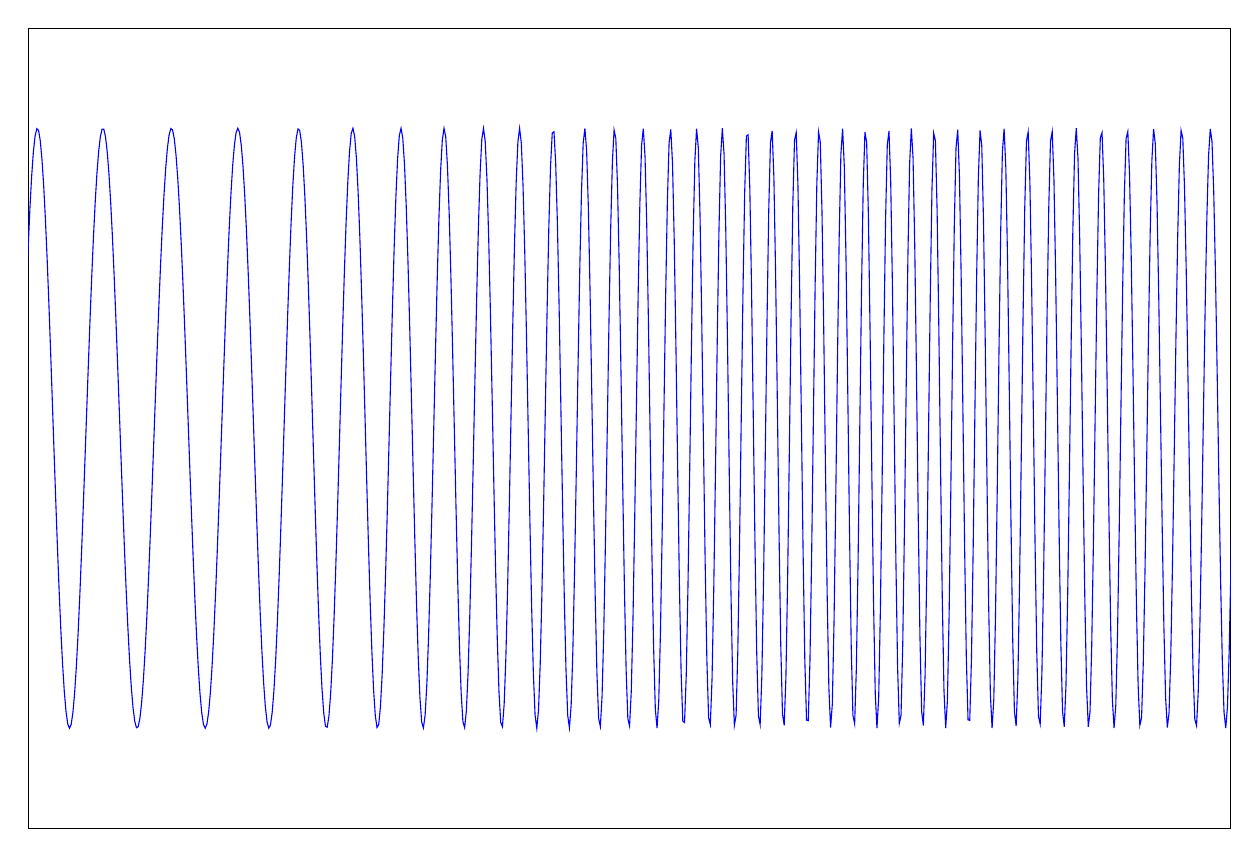
\begin{tikzpicture}

\begin{axis}[%
width=6.01339838214984in,
height=4in,
scale only axis,
xmin=100,
xmax=800,
ymin=-0.4,
ymax=0.4,
ticks=none,
xticklabels={\empty}
]
\addplot [color=blue,solid,forget plot]
  table[row sep=crcr]{1	-0.285595208280874\\
2	-0.253510297549853\\
3	-0.205505183025438\\
4	-0.144785975300412\\
5	-0.0752888494582544\\
6	-0.00141531961632902\\
7	0.0722518657532913\\
8	0.141233844187643\\
9	0.201424284382721\\
10	0.249325963285151\\
11	0.282242421147897\\
12	0.298415197442985\\
13	0.297100881022908\\
14	0.278586063095336\\
15	0.24414202319198\\
16	0.195924392552344\\
17	0.136825947531264\\
18	0.0702929520504031\\
19	0.000117004505442704\\
20	-0.069784888593991\\
21	-0.13558928500611\\
22	-0.193772304440653\\
23	-0.241291961919609\\
24	-0.275737987448987\\
25	-0.295442496836185\\
26	-0.299547320851793\\
27	-0.288026323027502\\
28	-0.261663499298576\\
29	-0.221989928261676\\
30	-0.171184621269982\\
31	-0.111945922818421\\
32	-0.0473412757124193\\
33	0.0193561384937714\\
34	0.0848351497748264\\
35	0.14591023538467\\
36	0.199673175262993\\
37	0.243625852107062\\
38	0.275788590879548\\
39	0.294779900322065\\
40	0.299865060222971\\
41	0.290972608819381\\
42	0.268679345674163\\
43	0.23416590577605\\
44	0.189146220558304\\
45	0.135775214065471\\
46	0.0765398548036093\\
47	0.0141391775542496\\
48	-0.0486408994971128\\
49	-0.109052199478333\\
50	-0.164502905814273\\
51	-0.212665265263427\\
52	-0.25156818590584\\
53	-0.279671402273405\\
54	-0.295918834623024\\
55	-0.299769770510863\\
56	-0.29120749846276\\
57	-0.270725983229342\\
58	-0.239296052218881\\
59	-0.198313331710237\\
60	-0.149530804755572\\
61	-0.0949793430797008\\
62	-0.0368798831084847\\
63	0.0224489308873375\\
64	0.0806838211459638\\
65	0.135587010397414\\
66	0.185090049256262\\
67	0.227368376632805\\
68	0.260904149855449\\
69	0.284535444600662\\
70	0.297490528844391\\
71	0.299406534448312\\
72	0.290332460503239\\
73	0.270717022019245\\
74	0.241382386529876\\
75	0.203485303442285\\
76	0.1584675138626\\
77	0.107997623257591\\
78	0.0539068205673976\\
79	-0.001879066151757\\
80	-0.0574086737819805\\
81	-0.110772938066105\\
82	-0.160169381268816\\
83	-0.203960800876073\\
84	-0.240726587997529\\
85	-0.269305230485968\\
86	-0.28882691353027\\
87	-0.298735505880531\\
88	-0.298799599491934\\
89	-0.289112641582938\\
90	-0.270082549317947\\
91	-0.242411518390084\\
92	-0.207067019162777\\
93	-0.165245210983654\\
94	-0.118328191909728\\
95	-0.0678366344120622\\
96	-0.0153794364661369\\
97	0.0373979575729322\\
98	0.0888649386150362\\
99	0.137455264016304\\
100	0.181713303231999\\
101	0.220335718129112\\
102	0.252207484171325\\
103	0.276431368368213\\
104	0.292350205895709\\
105	0.299561552230889\\
106	0.297924524311811\\
107	0.287558875803663\\
108	0.268836571731209\\
109	0.242366330916252\\
110	0.208971786028642\\
111	0.169664066666762\\
112	0.125609737717871\\
113	0.0780951212364819\\
114	0.0284880940875963\\
115	-0.0218015145779948\\
116	-0.0713618016682545\\
117	-0.118817849793494\\
118	-0.162868931441767\\
119	-0.202322903881226\\
120	-0.236126945842686\\
121	-0.263393910161863\\
122	-0.283423703997746\\
123	-0.295719255897642\\
124	-0.299996782689768\\
125	-0.296190224833412\\
126	-0.284449872500148\\
127	-0.265135352550461\\
128	-0.238803285302543\\
129	-0.20619004651145\\
130	-0.168190181676903\\
131	-0.125831114513424\\
132	-0.0802448675058695\\
133	-0.0326375687505787\\
134	0.0157424448649155\\
135	0.0636371028346193\\
136	0.109810834263407\\
137	0.153081763347951\\
138	0.192351114092843\\
139	0.226630130773323\\
140	0.255063895051136\\
141	0.276951507763545\\
142	0.291762200889264\\
143	0.29914705056557\\
144	0.298946072673248\\
145	0.291190595815079\\
146	0.276100919877457\\
147	0.254079379256429\\
148	0.225699035849931\\
149	0.191688325822327\\
150	0.152912073929239\\
151	0.110349368042651\\
152	0.0650688529608659\\
153	0.0182020553765647\\
154	-0.0290846098550758\\
155	-0.0756184788785265\\
156	-0.120249242398818\\
157	-0.161876840165418\\
158	-0.199477995396104\\
159	-0.232130774897552\\
160	-0.259036610677235\\
161	-0.279539280951591\\
162	-0.293140421182422\\
163	-0.299511217489579\\
164	-0.298500023643356\\
165	-0.290135736934584\\
166	-0.274626865484744\\
167	-0.252356317935307\\
168	-0.223872043836947\\
169	-0.189873747390278\\
170	-0.151195986467414\\
171	-0.108788051188012\\
172	-0.0636910899770671\\
173	-0.017013014428251\\
174	0.0300982339303417\\
175	0.0764824328666274\\
176	0.12099519719633\\
177	0.162535806471293\\
178	0.200074087483127\\
179	0.232675714510982\\
180	0.259525322647908\\
181	0.279946875690781\\
182	0.293420789142696\\
183	0.299597379718135\\
184	0.298306293957365\\
185	0.289561658525991\\
186	0.273562791658217\\
187	0.250690416983003\\
188	0.221498425494467\\
189	0.186701336439447\\
190	0.147157711079671\\
191	0.103849872321657\\
192	0.0578603758022422\\
193	0.010345761965286\\
194	-0.0374918081106311\\
195	-0.0844343697716421\\
196	-0.129278715063398\\
197	-0.170866955944763\\
198	-0.208116336374449\\
199	-0.240047542962032\\
200	-0.265810785618845\\
201	-0.284708959337987\\
202	-0.29621725547892\\
203	-0.299998664928899\\
204	-0.295914904997534\\
205	-0.284032405249307\\
206	-0.264623102661193\\
207	-0.238159921126892\\
208	-0.205306941715369\\
209	-0.166904405258037\\
210	-0.123948824595784\\
211	-0.0775686168448057\\
212	-0.0289957928903414\\
213	0.0204656413769801\\
214	0.0694738131860893\\
215	0.11668479315909\\
216	0.160789171161621\\
217	0.200548433381286\\
218	0.234830152163092\\
219	0.262641001359958\\
220	0.283156637579555\\
221	0.295747542144637\\
222	0.299999999616356\\
223	0.295731495342615\\
224	0.282999945013196\\
225	0.262106321160454\\
226	0.233590411787423\\
227	0.198219630992345\\
228	0.156970996131207\\
229	0.11100658573849\\
230	0.0616429916986057\\
231	0.0103154723028537\\
232	-0.0414623060145043\\
233	-0.0921418871817618\\
234	-0.14018581345702\\
235	-0.184114281302165\\
236	-0.222551286597922\\
237	-0.254268841528363\\
238	-0.278227847458412\\
239	-0.293614253458537\\
240	-0.299869219771277\\
241	-0.296712139184758\\
242	-0.284155545276443\\
243	-0.262511151702509\\
244	-0.232386516552009\\
245	-0.194672104284611\\
246	-0.150518817633045\\
247	-0.101306384586072\\
248	-0.0486033017083857\\
249	0.00588065560551389\\
250	0.0603480535473552\\
251	0.112971985102442\\
252	0.161957029679266\\
253	0.205601021300207\\
254	0.242355542026221\\
255	0.270883005531492\\
256	0.290108215557755\\
257	0.299262379139632\\
258	0.297917726373476\\
259	0.286011135770071\\
260	0.263855482752293\\
261	0.232137811584725\\
262	0.191903868016876\\
263	0.144529008496368\\
264	0.0916760068130586\\
265	0.035240793148318\\
266	-0.0227123351542362\\
267	-0.0800240171851465\\
268	-0.134519207915123\\
269	-0.184089840212138\\
270	-0.226777709751782\\
271	-0.260854361580484\\
272	-0.284894713759858\\
273	-0.297841238151342\\
274	-0.299055736127374\\
275	-0.288356097931891\\
276	-0.266035913083793\\
277	-0.232865394408253\\
278	-0.190072772959624\\
279	-0.13930609268932\\
280	-0.0825761545786212\\
281	-0.0221821981780085\\
282	0.0393772710611969\\
283	0.0995053347443277\\
284	0.155615347757318\\
285	0.205243066420068\\
286	0.246157445060477\\
287	0.276465136021935\\
288	0.294703749400155\\
289	0.29991917672239\\
290	0.291722761729442\\
291	0.270324805234553\\
292	0.23654180234047\\
293	0.191775900409514\\
294	0.137966295481781\\
295	0.0775136037558594\\
296	0.0131795953911683\\
297	-0.0520340038568193\\
298	-0.11502271932763\\
299	-0.172726568211706\\
300	-0.222280542328708\\
301	-0.26116101385328\\
302	-0.287320556246062\\
303	-0.299303856169009\\
304	-0.296337964855043\\
305	-0.278391096927019\\
306	-0.246195507879147\\
307	-0.201231623710862\\
308	-0.145672492025576\\
309	-0.0822896885942785\\
310	-0.0143239461782733\\
311	0.0546741393732702\\
312	0.121026046254938\\
313	0.181120986312078\\
314	0.231615121275208\\
315	0.269623419968268\\
316	0.292893064798576\\
317	0.299947764691238\\
318	0.290193423852572\\
319	0.263977333045855\\
320	0.222595335262535\\
321	0.168244174745096\\
322	0.103919334840178\\
323	0.0332619422971816\\
324	-0.0396384243953782\\
325	-0.110475139243916\\
326	-0.174977635243542\\
327	-0.22917168921068\\
328	-0.269631131631771\\
329	-0.293704916919936\\
330	-0.299704181443585\\
331	-0.287035638183314\\
332	-0.256270368459667\\
333	-0.209140664533534\\
334	-0.148461876138622\\
335	-0.0779809817620263\\
336	-0.00215855373391161\\
337	0.0741044081404492\\
338	0.145778975277096\\
339	0.208040810924948\\
340	0.256601005027981\\
341	0.288012478215635\\
342	0.299929700380377\\
343	0.291301559599119\\
344	0.262480868820731\\
345	0.215239055635324\\
346	0.152680774096477\\
347	0.0790601314780805\\
348	-0.000492524277260993\\
349	-0.0803172782996974\\
350	-0.154622536628782\\
351	-0.217906901980012\\
352	-0.265374590007632\\
353	-0.2933128428866\\
354	-0.299401056863635\\
355	-0.282925018371842\\
356	-0.244875615137067\\
357	-0.187919337773666\\
358	-0.116237314023994\\
359	-0.0352398648938394\\
360	0.0488261343078818\\
361	0.129350300539103\\
362	0.199877528079036\\
363	0.254632344876836\\
364	0.289006176004452\\
365	0.299965763737038\\
366	0.286345467652046\\
367	0.248994056997983\\
368	0.190757460233337\\
369	0.116292010290346\\
370	0.031717026427622\\
371	-0.0558700693906719\\
372	-0.13897975659647\\
373	-0.210370507341061\\
374	-0.263688820066318\\
375	-0.294052389008419\\
376	-0.298521921965321\\
377	-0.276414525907801\\
378	-0.229423719813437\\
379	-0.161527182231283\\
380	-0.0786820463176318\\
381	0.0116726750264463\\
382	0.101267924082746\\
383	0.181755662988312\\
384	0.245492067428361\\
385	0.286279470361781\\
386	0.299994165461619\\
387	0.285034809833423\\
388	0.242540626503874\\
389	0.176348883242863\\
390	0.0926855428108162\\
391	-0.000390667891873555\\
392	-0.0937447940994565\\
393	-0.178054384178177\\
394	-0.244745372783741\\
395	-0.28688132042978\\
396	-0.299912728414839\\
397	-0.282203434352741\\
398	-0.235270649969198\\
399	-0.163702501957884\\
400	-0.0747495151321571\\
401	0.0223788647111988\\
402	0.117448511147523\\
403	0.200273589417248\\
404	0.261817028740784\\
405	0.295199323553006\\
406	0.29650135292249\\
407	0.26526476301053\\
408	0.204623043083826\\
409	0.121035056443441\\
410	0.023636568341961\\
411	-0.0767304951376784\\
412	-0.16871180743785\\
413	-0.241728193526827\\
414	-0.287211351585398\\
415	-0.299642002025287\\
416	-0.277261794603242\\
417	-0.222363487064852\\
418	-0.141110107415198\\
419	-0.0428881637753088\\
420	0.0607436847676697\\
421	0.15739751204075\\
422	0.235337384016927\\
423	0.284922577259561\\
424	0.299833861094939\\
425	0.277923643573813\\
426	0.221571350247205\\
427	0.137482814492136\\
428	0.0359402844702375\\
429	-0.0704202459656998\\
430	-0.16816420733111\\
431	-0.244757681821057\\
432	-0.290196245784553\\
433	-0.298349804721451\\
434	-0.267838694917289\\
435	-0.202310895659196\\
436	-0.110064463876929\\
437	-0.00304430794538969\\
438	0.104672756020949\\
439	0.198717572783744\\
440	0.266354816471778\\
441	0.298237084298636\\
442	0.289742196642437\\
443	0.241697295461062\\
444	0.160370935839148\\
445	0.0567118108333659\\
446	-0.0550827194020229\\
447	-0.159487949420965\\
448	-0.241806997955105\\
449	-0.290261498027482\\
450	-0.297718125863585\\
451	-0.262792998103036\\
452	-0.190156679907726\\
453	-0.0899722807937952\\
454	0.0234768888066393\\
455	0.133792986671107\\
456	0.224826244644429\\
457	0.283055937321539\\
458	0.299636991996929\\
459	0.271797657542348\\
460	0.203360615773877\\
461	0.104284651069886\\
462	-0.010730881420476\\
463	-0.124392379195041\\
464	-0.21940170951329\\
465	-0.281103807882911\\
466	-0.299785351349044\\
467	-0.272258935433183\\
468	-0.20246709231482\\
469	-0.100985765489665\\
470	0.0165236160238992\\
471	0.131696496147254\\
472	0.226325756824505\\
473	0.285257056593615\\
474	0.298856485350174\\
475	0.264643025794977\\
476	0.187801223074821\\
477	0.0804629422798138\\
478	-0.0401553287961194\\
479	-0.154483090473244\\
480	-0.243766936344381\\
481	-0.293169602211196\\
482	-0.294281700938943\\
483	-0.246614147248914\\
484	-0.157797711984513\\
485	-0.042425790096999\\
486	0.0802963312786549\\
487	0.189725680388839\\
488	0.267259044104937\\
489	0.299527502943133\\
490	0.280754666310283\\
491	0.213854441329321\\
492	0.110050814177882\\
493	-0.0129471244483937\\
494	-0.133929150586541\\
495	-0.231831080106852\\
496	-0.289420249826491\\
497	-0.296371797579871\\
498	-0.251179658225408\\
499	-0.16153913453556\\
500	-0.0431011828120528\\
501	0.0832127894696841\\
502	0.194883948196787\\
503	0.271816459909066\\
504	0.299986833837163\\
505	0.274053977302461\\
506	0.198435202607527\\
507	0.0866220217007219\\
508	-0.04117316085009\\
509	-0.161639450533733\\
510	-0.252615854549268\\
511	-0.297192333828885\\
512	-0.286900408827119\\
513	-0.223383044466116\\
514	-0.118204429526218\\
515	0.00919836955448768\\
516	0.135070471547076\\
517	0.235757953583325\\
518	0.292170504811743\\
519	0.29344288048565\\
520	0.239085319313917\\
521	0.13918721713479\\
522	0.0126023923980989\\
523	-0.116569535245951\\
524	-0.223556830960511\\
525	-0.287679248043579\\
526	-0.296383066186758\\
527	-0.247753211190645\\
528	-0.150989845785789\\
529	-0.0247248564906396\\
530	0.106525641505867\\
531	0.217105354847289\\
532	0.285243547629272\\
533	0.297375877078354\\
534	0.250896043824635\\
535	0.154770380011779\\
536	0.0278628280242492\\
537	-0.104728368151223\\
538	-0.216618629816227\\
539	-0.285397219071277\\
540	-0.297148815727849\\
541	-0.249317625081584\\
542	-0.151315069900019\\
543	-0.0227190391276406\\
544	0.110601644620501\\
545	0.221677531847344\\
546	0.287904782180192\\
547	0.295677032280967\\
548	0.243227139643366\\
549	0.141076108713248\\
550	0.00996913495147715\\
551	-0.123306227801633\\
552	-0.231383067861083\\
553	-0.291946950696199\\
554	-0.292374755194148\\
555	-0.232409465489701\\
556	-0.124295297114405\\
557	0.00968144775813793\\
558	0.141760562253989\\
559	0.244453901079744\\
560	0.29628063136397\\
561	0.286291716825479\\
562	0.216423889359842\\
563	0.101168669700366\\
564	-0.0353986245336722\\
565	-0.164628038231566\\
566	-0.259303889740126\\
567	-0.299392949275762\\
568	-0.276313855908423\\
569	-0.194811200544907\\
570	-0.0720173656514589\\
571	0.0661208746750308\\
572	0.190311378453105\\
573	0.274130928719369\\
574	0.299665230301542\\
575	0.261366391413207\\
576	0.167290861972415\\
577	0.037435010915994\\
578	-0.100494387752634\\
579	-0.216984244238631\\
580	-0.287036726914771\\
581	-0.295552200163492\\
582	-0.240609858488294\\
583	-0.133927470210491\\
584	0.00161459486136121\\
585	0.136866704790022\\
586	0.242676625859029\\
587	0.296182076809411\\
588	0.285768264246191\\
589	0.213611041415033\\
590	0.0952439284862731\\
591	-0.0437699948196122\\
592	-0.173351359623276\\
593	-0.265414861556082\\
594	-0.299966439176232\\
595	-0.269460734529791\\
596	-0.180465391274613\\
597	-0.0522613873128851\\
598	0.0873253284693463\\
599	0.207961184600276\\
600	0.283401146693658\\
601	0.297207582369778\\
602	0.246343008390564\\
603	0.141848611515797\\
604	0.00645473888310909\\
605	-0.130360803024087\\
606	-0.238792289267114\\
607	-0.2952042907773\\
608	-0.287289955078485\\
609	-0.216761579158149\\
610	-0.0989836790514605\\
611	0.0403735585256843\\
612	0.170931247228806\\
613	0.264227728311527\\
614	0.299926683969343\\
615	0.270251790822604\\
616	0.181679918592732\\
617	0.0535241500924046\\
618	-0.0862824781099003\\
619	-0.207280439745413\\
620	-0.283123257051286\\
621	-0.297314285974336\\
622	-0.246790890725025\\
623	-0.142577728696619\\
624	-0.00737143871141172\\
625	0.129411738195359\\
626	0.238042188098689\\
627	0.294939724514919\\
628	0.287787015365418\\
629	0.218185270651664\\
630	0.101281668134351\\
631	-0.0375419906676293\\
632	-0.168191893565626\\
633	-0.262391279113749\\
634	-0.299797481116763\\
635	-0.272383595266849\\
636	-0.186142969627382\\
637	-0.0597583787649564\\
638	0.0794641797059386\\
639	0.201507578820864\\
640	0.28011814228711\\
641	0.298444852442424\\
642	0.2526330997151\\
643	0.152610184675564\\
644	0.0199082541449797\\
645	-0.116992259354992\\
646	-0.228786630646371\\
647	-0.291617336757813\\
648	-0.292150539683282\\
649	-0.23038004486952\\
650	-0.119574442279418\\
651	0.0166030380265682\\
652	0.149170241783501\\
653	0.250003432810102\\
654	0.297797046841662\\
655	0.282543749504368\\
656	0.207596993036786\\
657	0.0888980179515314\\
658	-0.048447849681888\\
659	-0.175503162007355\\
660	-0.265601046901934\\
661	-0.299929850700187\\
662	-0.27143230229811\\
663	-0.186216791981324\\
664	-0.0622072794354522\\
665	0.0746617876740369\\
666	0.195890286415183\\
667	0.276349054306098\\
668	0.299470844025822\\
669	0.260626696117335\\
670	0.168006850918365\\
671	0.040849090343441\\
672	-0.0945934668550894\\
673	-0.210492337071563\\
674	-0.283159783764452\\
675	-0.297866922668256\\
676	-0.251788363485834\\
677	-0.154493158973505\\
678	-0.0259095396135969\\
679	0.107794338799882\\
680	0.219554464127986\\
681	0.286884462944847\\
682	0.296372247512726\\
683	0.246306099205839\\
684	0.146925495828964\\
685	0.0182759187549432\\
686	-0.113873211236181\\
687	-0.223208429950659\\
688	-0.288104972016227\\
689	-0.295872961625849\\
690	-0.245189421291627\\
691	-0.146260240481763\\
692	-0.0187112124909773\\
693	0.112346061319402\\
694	0.221276881567441\\
695	0.286930263393767\\
696	0.296713327800025\\
697	0.248954855658388\\
698	0.153125036151759\\
699	0.0279008742444503\\
700	-0.10251736443956\\
701	-0.213104009590423\\
702	-0.28280417102563\\
703	-0.298510241571207\\
704	-0.257474054887951\\
705	-0.167721475543947\\
706	-0.0464231386969366\\
707	0.0834377255019658\\
708	0.197445147901325\\
709	0.274338725855494\\
710	0.299948699027898\\
711	0.26975526210536\\
712	0.189620147656052\\
713	0.0745867081234093\\
714	-0.0539960812089844\\
715	-0.172466774202553\\
716	-0.259209430606112\\
717	-0.298573278583118\\
718	-0.28364807297833\\
719	-0.217412424152736\\
720	-0.112077626897469\\
721	0.0132208511428238\\
722	0.135938246543154\\
723	0.23418956918408\\
724	0.290636498956552\\
725	0.295504997817756\\
726	0.248216487915293\\
727	0.157372370285797\\
728	0.0391275368992834\\
729	-0.0857298862356003\\
730	-0.195456952079557\\
731	-0.271137851380898\\
732	-0.299912771859265\\
733	-0.277108594587776\\
734	-0.206928681781768\\
735	-0.101614360464022\\
736	0.0207463599538509\\
737	0.139361879618787\\
738	0.234280111335763\\
739	0.289726578914697\\
740	0.296682602594477\\
741	0.254290201480942\\
742	0.169876546994663\\
743	0.057625135073131\\
744	-0.0638565020933886\\
745	-0.174648092791771\\
746	-0.256782885633684\\
747	-0.29713391918073\\
748	-0.289461747737765\\
749	-0.235313254693452\\
750	-0.143654630016344\\
751	-0.0293275423515587\\
752	0.0893974298427927\\
753	0.193760646933359\\
754	0.267470953287523\\
755	0.299216340238776\\
756	0.284346644197839\\
757	0.225487369501894\\
758	0.13201657557126\\
759	0.0185142403991753\\
760	-0.0975519584277521\\
761	-0.198531758108257\\
762	-0.269267498036221\\
763	-0.299335963310913\\
764	-0.284531174212982\\
765	-0.227386300487235\\
766	-0.136682516698481\\
767	-0.0260446323341207\\
768	0.0881449382155137\\
769	0.189189483337788\\
770	0.262512331013531\\
771	0.297729058617527\\
772	0.290068269039223\\
773	0.240954855651556\\
774	0.157695753593625\\
775	0.0523380576390153\\
776	-0.0601156008083066\\
777	-0.163865053541938\\
778	-0.244531271673896\\
779	-0.291125106078438\\
780	-0.297500712576847\\
781	-0.263108477489274\\
782	-0.192964792863688\\
783	-0.0968658232330671\\
784	0.01202586809398\\
785	0.119012764572339\\
786	0.209854033109986\\
787	0.272647178372863\\
788	0.299353738239017\\
789	0.286778834961733\\
790	0.236892945377355\\
791	0.156474177425435\\
792	0.056138355147056\\
793	-0.0510992045840251\\
794	-0.151531500556216\\
795	-0.232511432045028\\
796	-0.284024153862855\\
797	-0.299888096829487\\
798	-0.278446292095802\\
799	-0.222678369878723\\
800	-0.139738017328908\\
801	-0.0399912670868967\\
802	0.0643107688435686\\
803	0.160551735736504\\
804	0.23727282334909\\
805	0.285515862514712\\
806	0.299832659471637\\
807	0.278852150519592\\
808	0.225353404274181\\
809	0.145852513120663\\
810	0.0497677663868334\\
811	-0.0517262065318287\\
812	-0.147013248482368\\
813	-0.225363738658063\\
814	-0.278124972159304\\
815	-0.299644579171363\\
816	-0.287832924810296\\
817	-0.244314530120716\\
818	-0.174166139566628\\
819	-0.08528466251498\\
820	0.0125330891488027\\
821	0.108689029314392\\
822	0.192936277404792\\
823	0.256460411257117\\
824	0.29277725921127\\
825	0.298359149006631\\
826	0.272933809739159\\
827	0.219436681288671\\
828	0.143634160132836\\
829	0.0534684647073409\\
830	-0.0417988869131414\\
831	-0.13255084799784\\
832	-0.209784976492794\\
833	-0.265992795687498\\
834	-0.295864528624831\\
835	-0.296756298886339\\
836	-0.268882988622483\\
837	-0.215228330117251\\
838	-0.14119157140195\\
839	-0.0540145367668146\\
840	0.0379480743821225\\
841	0.126040250291428\\
842	0.202118844754842\\
843	0.259294450090257\\
844	0.292533284857118\\
845	0.299070210083668\\
846	0.278602548525\\
847	0.233255689409121\\
848	0.16733246867352\\
849	0.0868771362414365\\
850	-0.000900205831283553\\
851	-0.088282610248676\\
852	-0.167727937286009\\
853	-0.232513210764461\\
854	-0.277287752180897\\
855	-0.298491513504597\\
856	-0.294608549281085\\
857	-0.266240914446152\\
858	-0.216004031593223\\
859	-0.148259387098164\\
860	-0.0687131074539479\\
861	0.0160813884873871\\
862	0.0992724766063103\\
863	0.174264900145805\\
864	0.235235350757232\\
865	0.277569821594141\\
866	0.298191566222121\\
867	0.295758579283239\\
868	0.270720688505003\\
869	0.225237670028718\\
870	0.162970381448705\\
871	0.0887659801708288\\
872	0.00826525970910534\\
873	-0.0725354023138662\\
874	-0.147733211060411\\
875	-0.211945827698011\\
876	-0.260685817370283\\
877	-0.290657834482044\\
878	-0.299960503466183\\
879	-0.288182661364066\\
880	-0.256391636040339\\
881	-0.207018949584036\\
882	-0.143655732385051\\
883	-0.0707757774199975\\
884	0.00659175655959438\\
885	0.0832156512178885\\
886	0.154017062756357\\
887	0.214401376491945\\
888	0.260546471360362\\
889	0.289630323555509\\
890	0.299985717747602\\
891	0.29117519458571\\
892	0.263984859096628\\
893	0.220340939825823\\
894	0.163157698542467\\
895	0.0961291799785632\\
896	0.0234801672908803\\
897	-0.0503065428313789\\
898	-0.120768846209033\\
899	-0.183732856435477\\
900	-0.235553640105732\\
901	-0.27331595896504\\
902	-0.294984873512595\\
903	-0.299499544786984\\
904	-0.286807242207106\\
905	-0.257838195918448\\
906	-0.214425311885522\\
907	-0.159175717028861\\
908	-0.0953034784715779\\
909	-0.0264345474441199\\
910	0.0436040377250387\\
911	0.110998401130597\\
912	0.172153684462543\\
913	0.22388072720309\\
914	0.263554381901383\\
915	0.289236268021882\\
916	0.299757029351503\\
917	0.29475555028696\\
918	0.274674969691393\\
919	0.240717582038308\\
920	0.194762725208247\\
921	0.139253434284682\\
922	0.0770589264300631\\
923	0.0113208339926333\\
924	-0.0547084928761739\\
925	-0.117827327122644\\
926	-0.175037704049291\\
927	-0.22368331411896\\
928	-0.261566200250691\\
929	-0.287037628760033\\
930	-0.299059965344725\\
931	-0.297237914247493\\
932	-0.281818993161789\\
933	-0.253664548087873\\
934	-0.214193899805201\\
935	-0.165305306796737\\
936	-0.10927829095233\\
937	-0.0486624782369447\\
938	0.0138415538163849\\
939	0.0755038540960608\\
940	0.133683707755096\\
941	0.185940284126884\\
942	0.230130922246834\\
943	0.264493401923475\\
944	0.287709409408262\\
945	0.298947336439284\\
946	0.29788350593095\\
947	0.284701855156063\\
948	0.260072989971292\\
949	0.225114318555749\\
950	0.181333653367559\\
951	0.130559215318252\\
952	0.0748593712277649\\
953	0.0164556780769016\\
954	-0.0423671042923962\\
955	-0.0993504301859911\\
956	-0.152347408916222\\
957	-0.199401179615425\\
958	-0.238813546278516\\
959	-0.269201693568046\\
960	-0.289541352642681\\
961	-0.299195365519705\\
962	-0.297927182807347\\
963	-0.285899400993223\\
964	-0.263657981896518\\
965	-0.232103281074273\\
966	-0.192449429729963\\
967	-0.14617395515032\\
968	-0.0949597805869903\\
969	-0.0406319129397103\\
970	0.0149087948800098\\
971	0.0697524277526237\\
972	0.122045047751994\\
973	0.170049860102552\\
974	0.21220260139801\\
975	0.247159522444127\\
976	0.273836654445178\\
977	0.291439390537547\\
978	0.29948177211002\\
979	0.297795228523788\\
980	0.286526868097609\\
981	0.266127746971499\\
982	0.237331841462744\\
983	0.201126711059423\\
984	0.15871705721241\\
985	0.111482553262691\\
986	0.0609314406027932\\
987	0.00865145465050592\\
988	-0.0437403378755243\\
989	-0.0946472393254536\\
990	-0.142540683365865\\
991	-0.186004698862109\\
992	-0.223775865373198\\
993	-0.254777728993216\\
994	-0.27814884788493\\
995	-0.293263852458713\\
996	-0.299747128843449\\
997	-0.297478959341345\\
998	-0.286594173586278\\
999	-0.267473573252297\\
1000	-0.240728586142558\\
1001	-0.207179777818984\\
1002	-0.167829996914134\\
1003	-0.123833051040758\\
1004	-0.0764589018398553\\
1005	-0.0270564290759307\\
1006	0.0229851554354352\\
1007	0.0722751622983427\\
1008	0.119459493280947\\
1009	0.163256924455059\\
1010	0.202492682168576\\
1011	0.236128489626879\\
1012	0.263288378816924\\
1013	0.283279693366065\\
1014	0.295608848879328\\
1015	0.299991564370957\\
1016	0.296357427753099\\
1017	0.28484880617489\\
1018	0.265814254773011\\
1019	0.239796711815655\\
1020	0.207516891351565\\
1021	0.169852393772116\\
1022	0.127813148031863\\
1023	0.0825138749916978\\
1024	0.0351443182570689\\
1025	-0.0130619737158312\\
1026	-0.0608595128468759\\
1027	-0.107022584494808\\
1028	-0.150376029655909\\
1029	-0.189824356244214\\
1030	-0.224378494480938\\
1031	-0.253179581210981\\
1032	-0.275519240491381\\
1033	-0.290855920836337\\
1034	-0.298826950705632\\
1035	-0.299256080714512\\
1036	-0.292156391107539\\
1037	-0.277728553755201\\
1038	-0.256354546843315\\
1039	-0.22858702517103\\
1040	-0.195134647336616\\
1041	-0.156843751055813\\
1042	-0.114676847613045\\
1043	-0.0696884744385525\\
1044	-0.0229989997759518\\
1045	0.0242329856399205\\
1046	0.0708390287159055\\
1047	0.115669253523727\\
1048	0.157620211658827\\
1049	0.195661493564768\\
1050	0.228860483876758\\
1051	0.256404690197774\\
1052	0.277621133352837\\
1053	0.291992356766069\\
1054	0.299168691586334\\
1055	0.298976500826589\\
1056	0.291422218194466\\
1057	0.27669209349482\\
1058	0.255147654423518\\
1059	0.227316992162462\\
1060	0.193882073361118\\
1061	0.155662371821634\\
1062	0.113595197570212\\
1063	0.0687131771798911\\
1064	0.0221194055693098\\
1065	-0.0250391554194637\\
1066	-0.0715994137863434\\
1067	-0.116410372542707\\
1068	-0.158361181484284\\
1069	-0.196408353563317\\
1070	-0.229601498444925\\
1071	-0.257106955035577\\
1072	-0.278228748138885\\
1073	-0.292426351143133\\
1074	-0.299328805731999\\
1075	-0.298744829686145\\
1076	-0.290668633341467\\
1077	-0.275281262362427\\
1078	-0.25294738717554\\
1079	-0.224207565515466\\
1080	-0.18976611177283\\
1081	-0.150474812829542\\
1082	-0.107312832430513\\
1083	-0.06136324247825\\
1084	-0.0137867076409753\\
1085	0.0342070728647509\\
1086	0.0813894975400074\\
1087	0.126544049600347\\
1088	0.168497384770622\\
1089	0.2061497484612\\
1090	0.238503951509926\\
1091	0.264692152805535\\
1092	0.283999734938296\\
1093	0.295885615185388\\
1094	0.299998407916185\\
1095	0.296187944673433\\
1096	0.284511763136718\\
1097	0.265236293865961\\
1098	0.238832601717517\\
1099	0.20596667435375\\
1100	0.167484390254048\\
1101	0.124391439743397\\
1102	0.0778286113151798\\
1103	0.0290429883186512\\
1104	-0.0206442756987596\\
1105	-0.0698728245917191\\
1106	-0.117279738145456\\
1107	-0.161536995518585\\
1108	-0.201388765988116\\
1109	-0.235687502497551\\
1110	-0.263427813158294\\
1111	-0.283777113219807\\
1112	-0.296102115650335\\
1113	-0.299990302129652\\
1114	-0.295265626995036\\
1115	-0.28199784272237\\
1116	-0.260504994323094\\
1117	-0.231348808252539\\
1118	-0.195322895002913\\
1119	-0.153433888770492\\
1120	-0.106875857126833\\
1121	-0.0569985227376798\\
1122	-0.00527004175615998\\
1123	0.0467647266989967\\
1124	0.0975293548639875\\
1125	0.145463133779596\\
1126	0.189069148538336\\
1127	0.226961697354133\\
1128	0.257911572227796\\
1129	0.280887724531955\\
1130	0.295093890466829\\
1131	0.299998850024116\\
1132	0.295359138415341\\
1133	0.281233218934027\\
1134	0.257986357434618\\
1135	0.226285705977772\\
1136	0.187085400139896\\
1137	0.141601793047155\\
1138	0.0912792801269644\\
1139	0.0377475016118753\\
1140	-0.0172289660762266\\
1141	-0.0718070152891353\\
1142	-0.124125822110379\\
1143	-0.17237015673689\\
1144	-0.214834100463298\\
1145	-0.249982969602582\\
1146	-0.276511207110342\\
1147	-0.293394040282291\\
1148	-0.299930821186321\\
1149	-0.295778166332067\\
1150	-0.280971291380245\\
1151	-0.255932290301654\\
1152	-0.221464527986866\\
1153	-0.178732789488264\\
1154	-0.129229343521118\\
1155	-0.0747266156676568\\
1156	-0.0172177088275088\\
1157	0.0411534658027802\\
1158	0.0981701961113519\\
1159	0.15162643548436\\
1160	0.199412701217833\\
1161	0.239601129994474\\
1162	0.270526284052067\\
1163	0.290858299890501\\
1164	0.299665108068404\\
1165	0.296460731560441\\
1166	0.281237089347778\\
1167	0.254477283354359\\
1168	0.217149016220646\\
1169	0.170677554234711\\
1170	0.116898487703881\\
1171	0.0579914186941531\\
1172	-0.00360341230302898\\
1173	-0.0652827022040143\\
1174	-0.124388232818161\\
1175	-0.178321301420518\\
1176	-0.224658640465748\\
1177	-0.26126471310848\\
1178	-0.286395165531796\\
1179	-0.298786344993536\\
1180	-0.297726164418545\\
1181	-0.28310220988385\\
1182	-0.25542383435257\\
1183	-0.215816035209923\\
1184	-0.165984138200133\\
1185	-0.108149658606841\\
1186	-0.0449591244019805\\
1187	0.0206309398223591\\
1188	0.0854883256709166\\
1189	0.146453007571251\\
1190	0.200491834101543\\
1191	0.244852608860055\\
1192	0.277209756147601\\
1193	0.295793776894705\\
1194	0.299497116668746\\
1195	0.287949897171795\\
1196	0.261560190597039\\
1197	0.221515104890682\\
1198	0.169740836933007\\
1199	0.108821958024962\\
1200	0.0418824212202293\\
1201	-0.0275669923282235\\
1202	-0.0958079654308469\\
1203	-0.159111997286077\\
1204	-0.213945656265035\\
1205	-0.257172576427233\\
1206	-0.286240622202422\\
1207	-0.299342870168517\\
1208	-0.295541957480483\\
1209	-0.274848918112096\\
1210	-0.238249824519507\\
1211	-0.187676285770035\\
1212	-0.125918995741158\\
1213	-0.0564869132953762\\
1214	0.0165819013751292\\
1215	0.0889484842420826\\
1216	0.156227976760602\\
1217	0.214256897538076\\
1218	0.259356573832085\\
1219	0.288576006473673\\
1220	0.299897853305312\\
1221	0.292392709514581\\
1222	0.266309416505895\\
1223	0.223092649677106\\
1224	0.165323352478762\\
1225	0.0965824647615312\\
1226	0.0212435458272554\\
1227	-0.0557950167876149\\
1228	-0.129422848509634\\
1229	-0.194656212837226\\
1230	-0.246980351421584\\
1231	-0.282672040871995\\
1232	-0.299079009850082\\
1233	-0.294834672166863\\
1234	-0.269990099245131\\
1235	-0.226050140772246\\
1236	-0.165906844891367\\
1237	-0.0936704540896875\\
1238	-0.014405789914318\\
1239	0.0662107488438589\\
1240	0.142291633312995\\
1241	0.208168694146539\\
1242	0.258822549352904\\
1243	0.290278332087692\\
1244	0.2999359808579\\
1245	0.28680678497429\\
1246	0.251633738302374\\
1247	0.196881241513687\\
1248	0.126589308932485\\
1249	0.046098011860542\\
1250	-0.0383413722611725\\
1251	-0.120042008005661\\
1252	-0.192409010885421\\
1253	-0.249477838645815\\
1254	-0.28641960992537\\
1255	-0.299969939615027\\
1256	-0.288742132442062\\
1257	-0.253393416242788\\
1258	-0.196623882277559\\
1259	-0.123001181210646\\
1260	-0.0386187824608841\\
1261	0.0493894733457055\\
1262	0.133442032323688\\
1263	0.206161697589022\\
1264	0.261031658004164\\
1265	0.292996943846497\\
1266	0.29895485501571\\
1267	0.278085278898427\\
1268	0.231984134748442\\
1269	0.164579612234207\\
1270	0.0818301266553968\\
1271	-0.00877665614066346\\
1272	-0.0988846441364152\\
1273	-0.180033829293079\\
1274	-0.244459704334365\\
1275	-0.285852168949899\\
1276	-0.299998872627089\\
1277	-0.285245707487508\\
1278	-0.24272201740886\\
1279	-0.176298977301558\\
1280	-0.0922747810264891\\
1281	0.0011925384818605\\
1282	0.0948573075432203\\
1283	0.179292985472983\\
1284	0.245846012189238\\
1285	0.287540350241492\\
1286	0.299837069708692\\
1287	0.281164156831524\\
1288	0.233152113874104\\
1289	0.160539241510495\\
1290	0.0707441702404014\\
1291	-0.0268611072903099\\
1292	-0.121910538010725\\
1293	-0.204140172627186\\
1294	-0.264506481806432\\
1295	-0.296204612626186\\
1296	-0.295470129915538\\
1297	-0.262066914611705\\
1298	-0.199394984219312\\
1299	-0.114192188384915\\
1300	-0.015848910658861\\
1301	0.0845998701172707\\
1302	0.175700802181836\\
1303	0.246892506296587\\
1304	0.289750361957812\\
1305	0.299017448187769\\
1306	0.273292436378738\\
1307	0.215280687061527\\
1308	0.13156324259774\\
1309	0.031894655671926\\
1310	-0.0719018035416592\\
1311	-0.16732107199652\\
1312	-0.24268530187083\\
1313	-0.288593320071828\\
1314	-0.299128958763503\\
1315	-0.272669505059501\\
1316	-0.212179434375947\\
1317	-0.124935109015184\\
1318	-0.0216963546097388\\
1319	0.0845877737586464\\
1320	0.180388350580094\\
1321	0.253323705579877\\
1322	0.293783958293151\\
1323	0.296237517253418\\
1324	0.260037689293711\\
1325	0.189606778835777\\
1326	0.0939532818096333\\
1327	-0.0144346027885737\\
1328	-0.121190318087524\\
1329	-0.21196450415274\\
1330	-0.27436659249431\\
1331	-0.299688779515277\\
1332	-0.284168960245037\\
1333	-0.229604085618918\\
1334	-0.143208908949201\\
1335	-0.0367168256580069\\
1336	0.0751740420537834\\
1337	0.176810122479832\\
1338	0.253775841659816\\
1339	0.294964149391727\\
1340	0.294223883182154\\
1341	0.251334306158643\\
1342	0.17214608338363\\
1343	0.0678439480181173\\
1344	-0.0465865138468582\\
1345	-0.154485495875609\\
1346	-0.239941851628621\\
1347	-0.290160967010441\\
1348	-0.297422830646343\\
1349	-0.260325268491281\\
1350	-0.184105142690623\\
1351	-0.0799633853653573\\
1352	0.0365308277138787\\
1353	0.14773796778702\\
1354	0.236614214422964\\
1355	0.289344176257498\\
1356	0.297531173100666\\
1357	0.259592117865889\\
1358	0.181117689209121\\
1359	0.0741140283454249\\
1360	-0.0447833968214676\\
1361	-0.156866934297413\\
1362	-0.244297110780562\\
1363	-0.292965204859016\\
1364	-0.294815681700825\\
1365	-0.249239738732491\\
1366	-0.163290665262102\\
1367	-0.0506567191170282\\
1368	0.0704709401106923\\
1369	0.180311786323112\\
1370	0.260728909427059\\
1371	0.29825316411734\\
1372	0.286390037645837\\
1373	0.226806583482061\\
1374	0.129172831014046\\
1375	0.00965300348087523\\
1376	-0.111729357035048\\
1377	-0.214430464398076\\
1378	-0.280875896753644\\
1379	-0.299506365080837\\
1380	-0.266845875249742\\
1381	-0.188213454953999\\
1382	-0.0769251528883554\\
1383	0.0479078784295258\\
1384	0.164631089045245\\
1385	0.252800507004018\\
1386	0.296789049181132\\
1387	0.288605010285354\\
1388	0.229406494561711\\
1389	0.129415185962486\\
1390	0.00621186744307852\\
1391	-0.118313859141432\\
1392	-0.22183821855092\\
1393	-0.285619379828101\\
1394	-0.297930345825422\\
1395	-0.25627310289202\\
1396	-0.167946376416751\\
1397	-0.0488312459341688\\
1398	0.0794164994364945\\
1399	0.193280161001976\\
1400	0.271699334041794\\
1401	0.299997292471819\\
1402	0.272680580617374\\
1403	0.194567628049982\\
1404	0.0800048572838712\\
1405	-0.0497166452151206\\
1406	-0.170288923831058\\
1407	-0.25894050905419\\
1408	-0.298762850705277\\
1409	-0.281983162066688\\
1410	-0.211541530239329\\
1411	-0.100642121528321\\
1412	0.0296690437949278\\
1413	0.154466067974942\\
1414	0.24970536747544\\
1415	0.296879378080953\\
1416	0.286656981329391\\
1417	0.220786364233162\\
1418	0.11186207801568\\
1419	-0.0190308661083677\\
1420	-0.146365867824508\\
1421	-0.245145567465807\\
1422	-0.295828051144686\\
1423	-0.288233877636777\\
1424	-0.223644865381127\\
1425	-0.11465188170094\\
1426	0.0172496833712422\\
1427	0.145867895026947\\
1428	0.245508175386023\\
1429	0.296124436892187\\
1430	0.28739103313028\\
1431	0.220860623915347\\
1432	0.109747227359327\\
1433	-0.0236519728479691\\
1434	-0.152402677787311\\
1435	-0.250366471024554\\
1436	-0.297525672933636\\
1437	-0.284111329887715\\
1438	-0.212675376583277\\
1439	-0.0976580190033261\\
1440	0.0374896089917298\\
1441	0.165062842655336\\
1442	0.258780563057732\\
1443	0.299218757665268\\
1444	0.277872870908471\\
1445	0.198991701287362\\
1446	0.0787784953186496\\
1447	-0.0579014117860766\\
1448	-0.182644874228597\\
1449	-0.26941472402804\\
1450	-0.299995194705243\\
1451	-0.267851213554551\\
1452	-0.179566407531874\\
1453	-0.0535352603276397\\
1454	0.0838397947246231\\
1455	0.20366616352649\\
1456	0.280642958096392\\
1457	0.298425091232608\\
1458	0.2531272910285\\
1459	0.154209655660497\\
1460	0.0225359521287104\\
1461	-0.114004128507354\\
1462	-0.226394704246793\\
1463	-0.290668455256486\\
1464	-0.293039940085884\\
1465	-0.232892816917158\\
1466	-0.122967009750974\\
1467	0.0133128609308938\\
1468	0.14681318189697\\
1469	0.248917214740007\\
1470	0.297670491494876\\
1471	0.282522983625206\\
1472	0.206638657427198\\
1473	0.0862610195234803\\
1474	-0.0527442759657518\\
1475	-0.180437774597695\\
1476	-0.269256799402113\\
1477	-0.29997728213586\\
1478	-0.265893957625636\\
1479	-0.174305348908053\\
1480	-0.0449700265926266\\
1481	0.0941434315152887\\
1482	0.212900846381754\\
1483	0.28553504330482\\
1484	0.29624863232696\\
1485	0.242665451019455\\
1486	0.136372823425608\\
1487	0.000427752461913793\\
1488	-0.135638574244735\\
1489	-0.242236369581933\\
1490	-0.296158258834385\\
1491	-0.285641524525897\\
1492	-0.212944617858093\\
1493	-0.0938709849412012\\
1494	0.0456613476151868\\
1495	0.175260488330945\\
1496	0.266683534093902\\
1497	0.299996848883221\\
1498	0.267928158885533\\
1499	0.177458471841013\\
1500	0.048304196977524\\
1501	-0.0913807117442087\\
};
\end{axis}
\end{tikzpicture}%}};
        \end{tikzpicture}
    };
    \node [right of=input,node distance=0.38\columnwidth,draw,minimum width=0.25\columnwidth,minimum height=0.16\columnwidth,inner sep=0pt] (TW) {TW};
    \node [right of=TW,node distance=0.33\columnwidth,inner sep=0pt, label={[yshift=-0.76cm]below:Output}] (output) {\resizebox{0.25\columnwidth}{!}{% This file was created by matlab2tikz v0.4.6 (commit 5265feba1c823c039fc4c4d3e94b826f57582f42) running on MATLAB 7.12.
% Copyright (c) 2008--2014, Nico Schlömer <nico.schloemer@gmail.com>
% All rights reserved.
% Minimal pgfplots version: 1.3
% 
% The latest updates can be retrieved from
%   http://www.mathworks.com/matlabcentral/fileexchange/22022-matlab2tikz
% where you can also make suggestions and rate matlab2tikz.
% 
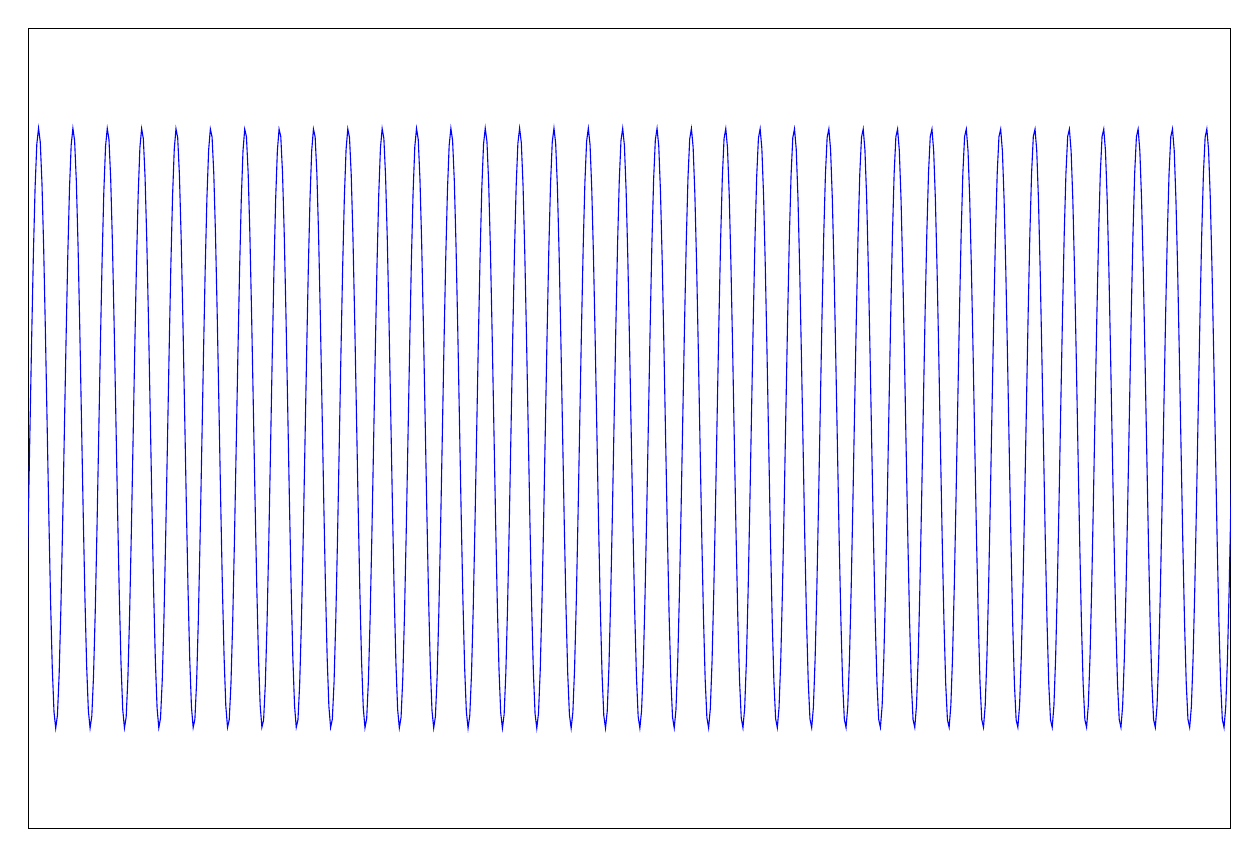
\begin{tikzpicture}

\begin{axis}[%
width=6.01339838214984in,
height=4in,
scale only axis,
xmin=100,
xmax=800,
ymin=-0.4,
ymax=0.4,
ticks=none,
xticklabels={\empty}
]
\addplot [color=blue,solid,forget plot]
  table[row sep=crcr]{1	0.0112375593608282\\
2	0.104054027270611\\
3	0.185659443540537\\
4	0.249116295067321\\
5	0.288637090749755\\
6	0.299777867539804\\
7	0.281623510020854\\
8	0.23610628156478\\
9	0.167790360278693\\
10	0.0825485590193881\\
11	-0.0106015014344606\\
12	-0.102529122373024\\
13	-0.184317183180363\\
14	-0.248615534911024\\
15	-0.288360673246228\\
16	-0.299821281220836\\
17	-0.282068826668459\\
18	-0.237009712391777\\
19	-0.168423918253911\\
20	-0.0834793879375805\\
21	0.00941865463469753\\
22	0.101194926602266\\
23	0.183689294117423\\
24	0.248001128365307\\
25	0.287973002957407\\
26	0.299877541741918\\
27	0.282456755518574\\
28	0.237912798895348\\
29	0.169242660776412\\
30	0.0848192539847733\\
31	-0.00761837071740019\\
32	-0.0999323184800757\\
33	-0.182280679495485\\
34	-0.247221538531601\\
35	-0.287442031987116\\
36	-0.299916175524785\\
37	-0.283145319878605\\
38	-0.238448684998989\\
39	-0.170437165997998\\
40	-0.085936874433079\\
41	0.0067079922343034\\
42	0.0992666885438733\\
43	0.18119893350842\\
44	0.246539200766412\\
45	0.287146224000055\\
46	0.29993762093401\\
47	0.283401704589276\\
48	0.239378255199546\\
49	0.171659781408742\\
50	0.0873324227062733\\
51	-0.00526529471435114\\
52	-0.0978836738063544\\
53	-0.180019052367934\\
54	-0.245651672299934\\
55	-0.286672392084536\\
56	-0.299968076301883\\
57	-0.284009985716896\\
58	-0.240107237249115\\
59	-0.172808940516944\\
60	-0.0888720343293032\\
61	0.00343116031233622\\
62	0.0958974780711973\\
63	0.179403776639671\\
64	0.244561734192625\\
65	0.286250318176386\\
66	0.29999171429595\\
67	0.284457597782985\\
68	0.241193360502576\\
69	0.174015302764896\\
70	0.090718850371994\\
71	-0.00257143363262935\\
72	-0.0945898492355176\\
73	-0.177845451330406\\
74	-0.243558650299533\\
75	-0.285780826363441\\
76	-0.300002922123118\\
77	-0.284877626883362\\
78	-0.241937929523447\\
79	-0.175628285826437\\
80	-0.0918632453240638\\
81	0.000578380379041642\\
82	0.0933729747871525\\
83	0.176743498018826\\
84	0.242696516245057\\
85	0.285283043298781\\
86	0.300006165464375\\
87	0.285504183839068\\
88	0.242836772911666\\
89	0.177075130776372\\
90	0.093167561758634\\
91	0.00112606033680896\\
92	-0.0913898262061582\\
93	-0.175313601237434\\
94	-0.241827844845546\\
95	-0.284899880015489\\
96	-0.300003226603007\\
97	-0.285982425856583\\
98	-0.244099299146542\\
99	-0.178155689420278\\
100	-0.0950727309735491\\
101	-0.0023969850562007\\
102	0.0901611189229004\\
103	0.173643138568475\\
104	0.240963238524448\\
105	0.284174443874572\\
106	0.299988172006713\\
107	0.286366040863395\\
108	0.244982447039306\\
109	0.179617830420892\\
110	0.0964645378184282\\
111	0.00423890328953314\\
112	-0.0880238872318821\\
113	-0.172557491339168\\
114	-0.239861820317097\\
115	-0.283628396746788\\
116	-0.299954340259848\\
117	-0.287021180258964\\
118	-0.245875761113755\\
119	-0.18089044867354\\
120	-0.098669326539597\\
121	-0.00604937777521506\\
122	0.0867563550333993\\
123	0.170757443319199\\
124	0.23876945543491\\
125	0.283149866080037\\
126	0.299917324434594\\
127	0.287479793568311\\
128	0.247038648664814\\
129	0.182415089719173\\
130	0.100378026872305\\
131	0.00784046751674588\\
132	-0.0850328335501926\\
133	-0.169239215933411\\
134	-0.237573622786092\\
135	-0.282442068289872\\
136	-0.299870356349823\\
137	-0.288037619220752\\
138	-0.247995350320755\\
139	-0.184033701989515\\
140	-0.102111167696166\\
141	-0.010151647823681\\
142	0.0828946745558184\\
143	0.167922617483927\\
144	0.236217422431687\\
145	0.281854265397597\\
146	0.299808549150762\\
147	0.288599447797963\\
148	0.249258433965014\\
149	0.185578173034263\\
150	0.103740544775203\\
151	0.0117186282080908\\
152	-0.0809639602580095\\
153	-0.166296975050464\\
154	-0.235017018844395\\
155	-0.281170696736489\\
156	-0.299725483614238\\
157	-0.28905349379556\\
158	-0.250318905161816\\
159	-0.186872783442049\\
160	-0.10557519335059\\
161	-0.0140473668796044\\
162	0.0793356931855125\\
163	0.164495667635178\\
164	0.234000558700958\\
165	0.28057317583298\\
166	0.29964122661185\\
167	0.28957337152427\\
168	0.251229670635474\\
169	0.188370463930901\\
170	0.107192757099051\\
171	0.0156179967340141\\
172	-0.0774191336259189\\
173	-0.163277887818999\\
174	-0.232778165104032\\
175	-0.279845796427311\\
176	-0.299556884402294\\
177	-0.290029307056149\\
178	-0.252294320194841\\
179	-0.190067078497345\\
180	-0.109046733766561\\
181	-0.0174305217523798\\
182	0.0757763910656362\\
183	0.161525157551632\\
184	0.231782315553456\\
185	0.279113145736286\\
186	0.299436643852756\\
187	0.290445421510679\\
188	0.253225045546788\\
189	0.191134599270342\\
190	0.110461866990029\\
191	0.0191199523740884\\
192	-0.0739898754670617\\
193	-0.160169381268816\\
194	-0.230620055168004\\
195	-0.278533921543273\\
196	-0.299345126003325\\
197	-0.290953876435106\\
198	-0.254200440032958\\
199	-0.192394622908404\\
200	-0.112176209685748\\
201	-0.0207544679636095\\
202	0.0726149305247711\\
203	0.158828337358542\\
204	0.229771606558825\\
205	0.277984430335479\\
206	0.299234520266135\\
207	0.291249860627523\\
208	0.254858719199907\\
209	0.193654696755593\\
210	0.113266659941355\\
211	0.0222045747734398\\
212	-0.0713618016682545\\
213	-0.157919013364711\\
214	-0.229010219503948\\
215	-0.277539539146801\\
216	-0.299155528022457\\
217	-0.291481950512762\\
218	-0.255449806760833\\
219	-0.194266041440522\\
220	-0.114334821236447\\
221	-0.0228250037073524\\
222	0.0706362038757387\\
223	0.156954685923511\\
224	0.228346235018431\\
225	0.277239190311472\\
226	0.299090038913477\\
227	0.291634481437101\\
228	0.255651657982665\\
229	0.194816023042601\\
230	0.114820274910397\\
231	0.0233755342407119\\
232	-0.0698770592422766\\
233	-0.156554365757119\\
234	-0.228106483042188\\
235	-0.277062957489631\\
236	-0.29906151807601\\
237	-0.291754071290981\\
238	-0.255883212323356\\
239	-0.194964487534305\\
240	-0.114945860125818\\
241	-0.0236366751253523\\
242	0.0700409155182462\\
243	0.156594101452823\\
244	0.228179155898745\\
245	0.277202435616442\\
246	0.299067032952988\\
247	0.291680326637097\\
248	0.255680528470692\\
249	0.194758567973111\\
250	0.114635408690245\\
251	0.0234287306989521\\
252	-0.070293652498048\\
253	-0.1570052486884\\
254	-0.228510263721418\\
255	-0.277327339905378\\
256	-0.299121723695321\\
257	-0.291579661997024\\
258	-0.255496061928648\\
259	-0.194148806582269\\
260	-0.114048939982222\\
261	-0.022442882407689\\
262	0.0709853627895671\\
263	0.157813755227611\\
264	0.228865877098285\\
265	0.277722772445114\\
266	0.299188467499925\\
267	0.291290811187834\\
268	0.254828125435915\\
269	0.193360097950802\\
270	0.112877365825646\\
271	0.0212386027585478\\
272	-0.0721782251947352\\
273	-0.158961907871913\\
274	-0.229846799874633\\
275	-0.278227847458412\\
276	-0.299276116674018\\
277	-0.291003977581619\\
278	-0.2541969144287\\
279	-0.192411021441981\\
280	-0.111646228311201\\
281	-0.0197687992901933\\
282	0.0737557718620985\\
283	0.160132173193288\\
284	0.230867121428946\\
285	0.278756810496545\\
286	0.299381690496978\\
287	0.290645171979842\\
288	0.253276070379396\\
289	0.191214257601351\\
290	0.109935919546954\\
291	0.0180929078543032\\
292	-0.0751761623485204\\
293	-0.161599877921191\\
294	-0.231840197421598\\
295	-0.279391165933639\\
296	-0.299506739205565\\
297	-0.290226379861303\\
298	-0.252292808002177\\
299	-0.189704567885351\\
300	-0.108437806554459\\
301	-0.0164173018560925\\
302	0.0772906910891075\\
303	0.163046626240184\\
304	0.232898726934937\\
305	0.28014774707427\\
306	0.29961582017589\\
307	0.289762563638388\\
308	0.251418224653192\\
309	0.188262320188605\\
310	0.106512940457331\\
311	0.0147103290989609\\
312	-0.0790629363182466\\
313	-0.164610940252596\\
314	-0.234077192267248\\
315	-0.280805046243487\\
316	-0.29969566477326\\
317	-0.289218767804095\\
318	-0.250376924627627\\
319	-0.186569672928664\\
320	-0.104771074009466\\
321	-0.0127037183260243\\
322	0.080592160385127\\
323	0.16642208563072\\
324	0.235412927125954\\
325	0.281352082976987\\
326	0.299783132711688\\
327	0.288730308377377\\
328	0.24921058060302\\
329	0.185132323451613\\
330	0.102853813533004\\
331	0.0110895507565488\\
332	-0.0827784052278759\\
333	-0.16788191217496\\
334	-0.23648250943687\\
335	-0.282115431926672\\
336	-0.299839132751279\\
337	-0.288209462504306\\
338	-0.24828323090244\\
339	-0.183594829864307\\
340	-0.10136646478014\\
341	-0.00876344161358123\\
342	0.084577927358015\\
343	0.169482444415843\\
344	0.237666292236689\\
345	0.282752356235294\\
346	0.299901427095065\\
347	0.28758501923239\\
348	0.247145076802499\\
349	0.182186952021795\\
350	0.0994192265821275\\
351	0.00706627865585365\\
352	-0.086396195860564\\
353	-0.171161986874845\\
354	-0.23895826277815\\
355	-0.283265964163941\\
356	-0.299944960939511\\
357	-0.287160429145008\\
358	-0.245998086260375\\
359	-0.180711839881067\\
360	-0.0978729110070249\\
361	-0.00504059128725217\\
362	0.088051883091927\\
363	0.172285901407436\\
364	0.239931584915451\\
365	0.283853801859493\\
366	0.299974773417793\\
367	0.286546612174885\\
368	0.245150489800154\\
369	0.179511653386059\\
370	0.0958359864276279\\
371	0.00363499826417101\\
372	-0.0899392018156172\\
373	-0.173759176455929\\
374	-0.240890292491698\\
375	-0.284509621863798\\
376	-0.299997359515192\\
377	-0.286128293401565\\
378	-0.244149783004769\\
379	-0.177890576816005\\
380	-0.0943499444265777\\
381	-0.0018919970699802\\
382	0.0910868868936795\\
383	0.17540015097609\\
384	0.242129227769262\\
385	0.284951656798339\\
386	0.299999527361273\\
387	0.285487285889869\\
388	0.24297118987422\\
389	0.176348883242863\\
390	0.0926855428108161\\
391	0.000349459703539682\\
392	-0.0930390778004778\\
393	-0.176852868251936\\
394	-0.243004123946602\\
395	-0.285533636339276\\
396	-0.300001995571618\\
397	-0.28491768174853\\
398	-0.242159505031441\\
399	-0.175006388192929\\
400	-0.0916176353337047\\
401	0.001718019791129\\
402	0.09444978333789\\
403	0.178159736093328\\
404	0.244002753532735\\
405	0.286074190248099\\
406	0.299995583451329\\
407	0.284595081945042\\
408	0.241117730740943\\
409	0.174254057575489\\
410	0.0900996558134009\\
411	-0.00319627928446005\\
412	-0.0957002225355136\\
413	-0.179073683578422\\
414	-0.244992397402258\\
415	-0.286509915899487\\
416	-0.299972215358782\\
417	-0.284059720536585\\
418	-0.240316191406775\\
419	-0.17280916927769\\
420	-0.0880173408535955\\
421	0.00495313803586388\\
422	0.0976917871472481\\
423	0.180367108012491\\
424	0.245629836332489\\
425	0.286915502042277\\
426	0.299958623716707\\
427	0.283460423398204\\
428	0.239089266009175\\
429	0.171676136515527\\
430	0.0873437434853588\\
431	-0.00577048133828395\\
432	-0.0985560520084902\\
433	-0.181144124058912\\
434	-0.24669176071819\\
435	-0.2872180793289\\
436	-0.299921391317911\\
437	-0.28312929402411\\
438	-0.238517483217089\\
439	-0.170278316425704\\
440	-0.085817422601102\\
441	0.00724583855131347\\
442	0.0998231827824174\\
443	0.182754771864631\\
444	0.247246949120847\\
445	0.287672607946677\\
446	0.299886295551042\\
447	0.282771221360836\\
448	0.237500062040361\\
449	0.169138540123689\\
450	0.0839748001360038\\
451	-0.00879983240552822\\
452	-0.10091852041746\\
453	-0.183356552411278\\
454	-0.247935116572917\\
455	-0.288143256109577\\
456	-0.299849250387457\\
457	-0.282227282036941\\
458	-0.236824544727081\\
459	-0.167940781975734\\
460	-0.0831100696789355\\
461	0.0100274705679842\\
462	0.102363123205186\\
463	0.184791580801326\\
464	0.248594399487864\\
465	0.288287297347702\\
466	0.299793465129982\\
467	0.281898298442507\\
468	0.236105972689515\\
469	0.167582579823939\\
470	0.0816806205400565\\
471	-0.0116467651633384\\
472	-0.103145241427887\\
473	-0.185533314260566\\
474	-0.249161668769187\\
475	-0.288833710297502\\
476	-0.299748943706754\\
477	-0.281497078873918\\
478	-0.235370001094641\\
479	-0.166602028688525\\
480	-0.0805472483429496\\
481	0.0127906999714842\\
482	0.104154916527722\\
483	0.186327207060333\\
484	0.25019330150406\\
485	0.289059640372384\\
486	0.299716875067351\\
487	0.280968393571809\\
488	0.234520390523751\\
489	0.165606962195794\\
490	0.0795478740968438\\
491	-0.0136262771206323\\
492	-0.105605763595907\\
493	-0.187363148332173\\
494	-0.250798786456623\\
495	-0.289282303883937\\
496	-0.299688486130094\\
497	-0.280541527376535\\
498	-0.233953003072044\\
499	-0.164303385542386\\
500	-0.0792925473949801\\
501	0.014481055461008\\
502	0.1060620708672\\
503	0.188218612643761\\
504	0.251182257435885\\
505	0.289603712201916\\
506	0.299604625090123\\
507	0.280409124409813\\
508	0.233374584435724\\
509	0.163939245095048\\
510	0.0784196707686497\\
511	-0.0158895772012837\\
512	-0.10690897210468\\
513	-0.188505327484439\\
514	-0.251620515981318\\
515	-0.289678544998301\\
516	-0.29956673543073\\
517	-0.28001491259578\\
518	-0.233072588357347\\
519	-0.163209419699253\\
520	-0.0772049088020185\\
521	0.0165074521546294\\
522	0.107785521848022\\
523	0.189514741972315\\
524	0.251963567828808\\
525	0.289909987632952\\
526	0.299501196452363\\
527	0.279831392269158\\
528	0.232564601931876\\
529	0.162325252141693\\
530	0.0759495028022723\\
531	-0.0170632626714264\\
532	-0.109453140291079\\
533	-0.190275487862462\\
534	-0.252615854549268\\
535	-0.290268713710216\\
536	-0.299462354684511\\
537	-0.279197240050848\\
538	-0.231995244252587\\
539	-0.161423646484309\\
540	-0.0757692225675667\\
541	0.018381893805406\\
542	0.109864986355638\\
543	0.190697399803762\\
544	0.252950444227011\\
545	0.290454607526773\\
546	0.299413390627371\\
547	0.279251225566979\\
548	0.231419583120898\\
549	0.160607624884067\\
550	0.0747993374408725\\
551	-0.018371759446418\\
552	-0.110827279873276\\
553	-0.191502361695329\\
554	-0.253502504827331\\
555	-0.290704320023654\\
556	-0.299418141912627\\
557	-0.278902569934836\\
558	-0.230845234363222\\
559	-0.160776263128662\\
560	-0.0740469792088834\\
561	0.0190632908429572\\
562	0.111390838466733\\
563	0.191897263944719\\
564	0.253718172426735\\
565	0.290772374537796\\
566	0.299342983293564\\
567	0.278508439034495\\
568	0.230255826672454\\
569	0.160138698289169\\
570	0.0734689887747117\\
571	-0.0194788329063458\\
572	-0.111609590977259\\
573	-0.191926973133258\\
574	-0.254191222703894\\
575	-0.290937432630517\\
576	-0.299312504791759\\
577	-0.278426723401722\\
578	-0.230269361290979\\
579	-0.159476301937658\\
580	-0.0729616097190101\\
581	0.0207870316373497\\
582	0.111588755149932\\
583	0.192498839538825\\
584	0.254431951672948\\
585	0.290975198752278\\
586	0.299249052971804\\
587	0.278214356626125\\
588	0.230117822375678\\
589	0.15865579253317\\
590	0.0723678723630357\\
591	-0.0210417996944514\\
592	-0.11247466241367\\
593	-0.192938725028206\\
594	-0.254534667392527\\
595	-0.291188427357916\\
596	-0.299213719082084\\
597	-0.277792436456556\\
598	-0.229665730521853\\
599	-0.158416513903486\\
600	-0.0725271282046802\\
601	0.0215123152822032\\
602	0.112486727322435\\
603	0.193415291861333\\
604	0.254620179020601\\
605	0.291364893019579\\
606	0.299193739125311\\
607	0.277882067839143\\
608	0.229438682740516\\
609	0.158563980334015\\
610	0.0721557480362903\\
611	-0.0224582851939305\\
612	-0.112852725255997\\
613	-0.193303209289885\\
614	-0.254827983696118\\
615	-0.291318702973943\\
616	-0.299170991694224\\
617	-0.277566261584958\\
618	-0.229273643299477\\
619	-0.157937581920363\\
620	-0.0709603695953195\\
621	0.0219912547853012\\
622	0.113852193739862\\
623	0.193660034417458\\
624	0.255303997724683\\
625	0.291381500790285\\
626	0.299123576932881\\
627	0.277538560727217\\
628	0.228972393823046\\
629	0.157181154863052\\
630	0.0707495609795946\\
631	-0.0225930378152698\\
632	-0.113773679505498\\
633	-0.193888380554395\\
634	-0.255081991400932\\
635	-0.291376198517632\\
636	-0.299093377559499\\
637	-0.277279140892979\\
638	-0.228308509852851\\
639	-0.157864960507638\\
640	-0.0712192177050529\\
641	0.0224414443895584\\
642	0.113939200189669\\
643	0.194253332721968\\
644	0.255500764847822\\
645	0.291635068381731\\
646	0.299151873404447\\
647	0.277482855660387\\
648	0.228459465802232\\
649	0.156908165934899\\
650	0.0709410250855776\\
651	-0.0229978112888876\\
652	-0.114673572957094\\
653	-0.194208901068754\\
654	-0.255599907298989\\
655	-0.291466908193198\\
656	-0.299108063444763\\
657	-0.277158296469089\\
658	-0.228490090051739\\
659	-0.156784170866881\\
660	-0.0705979806861048\\
661	0.0235242683864564\\
662	0.11430885805717\\
663	0.194888944741467\\
664	0.255565898636421\\
665	0.291493344276065\\
666	0.299089592918642\\
667	0.277422979233661\\
668	0.228147719659932\\
669	0.157149516514025\\
670	0.0698314556116394\\
671	-0.0233225582830936\\
672	-0.114235744158759\\
673	-0.194894028607158\\
674	-0.255622440345891\\
675	-0.291543790077769\\
676	-0.299062719385684\\
677	-0.277293957982834\\
678	-0.228588372793079\\
679	-0.156740966107719\\
680	-0.0703940686036791\\
681	0.0228065000465975\\
682	0.114801448876213\\
683	0.194545424295134\\
684	0.255403611174818\\
685	0.291700314333262\\
686	0.299097364572183\\
687	0.277444012234854\\
688	0.228128824134376\\
689	0.157096136584384\\
690	0.0708001742464438\\
691	-0.0234561805061995\\
692	-0.114353387279838\\
693	-0.194999393632413\\
694	-0.255681326626401\\
695	-0.291557868289535\\
696	-0.299065814946152\\
697	-0.277300683983013\\
698	-0.228660534478835\\
699	-0.156908585988796\\
700	-0.0706779184572233\\
701	0.0234834107259865\\
702	0.114300125503\\
703	0.194860565872571\\
704	0.255529122137698\\
705	0.291724882028024\\
706	0.299102335250502\\
707	0.277142025892032\\
708	0.228472523054891\\
709	0.156792443730543\\
710	0.0707045069015897\\
711	-0.0233069636372536\\
712	-0.113967656265852\\
713	-0.194451414525277\\
714	-0.255737029303082\\
715	-0.291505280722783\\
716	-0.299105638029589\\
717	-0.277224922814672\\
718	-0.228744804542867\\
719	-0.157349803038392\\
720	-0.0704777998747652\\
721	0.0232970055867207\\
722	0.113733289851002\\
723	0.194081630307555\\
724	0.255336884096652\\
725	0.291525104584727\\
726	0.29912516527812\\
727	0.277396160273101\\
728	0.228523031637741\\
729	0.157297761150969\\
730	0.0707089919978454\\
731	-0.0227464378634943\\
732	-0.113963043857109\\
733	-0.194016853145302\\
734	-0.255119936092144\\
735	-0.291358585190949\\
736	-0.299117334338863\\
737	-0.277527447055101\\
738	-0.228975379520608\\
739	-0.157260931196617\\
740	-0.0710396242161504\\
741	0.0220411890022942\\
742	0.113960213235312\\
743	0.193710415307192\\
744	0.255281643131748\\
745	0.291326323007766\\
746	0.29915653598605\\
747	0.277478564061208\\
748	0.229149916984176\\
749	0.157880070975918\\
750	0.0711173026106135\\
751	-0.0215240795111276\\
752	-0.113042814193589\\
753	-0.193433969760987\\
754	-0.254842847633784\\
755	-0.291268098334223\\
756	-0.299212634662179\\
757	-0.277935061904526\\
758	-0.22955732252877\\
759	-0.157937539728734\\
760	-0.0716740340559388\\
761	0.0215017076047528\\
762	0.11252700173335\\
763	0.193430793110517\\
764	0.254542755459389\\
765	0.291258338025936\\
766	0.299261046960719\\
767	0.277966578768061\\
768	0.229300440701196\\
769	0.159008567269061\\
770	0.0724247988555108\\
771	-0.0211952611921554\\
772	-0.112679715626755\\
773	-0.193082277696143\\
774	-0.254536931705743\\
775	-0.291106367587294\\
776	-0.299272247787675\\
777	-0.278286822031726\\
778	-0.229589735813891\\
779	-0.159034354263188\\
780	-0.07311059219427\\
781	0.0208729886596031\\
782	0.11175119375062\\
783	0.192593761434479\\
784	0.254389882441704\\
785	0.290870142767576\\
786	0.299313672003517\\
787	0.278400331314863\\
788	0.230260209684801\\
789	0.159641921604359\\
790	0.0735092972364674\\
791	-0.0197031675001395\\
792	-0.111919442274286\\
793	-0.19213384167411\\
794	-0.253654109555733\\
795	-0.290856641644429\\
796	-0.299300468024893\\
797	-0.278629855032147\\
798	-0.230505117240401\\
799	-0.159773135993662\\
800	-0.0734492212496514\\
801	0.0199728967433427\\
802	0.111376582321705\\
803	0.191832869532848\\
804	0.253542532697222\\
805	0.290587578572506\\
806	0.299363254091551\\
807	0.278915199367895\\
808	0.230910116929367\\
809	0.160202288583338\\
810	0.0748241164208721\\
811	-0.0186692415491117\\
812	-0.110254098576973\\
813	-0.190981354993184\\
814	-0.252996358524542\\
815	-0.290606241380054\\
816	-0.299422450566215\\
817	-0.279218725112737\\
818	-0.231410696761861\\
819	-0.160848646796354\\
820	-0.0755256365082095\\
821	0.0179612186930153\\
822	0.109588053864795\\
823	0.19042801994844\\
824	0.252606566443877\\
825	0.290413180506125\\
826	0.299471050821075\\
827	0.279157674966775\\
828	0.231982379653393\\
829	0.161674845575027\\
830	0.0755677947151697\\
831	-0.0178409711075983\\
832	-0.109378701198924\\
833	-0.190155431823835\\
834	-0.252362650150811\\
835	-0.290265356030773\\
836	-0.299509228195206\\
837	-0.279491704352273\\
838	-0.23265056893045\\
839	-0.162705331789718\\
840	-0.0769491321281617\\
841	0.0162149854255096\\
842	0.108616888142263\\
843	0.189349070955668\\
844	0.252203286083181\\
845	0.289882719637162\\
846	0.299553748445901\\
847	0.279863292115417\\
848	0.23286013499555\\
849	0.163218779846856\\
850	0.0778125736009029\\
851	-0.0159849622553138\\
852	-0.107159677073038\\
853	-0.18866417557766\\
854	-0.251535879494589\\
855	-0.289717696748096\\
856	-0.299607560781636\\
857	-0.280355863241097\\
858	-0.233341941773194\\
859	-0.164211351934794\\
860	-0.0784271875335105\\
861	0.0149329691955583\\
862	0.106686306912831\\
863	0.187894362726024\\
864	0.250737392997057\\
865	0.289474779222492\\
866	0.299631494949109\\
867	0.280700507171816\\
868	0.234294834949082\\
869	0.16510602350044\\
870	0.0790429116425228\\
871	-0.0137262448074969\\
872	-0.105906790527856\\
873	-0.187545821252307\\
874	-0.250179646587591\\
875	-0.289289388982138\\
876	-0.299692157502738\\
877	-0.281054640510169\\
878	-0.234726775456366\\
879	-0.165435855284521\\
880	-0.080098834929157\\
881	0.012887901637032\\
882	0.104469741970478\\
883	0.186529231947036\\
884	0.249576749900452\\
885	0.288793507692927\\
886	0.299764161170021\\
887	0.281251093008118\\
888	0.235558417005078\\
889	0.166452821558765\\
890	0.0811683740742273\\
891	-0.0118825297463947\\
892	-0.103614134203509\\
893	-0.185136644604335\\
894	-0.249133494743609\\
895	-0.288585806197319\\
896	-0.299793661277893\\
897	-0.281828638315175\\
898	-0.236035017309848\\
899	-0.167878168273363\\
900	-0.0828672463982933\\
901	0.0100525710687425\\
902	0.102663730804934\\
903	0.184266011609485\\
904	0.248450999640169\\
905	0.28821317308805\\
906	0.299845624620133\\
907	0.282098493063515\\
908	0.236649671494359\\
909	0.168857667383755\\
910	0.0833611534743443\\
911	-0.00930063496556918\\
912	-0.101692041966885\\
913	-0.183226576225454\\
914	-0.24803760155548\\
915	-0.287926088209844\\
916	-0.299863627294157\\
917	-0.282679824274386\\
918	-0.237938169415242\\
919	-0.169481028398677\\
920	-0.0853260036633578\\
921	0.00771386713398231\\
922	0.0997822905133552\\
923	0.182629512288473\\
924	0.246835111341387\\
925	0.287419373917264\\
926	0.299904228232987\\
927	0.283058956566168\\
928	0.238445938977626\\
929	0.170654008417075\\
930	0.086447738703159\\
931	-0.00674659712807175\\
932	-0.0990454772999646\\
933	-0.181466446903535\\
934	-0.246098027298823\\
935	-0.287085786463278\\
936	-0.29994647378457\\
937	-0.283381482153053\\
938	-0.239509047979521\\
939	-0.172072249000776\\
940	-0.0873010242664558\\
941	0.005010649138775\\
942	0.0973698851018032\\
943	0.180008604627266\\
944	0.245475774219098\\
945	0.286734351987264\\
946	0.299969923744373\\
947	0.283875320432676\\
948	0.240038149149889\\
949	0.172964511780408\\
950	0.0893462802085846\\
951	-0.0034253231557954\\
952	-0.0963503396007635\\
953	-0.178898769433727\\
954	-0.244474819033751\\
955	-0.286346448869155\\
956	-0.299991471371958\\
957	-0.284557719449458\\
958	-0.241108831244469\\
959	-0.174166139566628\\
960	-0.0904692989427364\\
961	0.0024997241206012\\
962	0.0949378440618198\\
963	0.177869569171417\\
964	0.243825751256605\\
965	0.285816020096077\\
966	0.300000377957454\\
967	0.284819686801589\\
968	0.242034400250451\\
969	0.175432480867536\\
970	0.091969891133015\\
971	-0.0008604194126244\\
972	-0.093299818560891\\
973	-0.176390968923577\\
974	-0.242664081311601\\
975	-0.285381218594106\\
976	-0.300005703681695\\
977	-0.285408279705092\\
978	-0.242874128008569\\
979	-0.176840407947425\\
980	-0.0932534350672161\\
981	-0.000872849135017431\\
982	0.0912657143645827\\
983	0.175475512324946\\
984	0.241715748307705\\
985	0.284717267268988\\
986	0.300001654095295\\
987	0.285968134349328\\
988	0.243895484216698\\
989	0.178199923299957\\
990	0.0948478525955361\\
991	0.00257079579762506\\
992	-0.0896036288860426\\
993	-0.173958310571883\\
994	-0.240944008197083\\
995	-0.284250222500529\\
996	-0.299986902525991\\
997	-0.286549946379258\\
998	-0.245193881177875\\
999	-0.179716830814401\\
1000	-0.0969936061777435\\
1001	-0.00456622201856015\\
1002	0.0879267071487003\\
1003	0.172107301326391\\
1004	0.239662644279997\\
1005	0.283591513843026\\
1006	0.299957602542117\\
1007	0.286942560836311\\
1008	0.245984591803235\\
1009	0.181409342586659\\
1010	0.0985081358526003\\
1011	0.00635167517169444\\
1012	-0.0866261251776665\\
1013	-0.170778461218256\\
1014	-0.238493862415205\\
1015	-0.283047519308088\\
1016	-0.299910319416602\\
1017	-0.287484495453051\\
1018	-0.246992433508019\\
1019	-0.182735366541733\\
1020	-0.100068331207393\\
1021	-0.00801658819204922\\
1022	0.0843796874418677\\
1023	0.169264233930878\\
1024	0.237277342332625\\
1025	0.282507584126483\\
1026	0.299854958703014\\
1027	0.288108447388326\\
1028	0.248103000757594\\
1029	0.184132360567974\\
1030	0.102175261464785\\
1031	0.0101738698056829\\
1032	-0.0829090814567563\\
1033	-0.167959640251835\\
1034	-0.236259103429544\\
1035	-0.281700533577478\\
1036	-0.299813272443139\\
1037	-0.288561268900265\\
1038	-0.24919192719861\\
1039	-0.18549118565109\\
1040	-0.103642014213135\\
1041	-0.0121757271131489\\
1042	0.0810263699233356\\
1043	0.166323900992117\\
1044	0.235025466483082\\
1045	0.281158085760698\\
1046	0.299712890634799\\
1047	0.289095257732745\\
1048	0.250424540899245\\
1049	0.187063366730984\\
1050	0.105877822414921\\
1051	0.0139168039468138\\
1052	-0.0793882591565103\\
1053	-0.164459650249443\\
1054	-0.23392655025572\\
1055	-0.280492918883907\\
1056	-0.299647259762136\\
1057	-0.28969052626073\\
1058	-0.251240957814882\\
1059	-0.188494048538234\\
1060	-0.107439174397893\\
1061	-0.0160091055961165\\
1062	0.0773895511515961\\
1063	0.16314368303206\\
1064	0.232586101516959\\
1065	0.279693824876842\\
1066	0.29954767369068\\
1067	0.290100348577452\\
1068	0.252252669467933\\
1069	0.190142056703407\\
1070	0.109268290145526\\
1071	0.0178394938343814\\
1072	-0.0756754717086594\\
1073	-0.161300873425569\\
1074	-0.231498814863128\\
1075	-0.279062072767323\\
1076	-0.299438920064414\\
1077	-0.290575828604229\\
1078	-0.253337406983422\\
1079	-0.191434037943176\\
1080	-0.110581259249898\\
1081	-0.0194061330866803\\
1082	0.0739571785975364\\
1083	0.159994785095812\\
1084	0.230660169901069\\
1085	0.278491877764511\\
1086	0.299323178589292\\
1087	0.290961144594767\\
1088	0.254071373417813\\
1089	0.192651559637281\\
1090	0.112251206430211\\
1091	0.0209816541026357\\
1092	-0.072657299358199\\
1093	-0.158747175541413\\
1094	-0.229620187048076\\
1095	-0.277997599356241\\
1096	-0.299230191587091\\
1097	-0.291295599610141\\
1098	-0.254803395339484\\
1099	-0.193648911441715\\
1100	-0.113343578083424\\
1101	-0.0219749224692323\\
1102	0.0715168475313588\\
1103	0.157674534844187\\
1104	0.228794841537062\\
1105	0.277546811669699\\
1106	0.299155079677633\\
1107	0.291485371291265\\
1108	0.255455285092072\\
1109	0.194261187067957\\
1110	0.114298463403942\\
1111	0.0231155605898375\\
1112	-0.0704156929325113\\
1113	-0.157150992167543\\
1114	-0.228314985202902\\
1115	-0.277265059040169\\
1116	-0.29910618091681\\
1117	-0.291641685000971\\
1118	-0.255774021248262\\
1119	-0.19485276384945\\
1120	-0.114676847613045\\
1121	-0.0233679288883251\\
1122	0.0701205644415021\\
1123	0.156676777005951\\
1124	0.228143493311191\\
1125	0.277200299921363\\
1126	0.299055912710319\\
1127	0.291769341842137\\
1128	0.255920755866398\\
1129	0.195005824783296\\
1130	0.11496006230261\\
1131	0.023592100839505\\
1132	-0.0701631470866814\\
1133	-0.156787498564051\\
1134	-0.228165399334412\\
1135	-0.277248117890898\\
1136	-0.299087946279188\\
1137	-0.291656321354326\\
1138	-0.255717972235223\\
1139	-0.194645904548449\\
1140	-0.114622688317609\\
1141	-0.0231576753954516\\
1142	0.0704623518962599\\
1143	0.157083270176514\\
1144	0.228527673301737\\
1145	0.277462856516927\\
1146	0.299146382197741\\
1147	0.291507924219786\\
1148	0.255338492518698\\
1149	0.19420475119593\\
1150	0.113739713796888\\
1151	0.0224604669115922\\
1152	-0.0713909625453895\\
1153	-0.157886692536154\\
1154	-0.228965756199112\\
1155	-0.277812067043738\\
1156	-0.299212410597533\\
1157	-0.291284014361159\\
1158	-0.25475759680668\\
1159	-0.193172016360847\\
1160	-0.112912493144082\\
1161	-0.0211419947513503\\
1162	0.0724061343561896\\
1163	0.158933772293919\\
1164	0.229914745403917\\
1165	0.278327830201858\\
1166	0.299306677746524\\
1167	0.290962312080429\\
1168	0.2540201818909\\
1169	0.192035944758609\\
1170	0.111417683119193\\
1171	0.0197735985699318\\
1172	-0.0739075247872378\\
1173	-0.160417820632736\\
1174	-0.230923038729244\\
1175	-0.278847841894275\\
1176	-0.299413891945045\\
1177	-0.290602108983312\\
1178	-0.253086271368823\\
1179	-0.190819267209879\\
1180	-0.109694808650298\\
1181	-0.0181294395213192\\
1182	0.075313016802054\\
1183	0.161865708999631\\
1184	0.2318453206802\\
1185	0.279460494696906\\
1186	0.299520497504895\\
1187	0.290101598274991\\
1188	0.252184551591411\\
1189	0.189446473903874\\
1190	0.10841939957828\\
1191	0.0162661741867349\\
1192	-0.0771184499794885\\
1193	-0.163410736297703\\
1194	-0.233263534678363\\
1195	-0.280224053993668\\
1196	-0.299604952681241\\
1197	-0.289649975575196\\
1198	-0.251097624245704\\
1199	-0.188128899727032\\
1200	-0.106718432727429\\
1201	-0.0143231707391143\\
1202	0.0790252889131076\\
1203	0.164663071971993\\
1204	0.234158386385397\\
1205	0.280880094442741\\
1206	0.299714218532782\\
1207	0.289117990770417\\
1208	0.25014756768685\\
1209	0.186622529112671\\
1210	0.104779283330548\\
1211	0.0126757836886209\\
1212	-0.0806481152713719\\
1213	-0.166503371413707\\
1214	-0.235491347903973\\
1215	-0.28139641997388\\
1216	-0.299785640512815\\
1217	-0.288694217845345\\
1218	-0.249123864513538\\
1219	-0.185007135171822\\
1220	-0.102723824733954\\
1221	-0.010400346727548\\
1222	0.0828682735627634\\
1223	0.167937707079373\\
1224	0.236858096874344\\
1225	0.282107648498011\\
1226	0.29984786908024\\
1227	0.288085526738536\\
1228	0.248060713562572\\
1229	0.183803000149706\\
1230	0.101121805154201\\
1231	0.00858520187932153\\
1232	-0.0846649723355832\\
1233	-0.169477674173321\\
1234	-0.237971261127875\\
1235	-0.282672040871995\\
1236	-0.299899385845006\\
1237	-0.287539738021457\\
1238	-0.247122474482317\\
1239	-0.182259535548135\\
1240	-0.0996379352339583\\
1241	-0.00681480175888847\\
1242	0.0864960146770928\\
1243	0.171118527666816\\
1244	0.238826025478202\\
1245	0.283348266435852\\
1246	0.299943900386213\\
1247	0.286997272135755\\
1248	0.245796927974471\\
1249	0.180581981212063\\
1250	0.0979065700163163\\
1251	0.00528129115837627\\
1252	-0.0882524792468403\\
1253	-0.172823381421952\\
1254	-0.240191135592441\\
1255	-0.283917077904904\\
1256	-0.299969939615027\\
1257	-0.286430400828388\\
1258	-0.245062479720874\\
1259	-0.179040801172894\\
1260	-0.0961715064397777\\
1261	-0.00287829375493107\\
1262	0.0897463382747541\\
1263	0.173932834691518\\
1264	0.24126433153159\\
1265	0.284618111086763\\
1266	0.299997422557934\\
1267	0.285990894819654\\
1268	0.244061979610172\\
1269	0.178018254328402\\
1270	0.0941238606547194\\
1271	0.00125997332028715\\
1272	-0.0913788544360228\\
1273	-0.175380538866379\\
1274	-0.241914830025924\\
1275	-0.28495698725107\\
1276	-0.300000000148087\\
1277	-0.285472110388361\\
1278	-0.24272201740886\\
1279	-0.176298977301558\\
1280	-0.0929791228555042\\
1281	0.000449529778406626\\
1282	0.0927329352648172\\
1283	0.176885320537459\\
1284	0.243238144407293\\
1285	0.28553557177126\\
1286	0.300001763651589\\
1287	0.284932275136609\\
1288	0.24198098141157\\
1289	0.175096373638208\\
1290	0.0913973887773353\\
1291	-0.00152511826305198\\
1292	-0.0945883824133704\\
1293	-0.177927047496396\\
1294	-0.244028380742616\\
1295	-0.286187514977131\\
1296	-0.299989409434011\\
1297	-0.284514697223593\\
1298	-0.24077132113833\\
1299	-0.174158060837059\\
1300	-0.0896793646042365\\
1301	0.0031661713943386\\
1302	0.0959722227543628\\
1303	0.179557316552177\\
1304	0.245061725318644\\
1305	0.286401070728032\\
1306	0.299973733052204\\
1307	0.283983671170218\\
1308	0.239993452767772\\
1309	0.172785984575585\\
1310	0.0884818250161186\\
1311	-0.00476332977078519\\
1312	-0.0977929603446545\\
1313	-0.180687774268733\\
1314	-0.245555816072159\\
1315	-0.286963097997976\\
1316	-0.299951592713203\\
1317	-0.283491862952366\\
1318	-0.238978355086806\\
1319	-0.171297993631995\\
1320	-0.0866354785458984\\
1321	0.00595254027354911\\
1322	0.0989924444795953\\
1323	0.181732643646493\\
1324	0.246789969296979\\
1325	0.287343034592658\\
1326	0.29992408993443\\
1327	0.283092539942913\\
1328	0.238290571282732\\
1329	0.170455756708241\\
1330	0.0857698138601038\\
1331	-0.00755898148223215\\
1332	-0.100357179812224\\
1333	-0.182715955000496\\
1334	-0.247359478857713\\
1335	-0.287800896625171\\
1336	-0.29989207573658\\
1337	-0.282741440897747\\
1338	-0.237825982113113\\
1339	-0.169385786940782\\
1340	-0.0840374434713818\\
1341	0.00897058503530805\\
1342	0.101307431670227\\
1343	0.183877508732606\\
1344	0.247943550085111\\
1345	0.288209678767634\\
1346	0.299832972934095\\
1347	0.282294942148081\\
1348	0.236804603656451\\
1349	0.168457747689814\\
1350	0.0826260552930975\\
1351	-0.00984451422744951\\
1352	-0.102392155048386\\
1353	-0.184991044283288\\
1354	-0.248863554060504\\
1355	-0.288482036100048\\
1356	-0.299791000128844\\
1357	-0.281823685056891\\
1358	-0.235844544697589\\
1359	-0.167051102712341\\
1360	-0.0817290383066583\\
1361	0.0118040235674463\\
1362	0.1034730943438\\
1363	0.185967146876098\\
1364	0.249587281026985\\
1365	0.288849479407954\\
1366	0.299773005411379\\
1367	0.281342924554073\\
1368	0.23555471853129\\
1369	0.165904924769588\\
1370	0.080435135117499\\
1371	-0.0121587827145501\\
1372	-0.104607080102102\\
1373	-0.186119619760715\\
1374	-0.250159843403819\\
1375	-0.289094181330831\\
1376	-0.29970012619943\\
1377	-0.280798146811565\\
1378	-0.234694056928721\\
1379	-0.165673103868112\\
1380	-0.0794476114361301\\
1381	0.0138934341305485\\
1382	0.106021976164558\\
1383	0.187113729311765\\
1384	0.250722959617886\\
1385	0.289284983843782\\
1386	0.299680492649043\\
1387	0.280754742139368\\
1388	0.234208519107577\\
1389	0.164509732026316\\
1390	0.0784503377425837\\
1391	-0.0145578346444364\\
1392	-0.106305206968393\\
1393	-0.187785113458832\\
1394	-0.250959352511684\\
1395	-0.289543404773003\\
1396	-0.299611657272294\\
1397	-0.280371180344495\\
1398	-0.233224454719309\\
1399	-0.163611133671668\\
1400	-0.0778740010822008\\
1401	0.0156295203982227\\
1402	0.107711392189496\\
1403	0.188528339999273\\
1404	0.251730882862226\\
1405	0.289762361245636\\
1406	0.299538900665829\\
1407	0.279791998343742\\
1408	0.232575327423799\\
1409	0.163257218822036\\
1410	0.0771385197502901\\
1411	-0.0167235330548964\\
1412	-0.108136762900437\\
1413	-0.189128363162278\\
1414	-0.252307450662133\\
1415	-0.290114626216661\\
1416	-0.299504585432178\\
1417	-0.279443857001009\\
1418	-0.232451920191825\\
1419	-0.162052600628416\\
1420	-0.0764696493521674\\
1421	0.0176465753078495\\
1422	0.109177146161705\\
1423	0.190162420692887\\
1424	0.252596253359525\\
1425	0.290289409714611\\
1426	0.299453845314855\\
1427	0.279436906869818\\
1428	0.231691879045805\\
1429	0.161789411741504\\
1430	0.0750700303355998\\
1431	-0.0182128453036516\\
1432	-0.109800737903483\\
1433	-0.190740084187787\\
1434	-0.253054347718069\\
1435	-0.290522210024172\\
1436	-0.299452131121071\\
1437	-0.279063821635639\\
1438	-0.231000747125063\\
1439	-0.160845351569293\\
1440	-0.0749673576820985\\
1441	0.0183287012904888\\
1442	0.110878466183295\\
1443	0.191621922048503\\
1444	0.25309992787486\\
1445	0.29053956259548\\
1446	0.299385329252388\\
1447	0.278689898800458\\
1448	0.231058671950445\\
1449	0.160097274858156\\
1450	0.074192016633041\\
1451	-0.0190308661083677\\
1452	-0.111453502111931\\
1453	-0.192013244562566\\
1454	-0.253859930503884\\
1455	-0.290861756768782\\
1456	-0.299308549825133\\
1457	-0.278699969033\\
1458	-0.230512536405815\\
1459	-0.159508201907224\\
1460	-0.0736927137992694\\
1461	0.0204058526267217\\
1462	0.111579407245347\\
1463	0.191958232104223\\
1464	0.254269166599015\\
1465	0.290994481755877\\
1466	0.299287095028041\\
1467	0.278282681732767\\
1468	0.229951793922959\\
1469	0.158987784529012\\
1470	0.0733643594640615\\
1471	-0.0204717712219659\\
1472	-0.112352496766626\\
1473	-0.192367419690401\\
1474	-0.254395520918108\\
1475	-0.290972076064194\\
1476	-0.299241684705739\\
1477	-0.2781637066462\\
1478	-0.229962864274217\\
1479	-0.159306349439774\\
1480	-0.0720067943955734\\
1481	0.0215048041557069\\
1482	0.112958495653867\\
1483	0.193391807918626\\
1484	0.2543303520852\\
1485	0.291100295064273\\
1486	0.299233831600281\\
1487	0.277872870908471\\
1488	0.229738512809566\\
1489	0.158475846135995\\
1490	0.0725242780361242\\
1491	-0.021589741813276\\
1492	-0.112601815991596\\
1493	-0.19356792918197\\
1494	-0.254760256113496\\
1495	-0.291177970281424\\
1496	-0.299170940423548\\
1497	-0.277711121169119\\
1498	-0.229114715457353\\
1499	-0.158095943770798\\
1500	-0.0715471281280287\\
1501	0.0220468421121782\\
};
\end{axis}
\end{tikzpicture}%}};
    \path[draw,->, line width=0.4mm] ($(inputmeta.east) + (0.0 ,+0.6)$) -- ($(TW.west) + (-0.08 ,+0.2)$);
    \path[draw,->, line width=0.4mm] ($(inputmeta.east) + (0.0 ,-0.6)$) -- ($(TW.west) + (-0.08 ,-0.2)$);
    \path[draw,->, line width=0.4mm] (TW) -- (output);
\end{tikzpicture}
\caption{Example of applying warping to an input signal by using a frequency variation contour.}
\label{fig:timewarptime}
\end{figure}

\subsection{Evaluation}
We use the test set as described in Chapter~4 and selected 10 instrumental items noted in Table~\ref{tab:testset}.

We evaluated the method in terms of separation quality.
Like in \cite{barker13} we choose not to address the problem of clustering the components after the matrix factorization operation.
Instead of processing mixtures in a $A-B-AB$ or $A-AB-B$ paradigm we went for a supervised learning phase where we had access to the original source individually.
In this \emph{oracle} supervised approach for each of the sources we then learned the spectral, temporal components and concatenated them. The learned coefficients were then used to initialize the final factorization process. This way we can achieve the upper bound separation result.

The test set was processed by two algorithms: standard NMF and the proposed pitch variation informed NMF (PVI-NMF). The factorizations for NMF and NTF were computed by minimizing the $\beta = 1$ divergence (Kullback-Leibler divergence).
We choose to calculate results with $K=2$ and $K=4$.
The pitch variation estimator is based on a method that was proposed by B\"ackstr\"om in 2009~\cite{backstrom09} with a subsequent post-processing to ensure the smoothness of the mapping. \\

Both algorithms did perform on the same filter bank output and with the same sample rate. The NMF approach did use a 2048 STFT with 512 samples hop size.
All methods use soft masking / wiener filtering for the actual synthesis.

The results were evaluated by using commonly used evaluation measures provided by the {PEASS} Toolbox~\cite{emiya11}. The evaluation measure are:

\begin{itemize}
  \item Overall Perceptual Score (OPS)
  \item Target-related Perceptual Score (TPS)
  \item Interference-related Perceptual Score (IPS)
  \item Artifacts-related Perceptual Score (APS)
  \item Signal to Distortion Ratio (SDRi)
  \item Source to Interference Ratio (SIRi)
  \item Sources to Artifacts Ratio (SARi) \footnote{The $i$ indicates that these scores have been calculated by decomposition with PEASS \cite{emiya11} instead of \textsc{BSS Eval}.}
\end{itemize}

The mean values of the PEASS evaluation are provided in Table~\ref{tab:results}. It can be seen that the SDR values give a different tendency than the OPS score, showing that the differences between both measures are substantial. Since unison mixtures are even very challenging for humans to segregate we chose to focus on the psycho-acoustically weighted performance measures only. The results show a slightly better overall performance for the PVI-NMF. A more fine grained overview from the OPS results experiment is presented in Figure~\ref{tab:resultsmatrix}.
The results have also been evaluated and confirmed subjectively by informal listening. Additionally we provide selected stimuli online on an accompanying webpage \footnote{\url{http://www.audiolabs-erlangen.de/resources/2014-DAFx-Unison/}}. In general the PEASS scores give a good indication of quality. However the artifacts that are introduced by the standard NMF synthesis seem to be not well reflected. One possible reason is that PEASS toolbox has not been tested on artifacts from unison mixtures. \\

\begin{table}
\begin{center}
\small
\begin{tabular}{ r | r r }
  Metric & NMF & PVI-NMF \\
  \hline
  SDR & \textbf{2.96} & 2.54 \\
  SIR & \textbf{2.31} & 1.80 \\
  SAR & 22.87 & \textbf{23.35} \\
  \hline
  OPS & 15.76 & \textbf{17.64}\\
  TPS & 30.17 & \textbf{32.80}\\
  IPS & 26.07 & \textbf{27.03}\\
  APS & 46.14 & \textbf{54.74}\\
\end{tabular}
\end{center}
  \caption{Results from Evaluation with PEASS 2.0 Toolbox \cite{emiya11}. Best performing algorithm is marked bold.}
  \label{tab:results}
\end{table}

% % This figure is not necessary as
% \begin{figure}[H]
% \begin{center}
% \begin{tabular}{cc}
%     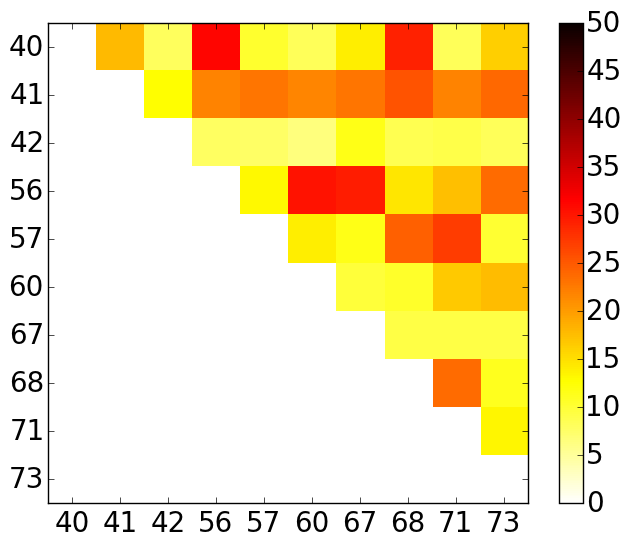
\includegraphics[width=35mm]{Chapters/05_Separation_Known/figures/PEASSplots/OPS/NMF2.png} & 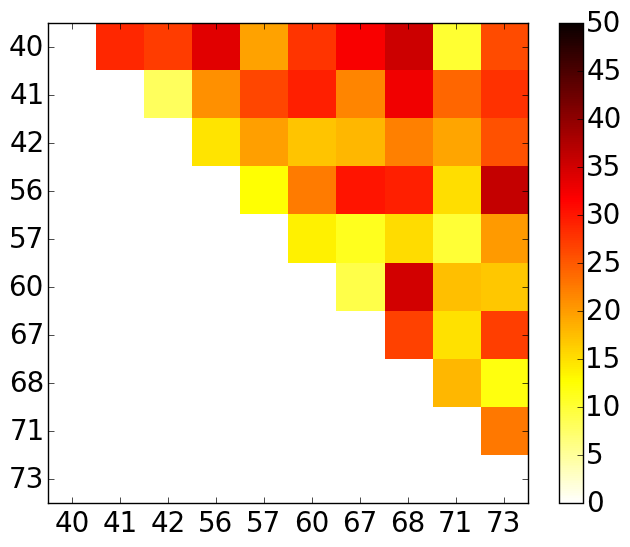
\includegraphics[width=35mm]{Chapters/05_Separation_Known/figures/PEASSplots/OPS/NMF4.png} \\
%     (a) NMF $K=2$ & (b) NMF $K=4$ \\[6pt]
%         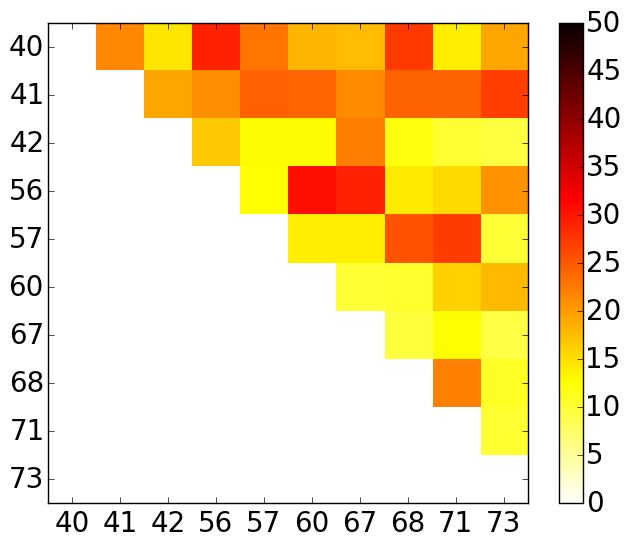
\includegraphics[width=35mm]{Chapters/05_Separation_Known/figures/PEASSplots/OPS/NMFWARP2.png} & 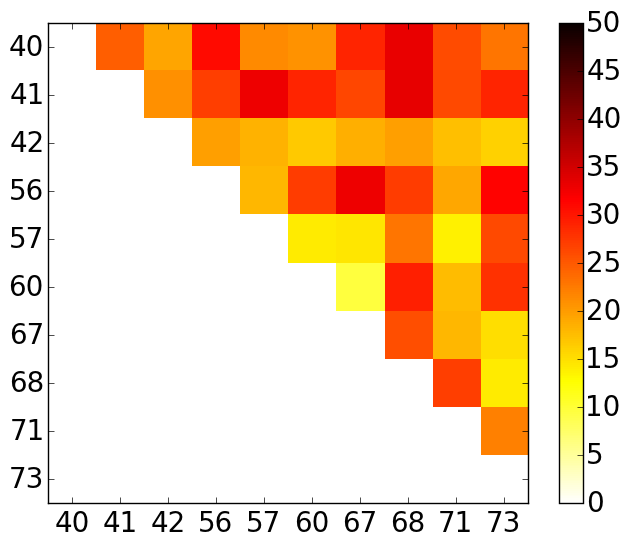
\includegraphics[width=35mm]{Chapters/05_Separation_Known/figures/PEASSplots/OPS/NMFWARP4.png} \\
%     (c) PVI-NMF $K=2$ & (d) PVI-NMF $K=4$ \\[6pt]
%          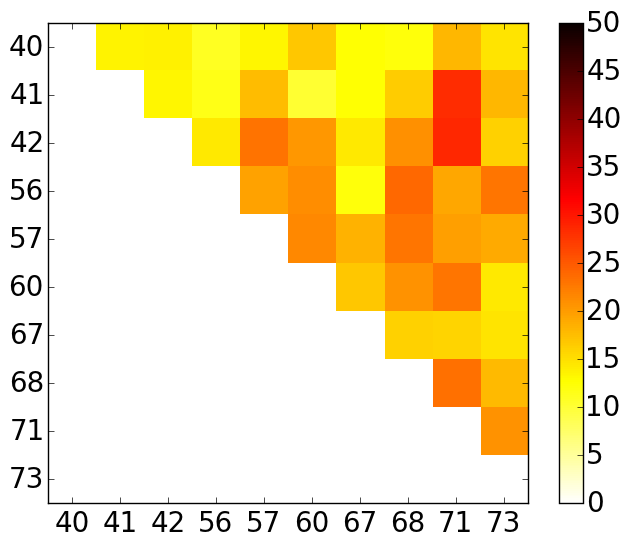
\includegraphics[width=35mm]{Chapters/05_Separation_Known/figures/PEASSplots/OPS/NTF2.png} & 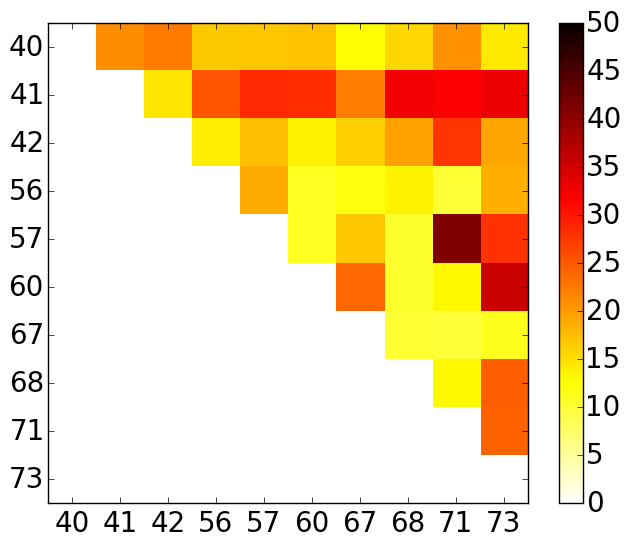
\includegraphics[width=35mm]{Chapters/05_Separation_Known/figures/PEASSplots/OPS/NTF4.png} \\
%     (e) MOD-NTF $K=2$ & (f) MOD-NTF $K=4$ \\[6pt]
% \end{tabular}
% \caption{Results of Overall Perceptual Score. Each matrix represents the mean OPS values for each individual mixture of two sources. The x and y axis represent the instrument IDs in General MIDI notation (See Table~\ref{tab:testset}).}
% \label{tab:resultsmatrix}
% \end{center}

% \end{figure}

% TODO
% \begin{figure}[H]
%     \centering
%     \tiny
%     \subfloat[Source 1]{
%         \begin{tikzpicture}
%             \begin{axis}[mystyle]
%             \addplot [forget plot] graphics [xmin=0.5,xmax=1121.5,ymin=0.5,ymax=273.5] {Chapters/05_Separation_Known/figures/src1-1.png};
%             \end{axis}
%         \end{tikzpicture}%
%     }\hfill
%     \subfloat[Source 2]{
%         \begin{tikzpicture}
%             \begin{axis}[mystyle]
%             \addplot [forget plot] graphics [xmin=0.5,xmax=1121.5,ymin=0.5,ymax=273.5] {Chapters/05_Separation_Known/figures/src2-1.png};
%             \end{axis}
%         \end{tikzpicture}%
%     }
%
%     \subfloat[Mixture]{
%         \begin{tikzpicture}
%             \begin{axis}[mystyle]
%             \addplot [forget plot] graphics [xmin=0.5,xmax=1121.5,ymin=0.5,ymax=273.5] {Chapters/05_Separation_Known/figures/mix-1.png};
%             \end{axis}
%         \end{tikzpicture}%
%     }
%
%     \subfloat[Mix. warped by Pitch 1]{
%         \begin{tikzpicture}
%             \begin{axis}[mystyle]
%             \addplot [forget plot] graphics [xmin=0.5,xmax=1121.5,ymin=0.5,ymax=273.5] {Chapters/05_Separation_Known/figures/mixwrpedsrc1-1.png};
%             \end{axis}
%         \end{tikzpicture}%
%     }\hfill
%     \subfloat[Mix. warped by Pitch 2]{
%         \begin{tikzpicture}
%             \begin{axis}[mystyle]
%             \addplot [forget plot] graphics [xmin=0.5,xmax=1121.5,ymin=0.5,ymax=273.5] {Chapters/05_Separation_Known/figures/mixwrpedsrc2-1.png};
%             \end{axis}
%         \end{tikzpicture}%
%     }
%
%     \subfloat[Target 1 warped]{
%         \begin{tikzpicture}
%             \begin{axis}[mystyle]
%             \addplot [forget plot] graphics [xmin=0.5,xmax=1121.5,ymin=0.5,ymax=273.5] {Chapters/05_Separation_Known/figures/src1wrped-1.png};
%             \end{axis}
%         \end{tikzpicture}%
%     }\hfill
%     \subfloat[Target 2 warped]{
%         \begin{tikzpicture}
%             \begin{axis}[mystyle]
%             \addplot [forget plot] graphics [xmin=0.5,xmax=1121.5,ymin=0.5,ymax=273.5] {Chapters/05_Separation_Known/figures/src2wrped-1.png};
%             \end{axis}
%         \end{tikzpicture}%
%     }
%
%     \subfloat[Target 1 unwarped]{
%         \begin{tikzpicture}
%             \begin{axis}[mystyle]
%             \addplot [forget plot] graphics [xmin=0.5,xmax=1121.5,ymin=0.5,ymax=273.5] {Chapters/05_Separation_Known/figures/src1unwarped-1.png};
%             \end{axis}
%         \end{tikzpicture}%
%     }\hfill
%     \subfloat[Target 2 unwarped]{
%         \begin{tikzpicture}
%             \begin{axis}[mystyle]
%             \addplot [forget plot] graphics [xmin=0.5,xmax=1121.5,ymin=0.5,ymax=273.5] {Chapters/05_Separation_Known/figures/src2unwarped-1.png};
%             \end{axis}
%         \end{tikzpicture}%
%     }
%     \caption{Example of pitch variation informed NMF in the warped domain. \textit{Time} is shown on horizontal axes. \textit{Frequency} is shown on vertical axes.}
%     \label{fig:warpingdemo}
% \end{figure}

\section{Extending Pitch Variation Informed Separation}

\marginpar{This results of this extension were submitted and evaluated in SiSEC 2015 and SiSEC 2016.}

In the previous section, we showed the effectiveness of a pitch variation informed separation system on our constrained unison source separation scenario.
In the following section I show how the method can be extended to the scenario of separating the vocals/lead from the accompaniment in professionally produced music.

% from zafar
Hereby I make use of one particularity of harmonic lead sources like singing voice.
It is their ability to produce vibration using vocal folds, further filtered by the vocal tract.
As a consequence, sung melodies are \textit{mostly} harmonic and therefore have a fundamental frequency.
If one can track the pitch of the vocals, one can then estimate the energy at the harmonics of the fundamental frequency and reconstruct the voice.

Such method is summarized in Figure~\ref{fig:methods_harmonicity}.
In a first step, the objective is to get estimates of the time-varying fundamental frequency for the lead at each time frame.
This can done by a suitable pitch detection method like~\cite{de2002yin}.
A second step then is respect is then to track this fundamental frequency over time, in other words, to find the best sequence of estimates, in order to identify the melody line.
Such algorithms typically assume that the lead corresponds to the harmonic signal with strongest amplitude.
In this extension, I want show how the pitch variation informed separation system can be used in combination with a predominant melody estimation algorithm to extract singing voice from music.
\par
In a first step, the ``Melodia'' algorithm~\cite{salamon12} is used to obtain an estimate of the predominant melody from the mixture.
The mixture is then time warped based on the fundamental frequency of the melody so that it’s predominant solo part is nearly constant in F0. (See~\cite{salamon12} for details). The extraction is then carried out in time domain using efficient comb filtering.

\begin{figure}[htbp]
	\centering
  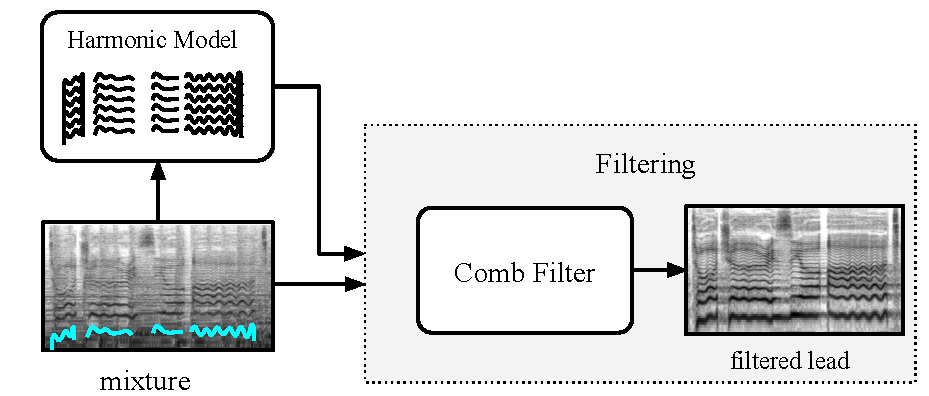
\includegraphics[width=\columnwidth]{Chapters/05_Separation_Known/figures/comb_filter.pdf}
	\caption{Block scheme diagram of a \textit{harmonic assumption} for vocals. In a first analysis step, the fundamental frequency of the lead signal is extracted. From it, a separation is obtained by filtering the mixture.}
	\label{fig:methods_harmonicity}
\end{figure}

\subsection{Predominant Melody Estimation}

% TODO:  add phd thesis from justin: ~\cite{salamon13}
The first step to extend the pitch variation informed separation system is to obtain a warp contour that follows the predominant source by means of extraction from the mixture (blind) or by human annotation (informed).
In the following I want to focus how to obtain such a warp contour using a predominant melody algorithm.\par

Estimating the fundamental frequency of one single source from a mixture of several sources is considered very difficult~\cite{klapuri08}.
However, in the case of vocal/accompaniment separation, we only consider one single source is considered as the lead source - usually the vocals.
This assumption often is applicable in modern popular music where such a lead source often is mixed louder than the other sources in the mix.
\par
Now, extracting the lead pitch contour is actually an ongoing field of research named ``melody estimation''.
However, compared to pitch or fundamental frequency, the term ``melody'' line  is only loosely defined.
A widely used defintion is the one from~\cite{poliner07}:

\begin{quote}
  ``...melody is the single (monophonic) pitch sequence that a listener might reproduce if asked to whistle or hum a piece of polyphonic music, and that a listener would recognize as being the `essence` of that music when heard in comparison.''
\end{quote}

For a more comprehensive overview of melody extraction methods, the reader is referred to~\cite{salamon14}.
In this work, I follow the ``Understanding without Separation'' paradigm, which is seen as an advantage of a melody extraction method without applying a source separation system first (also see Chapter 1, Section 1.4.5~\cite{salamon14}).\par

In turn I used the \emph{Melodia} algorithm, published by Salamon et al. in 2012~\cite{salamon12} as the basis to extract vocals from the mixture.\par

\emph{Melodia} consists of four parts:
\noindent\textbf{1)}: a time-frequency transformation is applied and spectral peaks are extracted.
\textbf{2)}: these form the basis of a \emph{saliency} spectrogram that is computed using a weighted sum over all frequencies. This allows emphasize the predominant/salient frequencies in the signal and is the core part of the \emph{Melodia} algorithm.
\textbf{3)}: From the saliency map, again, peaks are extracted and then connected to a melody line. This would already a good starting point for the melody estimate but usually contains way to many outliers due to the noisiness of the saliency representation.
\textbf{4)}: The melody line is post-processed using a viterbi decoder.
The purpose of it is to filter the contour by removing outliers, octave jumps and generally improves the smoothness of the contour using a number of heuristics.
It is important to note that this step is tracking the melody line of the previous step over time.
Usually this step is sensitive to the overall length of the processed mixture and often, this step is computed in a semantically meaningful segment of the mixture like a full track or a refrain.
\par
I applied the \emph{Melodia} using the implementation in Essentia~\cite{bogdanov13} with the default parameters (sample rate 22050 Hz, hop size = 3 ms, window size=46 ms).

\subsection{Source Extraction using Time Warping}

Once the predominant melody is obtained, the warp contour can be computed in the same way as described in Section~\ref{sub:time_warping} above.
In the unison scenario, however, we were globally warping the signal using a continuous warp contour.
In the case of full length tracks many parts are unvoiced and apply time warping on these segments would degrade the separation quality.
Therefore I only applied the warping on voiced parts and leave the non-vocal parts unaltered.
In order to do this, I used the built-in voice activity detection from \emph{Melodia}.
For all continuously voiced segments, I compute the warp contour from the  melody segments.
To reduce the complexity of the extraction, compared to the NMF mentioned in Section~\ref{sub:frequency_modulation}, I designed a comb filter that can extract the voice in the warped time domain.
Therefore I used a simple IIR Filter with the frequency response

\begin{equation}
  H(z) = \frac{1}{1 - 0.75^z{-P}},
\end{equation}

where \(P\) is constant --- due to the time warping --- pitch period in samples.
In order to then extract the vocals, zero-phase filtering is applied.
The extracted vocals were unwarped to linear time and the accompaniment signal is created by subtracting the estimated vocals from the mixture signals.
Each excerpt is then linearly crossfaded into the unaltered, accompaniment/mixture using a 10ms window.
To further reduce the complexity of the separation system, instead one comb filter for each excerpts, I modified the warping algorithm so that a user defined target pitch \(P\), rounded to integer, is used.
That way, the full signal is unwarped and resampled to the same pitch, which then only requires a singe comb filter to extract the signal.
A stereo signal is produced by using a signal filtering both channels individually.

The full procedure is depcited in Figure~\ref{fig:warp_demo}.

\begin{figure}
\begin{tabular}{cc}
  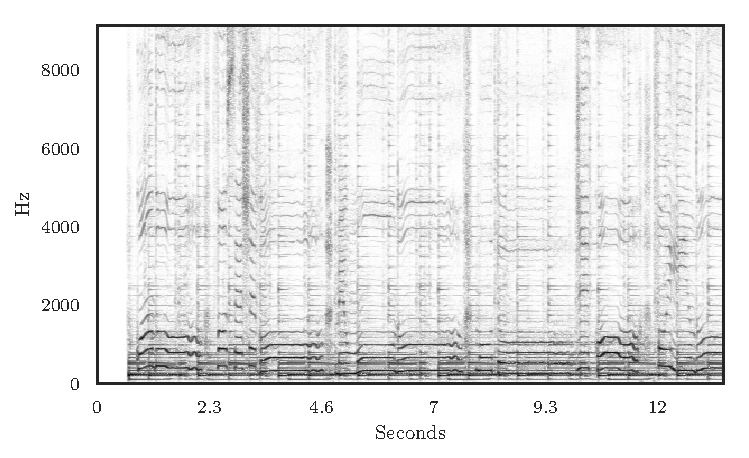
\includegraphics[width=65mm]{Chapters/05_Separation_Known/warp-demo/Mixture.pdf} & 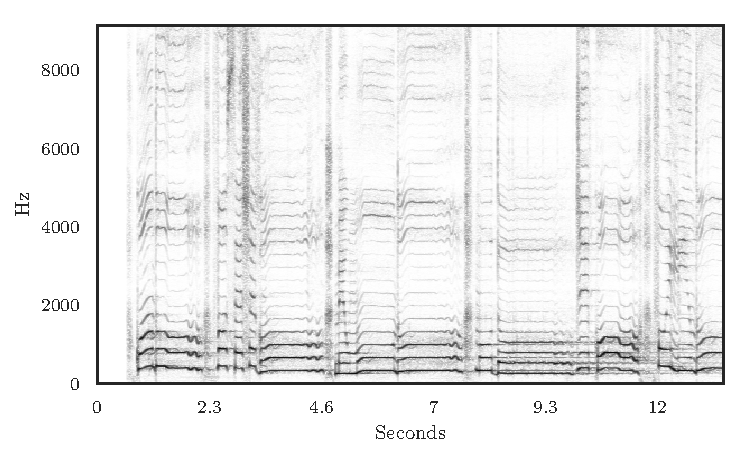
\includegraphics[width=65mm]{Chapters/05_Separation_Known/warp-demo/reference.pdf} \\
(a) Mixture Magnitude STFT & (b) Ground Truth Vocals \\[6pt]
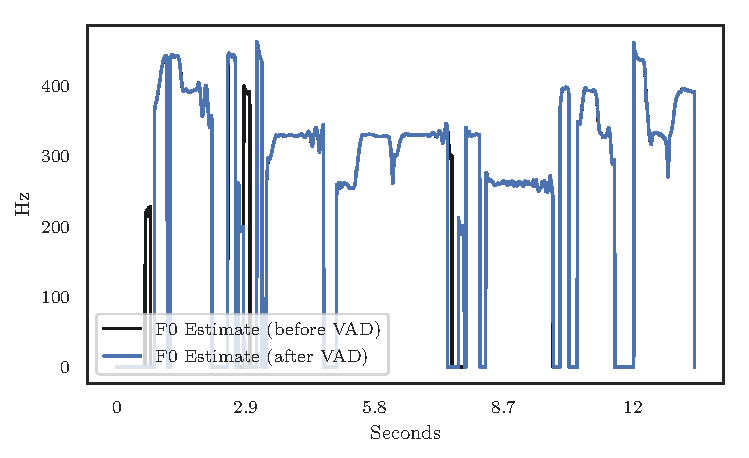
\includegraphics[width=65mm]{Chapters/05_Separation_Known/warp-demo/Melodia.pdf} & 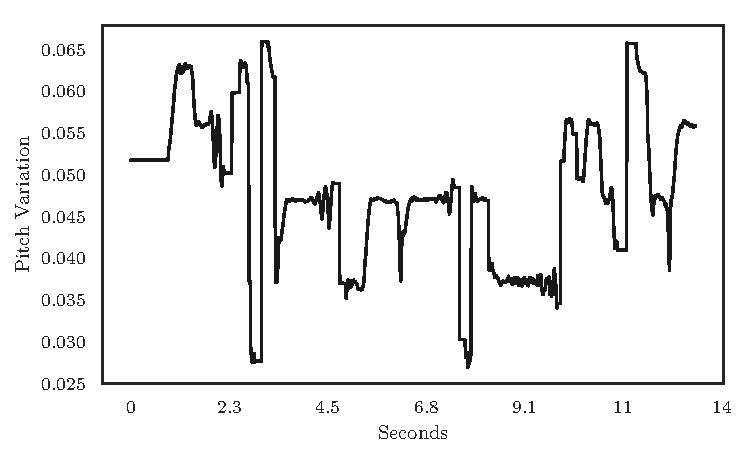
\includegraphics[width=65mm]{Chapters/05_Separation_Known/warp-demo/Contour.pdf} \\
(c) Melody Estimate & (d) Warp Contour \\[6pt]
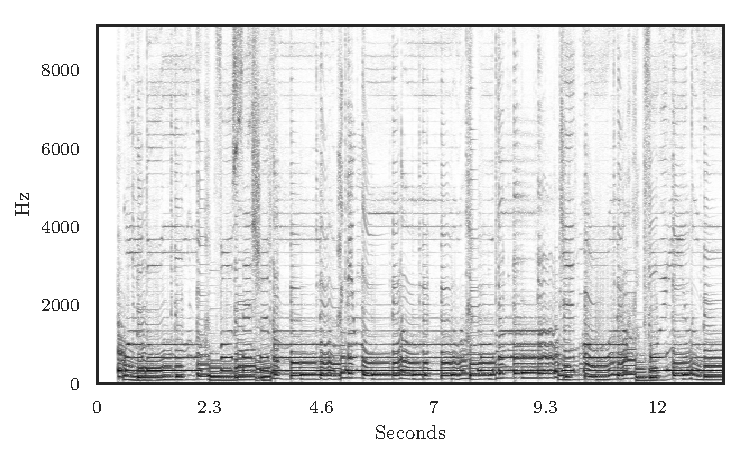
\includegraphics[width=65mm]{Chapters/05_Separation_Known/warp-demo/warped.pdf} & 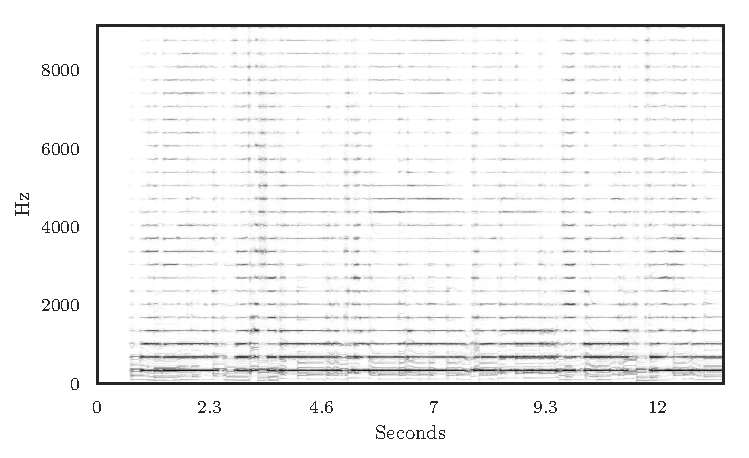
\includegraphics[width=65mm]{Chapters/05_Separation_Known/warp-demo/warped_filtered.pdf} \\
(e) Warped Mixture & (f) Filtered Mixture \\[6pt]
\multicolumn{2}{c}{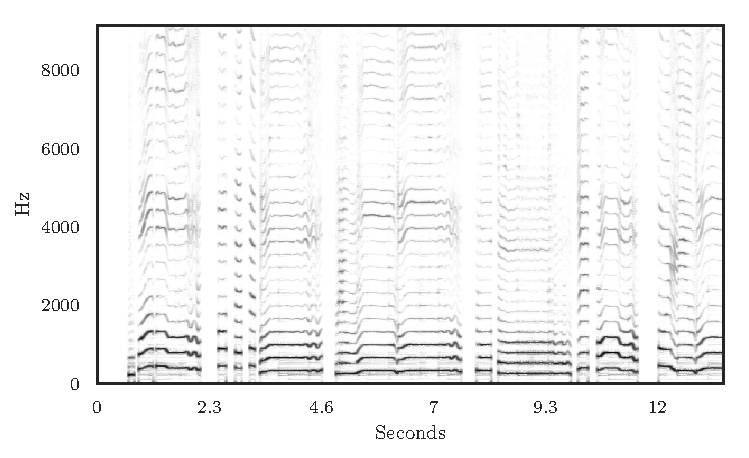
\includegraphics[width=65mm]{Chapters/05_Separation_Known/warp-demo/Estimate.pdf} }\\
\multicolumn{2}{c}{(g) Vocals Estimate}
\end{tabular}
\caption{Examples of a pitch variation informed separation of the audio track \emph{Tamy - Que Pena Tanto Fa}.}%
\label{fig:warp_demo}
\end{figure}

\subsection{Results on SiSEC 2015}
\label{ssec:performance}

The algorithm has been applied to the Mixing Secret Dataset 100 (MSD100) dataset,  consisting of a total of 100 songs of different styles.
The separation results were evaluated using BSSeval~\cite{todo} and submitted to the SiSEC 2015 evaluation challenge~\cite{ono15}.
The system was ranked in the last third of the participants and scored only slightly better than RPCA based methods~\cite{huang12}.
The reason for this is that our proposed system highly depends on the melody estimation algorithm which in turns is based on the assumption that there exist a predominant melody in the mixture.
Unfortunately, the newly created MSD100 dataset was not mixed using professional mastering, resulting in vocals that are below average in loudness.
Due to the small energy, they were not detected as voiced by \emph{Melodia}, hence the warping was either not applied. Even worse, sometimes the pitch estimates were one octave off producing severe artifacts due to extreme warping.\par
On the positive side, the proposed method is of very low complexity and generally implemented in Python and has very low computational complexity.

\subsection{Improving Voiced/Unvoiced Detection using Deep Neural Networks}

As mentioned in the previous section, voice activity detection is of paramount importance in the proposed music separation system.
Therefore, I decided to evaluate if the performance of the system can be improved by using a more robust voice activity detection method as a separate preprocessing step.
\par
Shortly after I submitted the separation results to the SiSEC 2015 evaluation campaign, the whole audio community was shaken up by the recent success of deep learning throughout several audio related tasks that go beyond automatic speech recognition.
Among them are several tasks related to music information retrieval (MIR) such as singing voice detection which received major breakthroughs in 2014 and 2015~\cite{Lehner14, Lehner15, Leglaive15, schlueter15}.
\par
Locking back, at that time, I did not have enough knowledge to understand how and why deep learning method are so successful~\footnote{And even today, very few people would say that the deep learning community made significant progress regarding the understanding of DNNs.}.
Therefore, I decided to deploy a state-of-the-art singing voice detection system into my separation pipeline and evaluate just the end-to-end performance.
I chose to reimplement the system by Leglaive~\cite{Leglaive15}, since it was a good compromise between complexity (its uses hand-crafted features instead of large STFT frames) and performance.
In fact, the system reached a state-of-the-art accuracy of 91.5\% (F-measure of 91.5) for classifying frames of singing voice for the annotated \emph{Jamendo} singing voice detection dataset~\cite{ramona08}, which is an improvement of more than 10\% compared to the best performing non-DNN system.
I want to briefly describe the system published in in~\cite{Leglaive15}, for more details, the reader is referred to the original authors publications.
Also in the course of this thesis more of my work is based on the deep learning framework and will be explained in further details in Chapter~\ref{chapx, chapy}
\par
The method proposed in~\cite{Leglaive15} is based on a recurrent neural network (RNN) layer is very similar to a classical fully connected neural network, except that RNN applies the same set of weights recursively over an input sequence.
RNNs excelt at detecting structure in sequential data of arbitrary length.
This makes it ideal to model time series, however, in practice, the temporal context learnt is limited to only a few time instances, because of the vanishing gradient problem~\cite{Hochreiter98}.
To alleviate this problem, forgetting factors (also called gating) were proposed.
One of the most popular gated recurrent cells is the Long Short-Term Memory (LSTM)~\cite{Hochreiter97} cell.
Its effectiveness has been proven in various applications and LSTMs are the state-of-the-art approach for speech recognition~\cite{Graves13}.
The basic structue of such a sequential network is depicted in Figure~\ref{fig:lstm_2}.
\begin{figure}
  \centering
  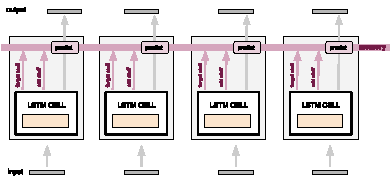
\includegraphics[width=0.8\textwidth]{Chapters/05_Separation_Known/figures/lstm_2.pdf}
  \caption{Simpliefied Block diagram of a Long Short-Term Memory Network.}
  \label{fig:lstm_2}
\end{figure}
The input of the network is a 80 dimensional feature vector consisting of harmonically and percussively enhanced STFT frames of the mixture as described in~\cite{ono08}.
The output of the network is a framewise integer, indicating `1.0` for singing voice and `0.0` for \emph{unvoiced} frames.
I trained the network using a fixed number of frames from the DSD100 training dataset.
The vocal activity labels were obtained from the dataset by analyzing the true vocals.
The network was created and trained using the Keras python framework~\cite{chollet17}.
I stacked up to three layers using the parameters as mentioned in~\cite{Leglaive15} but used unidirectional LSTMs instead of bi-directional to reduce computation complexity.
The trained network achieves an accuracy of 85\% on the separate test set.\par
While the original network proposed in~\cite{leglaive15} was framed as  classification problem, I modified the sigmoid output activation and replaced it with a linear activation to get a linear gain \(g\) instead of probability.
This gain is then multiplied with the mixture signal so that segments with less energy are reduced in volume.
In experiments I found out that this helps the \emph{Melodia} algorithm to better detect vocal activity throughout an audio track and therefore yields in melody estimates with fewer errors.

\begin{figure}
  \centering
  % This file was created by matlab2tikz.
%
%The latest updates can be retrieved from
%  http://www.mathworks.com/matlabcentral/fileexchange/22022-matlab2tikz-matlab2tikz
%where you can also make suggestions and rate matlab2tikz.
%
\begin{tikzpicture}

\begin{axis}[%
width=1.396in,
height=0.78in,
at={(0.57in,3.0in)},
scale only axis,
xmin=0.5,
xmax=2.5,
ymin=-11.8456832139538,
ymax=12.0983588349663,
ylabel style={font=\color{white!15!black}},
ylabel={SDR},
axis background/.style={fill=white},
xticklabels={},
title style={font=\bfseries},
title={vocals},
ymajorgrids,
yminorgrids
]
\addplot [color=black, forget plot]
  table[row sep=crcr]{%
0.6	-1.9758567749213\\
0.6	-1.1472747974891\\
0.6	0.0481517271656759\\
1.4	0.0481517271656759\\
1.4	-1.1472747974891\\
1.4	-1.9758567749213\\
1.4	-2.8044387523535\\
1.4	-3.6836695149443\\
0.6	-3.6836695149443\\
0.6	-2.8044387523535\\
0.6	-1.9758567749213\\
};
\addplot [color=black, forget plot]
  table[row sep=crcr]{%
1.6	-0.507353682851228\\
1.6	0.113338890967634\\
1.6	0.852771078194694\\
2.4	0.852771078194694\\
2.4	0.113338890967634\\
2.4	-0.507353682851228\\
2.4	-1.12804625667009\\
2.4	-1.94274438664256\\
1.6	-1.94274438664256\\
1.6	-1.12804625667009\\
1.6	-0.507353682851228\\
};
\addplot [color=black, forget plot]
  table[row sep=crcr]{%
1	-6.78225690045683\\
1	-3.6836695149443\\
};
\addplot [color=black, forget plot]
  table[row sep=crcr]{%
2	-4.92374070693745\\
2	-1.94274438664256\\
};
\addplot [color=black, forget plot]
  table[row sep=crcr]{%
1	2.55938991049521\\
1	0.0481517271656759\\
};
\addplot [color=black, forget plot]
  table[row sep=crcr]{%
2	2.42428921907715\\
2	0.852771078194694\\
};
\addplot [color=black, forget plot]
  table[row sep=crcr]{%
0.95	-6.78225690045683\\
1.05	-6.78225690045683\\
};
\addplot [color=black, forget plot]
  table[row sep=crcr]{%
1.95	-4.92374070693745\\
2.05	-4.92374070693745\\
};
\addplot [color=black, forget plot]
  table[row sep=crcr]{%
0.95	2.55938991049521\\
1.05	2.55938991049521\\
};
\addplot [color=black, forget plot]
  table[row sep=crcr]{%
1.95	2.42428921907715\\
2.05	2.42428921907715\\
};
\addplot [color=CTlink, forget plot]
  table[row sep=crcr]{%
0.6	-1.9758567749213\\
1.4	-1.9758567749213\\
};
\addplot [color=CTlink, forget plot]
  table[row sep=crcr]{%
1.6	-0.507353682851228\\
2.4	-0.507353682851228\\
};
\addplot [color=CTlink, draw=none, mark=+, mark options={solid, CTlink}, forget plot]
  table[row sep=crcr]{%
1	-14.3959348646932\\
1	-9.54992631980009\\
2	-8.26993351147881\\
};
\addplot [color=CTlink, draw=none, mark=o, mark options={solid, CTlink}, forget plot]
  table[row sep=crcr]{%
2	-11.9927544705679\\
};
\node[above, align=center, font=\color{CTlink}]
at (axis cs:1.25,0.058) {-2.0};
\node[above, align=center, font=\color{CTlink}]
at (axis cs:2.25,0.858) {-0.5};
\end{axis}

\begin{axis}[%
width=1.396in,
height=0.78in,
at={(0.57in,2in)},
scale only axis,
xmin=0.5,
xmax=2.5,
ymin=-3.96838110928441,
ymax=33.8051471982415,
ylabel style={font=\color{white!15!black}},
ylabel={ISR},
axis background/.style={fill=white},
title style={font=\bfseries},
xticklabels={},
xmajorgrids,
xminorgrids,
ymajorgrids,
yminorgrids
]
\addplot [color=black, forget plot]
  table[row sep=crcr]{%
0.6	3.50620881354056\\
0.6	4.05770869257335\\
0.6	4.44397637616963\\
1.4	4.44397637616963\\
1.4	4.05770869257335\\
1.4	3.50620881354056\\
1.4	2.95470893450776\\
1.4	1.96009545714002\\
0.6	1.96009545714002\\
0.6	2.95470893450776\\
0.6	3.50620881354056\\
};
\addplot [color=black, forget plot]
  table[row sep=crcr]{%
1.6	2.14304180047585\\
1.6	2.51961815215558\\
1.6	2.90572551289987\\
2.4	2.90572551289987\\
2.4	2.51961815215558\\
2.4	2.14304180047585\\
2.4	1.76646544879613\\
2.4	1.20967651986024\\
1.6	1.20967651986024\\
1.6	1.76646544879613\\
1.6	2.14304180047585\\
};
\addplot [color=black, forget plot]
  table[row sep=crcr]{%
1	-0.40174698709892\\
1	1.96009545714002\\
};
\addplot [color=black, forget plot]
  table[row sep=crcr]{%
2	-0.482277241947297\\
2	1.20967651986024\\
};
\addplot [color=black, forget plot]
  table[row sep=crcr]{%
1	7.91643810164209\\
1	4.44397637616963\\
};
\addplot [color=black, forget plot]
  table[row sep=crcr]{%
2	4.97064159442628\\
2	2.90572551289987\\
};
\addplot [color=black, forget plot]
  table[row sep=crcr]{%
0.95	-0.40174698709892\\
1.05	-0.40174698709892\\
};
\addplot [color=black, forget plot]
  table[row sep=crcr]{%
1.95	-0.482277241947297\\
2.05	-0.482277241947297\\
};
\addplot [color=black, forget plot]
  table[row sep=crcr]{%
0.95	7.91643810164209\\
1.05	7.91643810164209\\
};
\addplot [color=black, forget plot]
  table[row sep=crcr]{%
1.95	4.97064159442628\\
2.05	4.97064159442628\\
};
\addplot [color=CTlink, forget plot]
  table[row sep=crcr]{%
0.6	3.50620881354056\\
1.4	3.50620881354056\\
};
\addplot [color=CTlink, forget plot]
  table[row sep=crcr]{%
1.6	2.14304180047585\\
2.4	2.14304180047585\\
};
\addplot [color=CTlink, draw=none, mark=+, mark options={solid, CTlink}, forget plot]
  table[row sep=crcr]{%
1	-3.28408406277023\\
2	6.397293668273\\
2	7.20875679699654\\
2	-2.83798717487847\\
};
\node[above, align=center, font=\color{CTlink}]
at (axis cs:1.25,4.47) {3.5};
\node[above, align=center, font=\color{CTlink}]
at (axis cs:2.25,2.959) {2.1};
\end{axis}

\begin{axis}[%
width=1.396in,
height=0.78in,
at={(0.57in,1in)},
scale only axis,
xmin=0.5,
xmax=2.5,
ymin=-24.6956290240449,
ymax=20.9072423316779,
ylabel style={font=\color{white!15!black}},
ylabel={SIR},
axis background/.style={fill=white},
title style={font=\bfseries},
xticklabels={},
xmajorgrids,
xminorgrids,
ymajorgrids,
yminorgrids
]
\addplot [color=black, forget plot]
  table[row sep=crcr]{%
0.6	-2.48453261782208\\
0.6	-0.3132784539727\\
0.6	2.53580554448196\\
1.4	2.53580554448196\\
1.4	-0.3132784539727\\
1.4	-2.48453261782208\\
1.4	-4.65578678167146\\
1.4	-7.24322976085196\\
0.6	-7.24322976085196\\
0.6	-4.65578678167146\\
0.6	-2.48453261782208\\
};
\addplot [color=black, forget plot]
  table[row sep=crcr]{%
1.6	-2.48758804804584\\
1.6	-0.324985030085506\\
1.6	2.51267739901011\\
2.4	2.51267739901011\\
2.4	-0.324985030085506\\
2.4	-2.48758804804584\\
2.4	-4.65019106600618\\
2.4	-7.22739431445643\\
1.6	-7.22739431445643\\
1.6	-4.65019106600618\\
1.6	-2.48758804804584\\
};
\addplot [color=black, forget plot]
  table[row sep=crcr]{%
1	-20.2011258746078\\
1	-7.24322976085196\\
};
\addplot [color=black, forget plot]
  table[row sep=crcr]{%
2	-18.5324438120827\\
2	-7.22739431445643\\
};
\addplot [color=black, forget plot]
  table[row sep=crcr]{%
1	13.5361423309813\\
1	2.53580554448196\\
};
\addplot [color=black, forget plot]
  table[row sep=crcr]{%
2	12.314299783158\\
2	2.51267739901011\\
};
\addplot [color=black, forget plot]
  table[row sep=crcr]{%
0.95	-20.2011258746078\\
1.05	-20.2011258746078\\
};
\addplot [color=black, forget plot]
  table[row sep=crcr]{%
1.95	-18.5324438120827\\
2.05	-18.5324438120827\\
};
\addplot [color=black, forget plot]
  table[row sep=crcr]{%
0.95	13.5361423309813\\
1.05	13.5361423309813\\
};
\addplot [color=black, forget plot]
  table[row sep=crcr]{%
1.95	12.314299783158\\
2.05	12.314299783158\\
};
\addplot [color=CTlink, forget plot]
  table[row sep=crcr]{%
0.6	-2.48453261782208\\
1.4	-2.48453261782208\\
};
\addplot [color=CTlink, forget plot]
  table[row sep=crcr]{%
1.6	-2.48758804804584\\
2.4	-2.48758804804584\\
};
\node[above, align=center, font=\color{CTlink}]
at (axis cs:1.25,2.587) {-2.5};
\node[above, align=center, font=\color{CTlink}]
at (axis cs:2.25,2.528) {-2.5};
\end{axis}

\begin{axis}[%
width=1.396in,
height=0.78in,
at={(0.57in,0.0in)},
scale only axis,
xmin=0.5,
xmax=2.5,
ymin=-9.33793882104533,
ymax=19.711869659802,
ylabel style={font=\color{white!15!black}},
ylabel={SAR},
axis background/.style={fill=white},
title style={font=\bfseries},
xticklabels={},
extra x ticks={1, 2},
extra x tick labels={STO, STOD},
xmajorgrids,
xminorgrids,
ymajorgrids,
yminorgrids
]
\addplot [color=black, forget plot]
  table[row sep=crcr]{%
0.6	-1.49008262500965\\
0.6	-0.937140481566175\\
0.6	-0.397036079394241\\
1.4	-0.397036079394241\\
1.4	-0.937140481566175\\
1.4	-1.49008262500965\\
1.4	-2.04302476845313\\
1.4	-2.88741276240511\\
0.6	-2.88741276240511\\
0.6	-2.04302476845313\\
0.6	-1.49008262500965\\
};
\addplot [color=black, forget plot]
  table[row sep=crcr]{%
1.6	-1.92712180362399\\
1.6	-1.51401965317932\\
1.6	-1.28308624281028\\
2.4	-1.28308624281028\\
2.4	-1.51401965317932\\
2.4	-1.92712180362399\\
2.4	-2.34022395406866\\
2.4	-3.14364249696425\\
1.6	-3.14364249696425\\
1.6	-2.34022395406866\\
1.6	-1.92712180362399\\
};
\addplot [color=black, forget plot]
  table[row sep=crcr]{%
1	-6.47916647615166\\
1	-2.88741276240511\\
};
\addplot [color=black, forget plot]
  table[row sep=crcr]{%
2	-5.90482132380423\\
2	-3.14364249696425\\
};
\addplot [color=black, forget plot]
  table[row sep=crcr]{%
1	2.22561651276376\\
1	-0.397036079394241\\
};
\addplot [color=black, forget plot]
  table[row sep=crcr]{%
2	0.754545016067411\\
2	-1.28308624281028\\
};
\addplot [color=black, forget plot]
  table[row sep=crcr]{%
0.95	-6.47916647615166\\
1.05	-6.47916647615166\\
};
\addplot [color=black, forget plot]
  table[row sep=crcr]{%
1.95	-5.90482132380423\\
2.05	-5.90482132380423\\
};
\addplot [color=black, forget plot]
  table[row sep=crcr]{%
0.95	2.22561651276376\\
1.05	2.22561651276376\\
};
\addplot [color=black, forget plot]
  table[row sep=crcr]{%
1.95	0.754545016067411\\
2.05	0.754545016067411\\
};
\addplot [color=CTlink, forget plot]
  table[row sep=crcr]{%
0.6	-1.49008262500965\\
1.4	-1.49008262500965\\
};
\addplot [color=CTlink, forget plot]
  table[row sep=crcr]{%
1.6	-1.92712180362399\\
2.4	-1.92712180362399\\
};
\addplot [color=CTlink, draw=none, mark=+, mark options={solid, CTlink}, forget plot]
  table[row sep=crcr]{%
1	6.98498144484663\\
2	-7.11676805264549\\
2	-6.06944522075845\\
2	1.8857615511021\\
2	-6.78832410475883\\
2	3.48218878687135\\
};
\node[above, align=center, font=\color{CTlink}]
at (axis cs:1.25,-0.373) {-1.5};
\node[above, align=center, font=\color{CTlink}]
at (axis cs:2.25,-1.272) {-1.9};
\end{axis}

\begin{axis}[%
width=1.396in,
height=0.78in,
at={(2.571in,3in)},
scale only axis,
xmin=0.5,
xmax=2.5,
ymin=-11.8456832139538,
ymax=12.0983588349663,
ylabel style={font=\color{white!15!black}},
ylabel={SDR},
axis background/.style={fill=white},
title style={font=\bfseries},
title={accompaniment},
xticklabels={},
xmajorgrids,
xminorgrids,
ymajorgrids,
yminorgrids
]
\addplot [color=black, forget plot]
  table[row sep=crcr]{%
0.6	4.07993386412816\\
0.6	4.5571974306502\\
0.6	5.62931832744247\\
1.4	5.62931832744247\\
1.4	4.5571974306502\\
1.4	4.07993386412816\\
1.4	3.60267029760612\\
1.4	3.4797877267991\\
0.6	3.4797877267991\\
0.6	3.60267029760612\\
0.6	4.07993386412816\\
};
\addplot [color=black, forget plot]
  table[row sep=crcr]{%
1.6	5.71965452157484\\
1.6	6.33294034116551\\
1.6	7.02863101460487\\
2.4	7.02863101460487\\
2.4	6.33294034116551\\
2.4	5.71965452157484\\
2.4	5.10636870198416\\
2.4	4.26647456977611\\
1.6	4.26647456977611\\
1.6	5.10636870198416\\
1.6	5.71965452157484\\
};
\addplot [color=black, forget plot]
  table[row sep=crcr]{%
1	0.944593194955716\\
1	3.4797877267991\\
};
\addplot [color=black, forget plot]
  table[row sep=crcr]{%
2	2.47249259717672\\
2	4.26647456977611\\
};
\addplot [color=black, forget plot]
  table[row sep=crcr]{%
1	7.86830964455784\\
1	5.62931832744247\\
};
\addplot [color=black, forget plot]
  table[row sep=crcr]{%
2	9.53990054010412\\
2	7.02863101460487\\
};
\addplot [color=black, forget plot]
  table[row sep=crcr]{%
0.95	0.944593194955716\\
1.05	0.944593194955716\\
};
\addplot [color=black, forget plot]
  table[row sep=crcr]{%
1.95	2.47249259717672\\
2.05	2.47249259717672\\
};
\addplot [color=black, forget plot]
  table[row sep=crcr]{%
0.95	7.86830964455784\\
1.05	7.86830964455784\\
};
\addplot [color=black, forget plot]
  table[row sep=crcr]{%
1.95	9.53990054010412\\
2.05	9.53990054010412\\
};
\addplot [color=CTlink, forget plot]
  table[row sep=crcr]{%
0.6	4.07993386412816\\
1.4	4.07993386412816\\
};
\addplot [color=CTlink, forget plot]
  table[row sep=crcr]{%
1.6	5.71965452157484\\
2.4	5.71965452157484\\
};
\addplot [color=CTlink, draw=none, mark=+, mark options={solid, CTlink}, forget plot]
  table[row sep=crcr]{%
2	11.2995823151338\\
};
\node[above, align=center, font=\color{CTlink}]
at (axis cs:1.25,5.689) {4.1};
\node[above, align=center, font=\color{CTlink}]
at (axis cs:2.25,7.072) {5.7};
\end{axis}

\begin{axis}[%
width=1.396in,
height=0.78in,
at={(2.571in,2in)},
scale only axis,
xmin=0.5,
xmax=2.5,
ymin=-3.96838110928441,
ymax=33.8051471982415,
ylabel style={font=\color{white!15!black}},
ylabel={ISR},
axis background/.style={fill=white},
title style={font=\bfseries},
xticklabels={},
xmajorgrids,
xminorgrids,
ymajorgrids,
yminorgrids
]
\addplot [color=black, forget plot]
  table[row sep=crcr]{%
0.6	14.1846658645635\\
0.6	14.9939408596737\\
0.6	15.6697782504659\\
1.4	15.6697782504659\\
1.4	14.9939408596737\\
1.4	14.1846658645635\\
1.4	13.3753908694533\\
1.4	12.0249130473631\\
0.6	12.0249130473631\\
0.6	13.3753908694533\\
0.6	14.1846658645635\\
};
\addplot [color=black, forget plot]
  table[row sep=crcr]{%
1.6	18.0632858964916\\
1.6	19.2169237215004\\
1.6	20.2624022975336\\
2.4	20.2624022975336\\
2.4	19.2169237215004\\
2.4	18.0632858964916\\
2.4	16.9096480714828\\
2.4	15.066573449782\\
1.6	15.066573449782\\
1.6	16.9096480714828\\
1.6	18.0632858964916\\
};
\addplot [color=black, forget plot]
  table[row sep=crcr]{%
1	7.41703006231415\\
1	12.0249130473631\\
};
\addplot [color=black, forget plot]
  table[row sep=crcr]{%
2	10.6448624248896\\
2	15.066573449782\\
};
\addplot [color=black, forget plot]
  table[row sep=crcr]{%
1	19.4650732883217\\
1	15.6697782504659\\
};
\addplot [color=black, forget plot]
  table[row sep=crcr]{%
2	27.7268965181242\\
2	20.2624022975336\\
};
\addplot [color=black, forget plot]
  table[row sep=crcr]{%
0.95	7.41703006231415\\
1.05	7.41703006231415\\
};
\addplot [color=black, forget plot]
  table[row sep=crcr]{%
1.95	10.6448624248896\\
2.05	10.6448624248896\\
};
\addplot [color=black, forget plot]
  table[row sep=crcr]{%
0.95	19.4650732883217\\
1.05	19.4650732883217\\
};
\addplot [color=black, forget plot]
  table[row sep=crcr]{%
1.95	27.7268965181242\\
2.05	27.7268965181242\\
};
\addplot [color=CTlink, forget plot]
  table[row sep=crcr]{%
0.6	14.1846658645635\\
1.4	14.1846658645635\\
};
\addplot [color=CTlink, forget plot]
  table[row sep=crcr]{%
1.6	18.0632858964916\\
2.4	18.0632858964916\\
};
\addplot [color=CTlink, draw=none, mark=+, mark options={solid, CTlink}, forget plot]
  table[row sep=crcr]{%
1	21.401905071888\\
1	2.74498453261405\\
1	21.9336226665764\\
2	6.88346229505207\\
};
\node[above, align=center, font=\color{CTlink}]
at (axis cs:1.25,15.812) {14.2};
\node[above, align=center, font=\color{CTlink}]
at (axis cs:2.25,20.342) {18.1};
\end{axis}

\begin{axis}[%
width=1.396in,
height=0.78in,
at={(2.571in,1in)},
scale only axis,
xmin=0.5,
xmax=2.5,
ymin=-24.6956290240449,
ymax=20.9072423316779,
ylabel style={font=\color{white!15!black}},
ylabel={SIR},
axis background/.style={fill=white},
xticklabels={},
title style={font=\bfseries},
xmajorgrids,
xminorgrids,
ymajorgrids,
yminorgrids
]
\addplot [color=black, forget plot]
  table[row sep=crcr]{%
0.6	8.39513700131584\\
0.6	9.26439178676195\\
0.6	10.033272550563\\
1.4	10.033272550563\\
1.4	9.26439178676195\\
1.4	8.39513700131584\\
1.4	7.52588221586974\\
1.4	6.11826647815662\\
0.6	6.11826647815662\\
0.6	7.52588221586974\\
0.6	8.39513700131584\\
};
\addplot [color=black, forget plot]
  table[row sep=crcr]{%
1.6	7.54419258595698\\
1.6	8.4682930672431\\
1.6	9.60417638684285\\
2.4	9.60417638684285\\
2.4	8.4682930672431\\
2.4	7.54419258595698\\
2.4	6.62009210467087\\
2.4	5.44215271286093\\
1.6	5.44215271286093\\
1.6	6.62009210467087\\
1.6	7.54419258595698\\
};
\addplot [color=black, forget plot]
  table[row sep=crcr]{%
1	0.911564014698467\\
1	6.11826647815662\\
};
\addplot [color=black, forget plot]
  table[row sep=crcr]{%
2	3.09557012359525\\
2	5.44215271286093\\
};
\addplot [color=black, forget plot]
  table[row sep=crcr]{%
1	13.608095186407\\
1	10.033272550563\\
};
\addplot [color=black, forget plot]
  table[row sep=crcr]{%
2	13.8885853596125\\
2	9.60417638684285\\
};
\addplot [color=black, forget plot]
  table[row sep=crcr]{%
0.95	0.911564014698467\\
1.05	0.911564014698467\\
};
\addplot [color=black, forget plot]
  table[row sep=crcr]{%
1.95	3.09557012359525\\
2.05	3.09557012359525\\
};
\addplot [color=black, forget plot]
  table[row sep=crcr]{%
0.95	13.608095186407\\
1.05	13.608095186407\\
};
\addplot [color=black, forget plot]
  table[row sep=crcr]{%
1.95	13.8885853596125\\
2.05	13.8885853596125\\
};
\addplot [color=CTlink, forget plot]
  table[row sep=crcr]{%
0.6	8.39513700131584\\
1.4	8.39513700131584\\
};
\addplot [color=CTlink, forget plot]
  table[row sep=crcr]{%
1.6	7.54419258595698\\
2.4	7.54419258595698\\
};
\node[above, align=center, font=\color{CTlink}]
at (axis cs:1.25,10.06) {8.4};
\node[above, align=center, font=\color{CTlink}]
at (axis cs:2.25,9.614) {7.5};
\end{axis}

\begin{axis}[%
width=1.396in,
height=0.78in,
at={(2.571in,0in)},
scale only axis,
xmin=0.5,
xmax=2.5,
ymin=-9.33793882104533,
ymax=19.711869659802,
ylabel style={font=\color{white!15!black}},
ylabel={SAR},
axis background/.style={fill=white},
title style={font=\bfseries},
xticklabels={},
yticklabels={},
extra x ticks={1, 2},
extra x tick labels={STO, STOD},
xmajorgrids,
xminorgrids,
ymajorgrids,
yminorgrids
]
\addplot [color=black, forget plot]
  table[row sep=crcr]{%
0.6	6.88286322756687\\
0.6	7.33779171661827\\
0.6	7.88948907206887\\
1.4	7.88948907206887\\
1.4	7.33779171661827\\
1.4	6.88286322756687\\
1.4	6.42793473851547\\
1.4	5.84055264173005\\
0.6	5.84055264173005\\
0.6	6.42793473851547\\
0.6	6.88286322756687\\
};
\addplot [color=black, forget plot]
  table[row sep=crcr]{%
1.6	10.7036329091479\\
1.6	11.6159696204354\\
1.6	12.537223176303\\
2.4	12.537223176303\\
2.4	11.6159696204354\\
2.4	10.7036329091479\\
2.4	9.79129619786032\\
2.4	8.4281819325013\\
1.6	8.4281819325013\\
1.6	9.79129619786032\\
1.6	10.7036329091479\\
};
\addplot [color=black, forget plot]
  table[row sep=crcr]{%
1	3.31208622647544\\
1	5.84055264173005\\
};
\addplot [color=black, forget plot]
  table[row sep=crcr]{%
2	5.97129193365591\\
2	8.4281819325013\\
};
\addplot [color=black, forget plot]
  table[row sep=crcr]{%
1	10.6014569969024\\
1	7.88948907206887\\
};
\addplot [color=black, forget plot]
  table[row sep=crcr]{%
2	17.2087716038469\\
2	12.537223176303\\
};
\addplot [color=black, forget plot]
  table[row sep=crcr]{%
0.95	3.31208622647544\\
1.05	3.31208622647544\\
};
\addplot [color=black, forget plot]
  table[row sep=crcr]{%
1.95	5.97129193365591\\
2.05	5.97129193365591\\
};
\addplot [color=black, forget plot]
  table[row sep=crcr]{%
0.95	10.6014569969024\\
1.05	10.6014569969024\\
};
\addplot [color=black, forget plot]
  table[row sep=crcr]{%
1.95	17.2087716038469\\
2.05	17.2087716038469\\
};
\addplot [color=CTlink, forget plot]
  table[row sep=crcr]{%
0.6	6.88286322756687\\
1.4	6.88286322756687\\
};
\addplot [color=CTlink, forget plot]
  table[row sep=crcr]{%
1.6	10.7036329091479\\
2.4	10.7036329091479\\
};
\addplot [color=CTlink, draw=none, mark=+, mark options={solid, CTlink}, forget plot]
  table[row sep=crcr]{%
1	11.2717836172979\\
1	2.55848010624387\\
2	19.2341993371384\\
2	18.9697422641332\\
};
\node[above, align=center, font=\color{CTlink}]
at (axis cs:1.25,7.9) {6.9};
\node[above, align=center, font=\color{CTlink}]
at (axis cs:2.25,12.562) {10.7};
\end{axis}
\end{tikzpicture}%

  \caption{BSS Eval scores for the vocals and accompaniment estimates on the DSD100 dataset as used in~\cite{liutkus17}. Results are shown on the \emph{test} set only. Results indicate the improvements of the DNN based vocal activity detection system.}
  \label{fig:05_comparison_sto_stodnn}
\end{figure}

This DNN-optimized version of the algorithm was then compared (but not submitted) to the new the SiSEC 2016 dataset which was released in the meantime~\cite{liutkus17}.
One can see that the DNN vocal activity dection improved the vocals SDR by 1.5~dB which is considered as a significant improvements.

\section{Excursus: Improving $F0$ Estimation using warped method} % (fold)
\label{sec:method}

\def\ptdbtugsynthYINMEANOMFPE{{0.327}}
\def\ptdbtugsynthYINMEANRMFPE{{0.147}}
\def\ptdbtugsynthYINIMPROMFPE{{55}}
\def\ptdbtugsynthYINSTDOMFPE{{0.214}}
\def\ptdbtugsynthYINSTDRMFPE{{0.214}}
\def\ptdbtugsynthYINTMFPE{{55466}}
\def\ptdbtugsynthYINpMFPE{{.000}}
\def\ptdbtugsynthYINrMFPE{{0.998}}
\def\ptdbtugsynthYINnMFPE{{11487}}
\def\ptdbtugsynthiRAPTMEANOMFPE{{0.434}}
\def\ptdbtugsynthiRAPTMEANRMFPE{{0.138}}
\def\ptdbtugsynthiRAPTIMPROMFPE{{68}}
\def\ptdbtugsynthiRAPTSTDOMFPE{{0.292}}
\def\ptdbtugsynthiRAPTSTDRMFPE{{0.292}}
\def\ptdbtugsynthiRAPTTMFPE{{13831}}
\def\ptdbtugsynthiRAPTpMFPE{{.000}}
\def\ptdbtugsynthiRAPTrMFPE{{1.000}}
\def\ptdbtugsynthiRAPTnMFPE{{11487}}
\def\ptdbtugsynthMELODIAMEANOMFPE{{0.370}}
\def\ptdbtugsynthMELODIAMEANRMFPE{{0.175}}
\def\ptdbtugsynthMELODIAIMPROMFPE{{53}}
\def\ptdbtugsynthMELODIASTDOMFPE{{0.300}}
\def\ptdbtugsynthMELODIASTDRMFPE{{0.300}}
\def\ptdbtugsynthMELODIATMFPE{{12349}}
\def\ptdbtugsynthMELODIApMFPE{{.000}}
\def\ptdbtugsynthMELODIArMFPE{{1.000}}
\def\ptdbtugsynthMELODIAnMFPE{{11487}}
\def\ptdbtugrealYINMEANOMFPE{{0.812}}
\def\ptdbtugrealYINMEANRMFPE{{0.698}}
\def\ptdbtugrealYINIMPROMFPE{{14}}
\def\ptdbtugrealYINSTDOMFPE{{0.804}}
\def\ptdbtugrealYINSTDRMFPE{{0.804}}
\def\ptdbtugrealYINTMFPE{{13082927}}
\def\ptdbtugrealYINpMFPE{{.000}}
\def\ptdbtugrealYINrMFPE{{0.391}}
\def\ptdbtugrealYINnMFPE{{9271}}
\def\ptdbtugrealiRAPTMEANOMFPE{{0.748}}
\def\ptdbtugrealiRAPTMEANRMFPE{{0.744}}
\def\ptdbtugrealiRAPTIMPROMFPE{{1}}
\def\ptdbtugrealiRAPTSTDOMFPE{{0.631}}
\def\ptdbtugrealiRAPTSTDRMFPE{{0.631}}
\def\ptdbtugrealiRAPTTMFPE{{21144487}}
\def\ptdbtugrealiRAPTpMFPE{{.186}}
\def\ptdbtugrealiRAPTrMFPE{{0.016}}
\def\ptdbtugrealiRAPTnMFPE{{9271}}
\def\ptdbtugrealMELODIAMEANOMFPE{{0.677}}
\def\ptdbtugrealMELODIAMEANRMFPE{{0.644}}
\def\ptdbtugrealMELODIAIMPROMFPE{{5}}
\def\ptdbtugrealMELODIASTDOMFPE{{0.784}}
\def\ptdbtugrealMELODIASTDRMFPE{{0.784}}
\def\ptdbtugrealMELODIATMFPE{{20484251}}
\def\ptdbtugrealMELODIApMFPE{{.000}}
\def\ptdbtugrealMELODIArMFPE{{0.047}}
\def\ptdbtugrealMELODIAnMFPE{{9271}}
\def\medleydbMELODIAMEANOMFPE{{1.319}}
\def\medleydbMELODIAMEANRMFPE{{1.194}}
\def\medleydbMELODIAIMPROMFPE{{10}}
\def\medleydbMELODIASTDOMFPE{{1.676}}
\def\medleydbMELODIASTDRMFPE{{1.676}}
\def\medleydbMELODIATMFPE{{134380}}
\def\medleydbMELODIApMFPE{{.000}}
\def\medleydbMELODIArMFPE{{0.517}}
\def\medleydbMELODIAnMFPE{{1055}}
\def\medleydbMELODIAMEANOCORRESTIMATESTEM{{0.869}}
\def\medleydbMELODIAMEANRCORRESTIMATESTEM{{0.876}}
\def\medleydbMELODIAIMPROCORRESTIMATESTEM{{-1}}
\def\medleydbMELODIASTDOCORRESTIMATESTEM{{0.173}}
\def\medleydbMELODIASTDRCORRESTIMATESTEM{{0.173}}
\def\medleydbMELODIATCORRESTIMATESTEM{{124390}}
\def\medleydbMELODIApCORRESTIMATESTEM{{.000}}
\def\medleydbMELODIArCORRESTIMATESTEM{{0.553}}
\def\medleydbMELODIAnCORRESTIMATESTEM{{1055}}


\marginpar{This section is based on the work that has been published in 2015 together with my colleague Nils Werner~\cite{stoeter15icassp}.}

An informed system like the one we described in the previous section often has limitations due to the fact that the provided fundamental frequency variation estimate might not be accurate enough and therefore is subject to an upper limit.
Further, it can be assumed that this upper bound is especially relevant for a warping based system that relies on an instantanous estimation of the fundamental frequency.
\par
Such algorithms for estimating the fundamental frequency ($F0$) of a signal vary in stability and accuracy.
While we developed the framework for a pitch variation informed separation, we found that we can utilize this to also optimize fundamental frequency estimators itself.
In turn, we proposed a method which iteratively improves the estimates of such algorithms by applying in each step a time warp on the input signal based on the previously estimated fundamental frequency.
This time warp is designed to lead to a nearly constant $F0$. A refinement is then calculated through inverse time warping of the result of an $F0$ estimation applied to the warped signal. The proposed refinement algorithm is not limited to specific estimators or optimized for specific input signal characteristics. The method is evaluated on synthetic audio signals as well as speech recordings and polyphonic music recordings. Results indicate a significant improvement on accuracy when using the proposed refinement in combination with several well-known $F0$ estimators

\paragraph{Proposed System}
%
The development of novel methods for fundamental frequency estimation, performing as well as earlier methods, such as the popular correlation based \textsc{YIN} algorithm~\cite{decheveigne02}, has proven challenging.
In a study~\cite{babacan13} it is stated that YIN still performs best in terms of accuracy.
Nevertheless, when using YIN or other block based algorithms, a frame length and a hop size have to be selected trading temporal resolution on one side against frequency accuracy and robustness on the other side.

Especially when the signal is polyphonic, the robustness is the most crucial aspect of a pitch estimator. In work from Mauch et al.~\cite{mauch14}, the robustness of the \textsc{YIN} algorithm is improved by probabilistic post-processing. However, besides robustness, there is a variety of use cases requiring high accuracy as well as high temporal resolution. Application in parametric audio coding~\cite{purnhagen00} requires the parameterization of pitch bends and vibratos. Furthermore, source separation algorithms aiming at the extraction of harmonic sources from the mixture can make use of an instantaneous $F0$ estimate~\cite{virtanen08, stoter14}. There are already contributions addressing the improvement of accuracy of $F0$ estimates such as~\cite{medan91} which introduced a non-integer similarity model or~\cite{christensen07} which belongs to the group of parametric pitch estimators.

We propose to improve the output of already existing algorithms in terms of temporal resolution as well as accuracy by iterative time warping. Two other contributions already make use of time warping in the context of pitch estimation. Resch et al.~\cite{resch07} proposed an instantaneous pitch estimation technique which optimizes a warping function that would lead to a constant pitch signal. Their optimization framework minimizes a cost function specifically targeted for speech signals. Azarov et al.\ have introduced an improved version of RAPT (called iRAPT1 and iRAPT2) which also uses time warping to some extent~\cite{azarov12} but misses an additional step as will be shown in Section~?.
Our main contribution is a time warping based refinement method that is applicable to any F0 estimate. Our method emphasizes the strengths of different estimators and thus can even help to improve their robustness. In the following, we will describe the refinement method (Section~?) and show the experimental evaluation and its results (Section~?).

Depending on the algorithm and application, there are several reasons why $F0$ estimators deliver a less than ideal performance. When the signal tested is not tonal --- like in unvoiced parts of speech --- a proper estimation is impossible. If the estimator is optimized on purely harmonic signals, inharmonicity or frequency jitter of the input signal will increase the estimation error. Many of these reasons will lead to errors on the coarse level of the estimate (like octave jumps). The fine level accuracy is mostly influenced by parameters like time and/or frequency resolution of the estimator. A signal containing rapid changes of the frequency or modulations like ``vibrato'' is therefore more affected regarding fine level error. To obtain a more accurate estimate, we propose to time warp the signal by using the coarse level estimate towards a more constant pitch. The underlying assumption here is that pitch estimators generally perform better the more constant the pitch is.
In this section, we formulate the mathematical background of the time warping and present our proposed method for obtaining a refined $F0$ estimate.

\subsubsection{Initial $F0$ estimate}
\label{ssub:initial_estimate}

The first step is to calculate an initial $F0$ estimate by using an existing pitch estimator. Note that we later require the estimate to be defined for every input sample, thus $\Pitch[n]$ may require interpolation. In our pipeline, we use linear interpolation for all estimators. $F0$ estimators, like YIN~\cite{decheveigne02}, also provide a measure of confidence $c[n]$.
\par
% In the first step, we apply \emph{time warping} which refers to a strictly monotonous mapping
% of the natural or linear time scale $t$ to a warped time scale $\tau$ via a
% mapping function $\tau=w(t)$.
% The mapping between the two domains for the continuous time case then is:
% \begin{equation}\label{eq:contWarpedTime}
% \breve{x}(\tau)=x(w^{-1}(\tau)), \quad x(t)=\breve{x}(w(t))
% \end{equation}
% where $x(t)$ is the linear-time signal and $\breve{x}(\tau)$ is the warped-time signal.
% For the discrete time case, the signals in both linear-time and warped-time domains are sampled
% using a constant sample interval $T$. With sample indices $\nu$ and $n$ for the warped-time domain and linear time-domain respectively, the warping is performed by
%
% \begin{align}
% \breve{x}[\nu] &= x(\sigma[\nu]) & \textrm{ with } & \sigma[\nu] = w^{-1}(\nu T), \\
% \intertext{and the inverse warping by}
% x{}[n] &= \breve{x}(s[n]) & \textrm{ with } & s{}[n] = w(nT).
% \end{align}
%
% \subsubsection{Warp contour}
% \label{subs:warp_contour}

In our application, the warp map $w(t)$ is constructed in such a way that the instantaneous changes in frequency of the signal in the linear time domain are minimized in the warped time domain. For this, we derive the map from an estimate of the fundamental frequency $F0$.

For processing, the actual information needed is not the absolute instantaneous fundamental frequency but only its change over time. This means that the warping contour can be derived from an algorithm which may differ from the actual $F0$ estimator.

The discrete time warp map $w[n]$ is the scaled sum of the relative
frequency contour (the \emph{warp contour}) $W[n]$:
\begin{equation}
w[n]=N \frac{\sum^n_{l=0}{W[l]}}{\sum^{N-1}_{k=0}{W[k]}}  \qquad 0\leq n<N,
\end{equation}
where $N$ being the number of samples of the signal under consideration.
As stated above the full warp map $w(t)$ is then obtained by linearly interpolating $w[n]$. From the requirements for the mapping function it follows that $W[n]$ has to be greater than zero for all $n$. In the case of a perfect $F0$ estimate, the signal warped with the resulting contour would have a constant $F0$ equal to the average $\bar{W}$.

In the scope of this work, the warping is applied globally over the full length of the signals under consideration. An optional confidence measure $c[n]$ can be incorporated for a processed version of the warping contour. This ensures that the warp contour has no discontinuities that result in additional artifacts after re-sampling. If the estimator does not provide such a measure, a separate voiced/unvoiced detection algorithm can be used. To obtain a warp contour $W[n]$ from an $F0$ estimate we propose the following steps: \textbf{(A)} initialize the warp contour with $F0$ estimate $W = \Pitch$, \textbf{(B)} find contour segments with high confidence, i.e. $c[n]$ exceeds a given threshold, \textbf{(C)} linearly connect the high confidence contour segments and \textbf{(D)} set start and end of warp contour to a constant value if confidence is below threshold. That way warping according to $F0$ is applied in the regions of high confidence without significantly affecting the gaps in-between.
\par
To improve the accuracy of the $F0$ estimate, time warping is applied to the input signal $x[n]$ based on $W$. The input signal is 128-times oversampled using sinc based interpolation filters.
From $\breve{x}[n]$ a new $F0$ estimate $\breve{\Pitch_1}[\nu]$ is being calculated as in step \textbf{(A)}. The first step therefore is similar to~\cite{resch}. Additionally, a warped confidence measure $\breve{c}_1[\nu]$ can be used to convert $\breve{\Pitch_1}[\nu]$ into a warped \emph{warp contour} $\breve{W}_1[\nu]$. It is possible to linearly add $\breve{\Pitch_1}[\nu]$ to the first estimate for refinement, as it is done in~\cite{azarov2012instantaneous}. However for linear sweeps, the warped estimate is shifted in time. Thus an error is introduced which is even more distinct if the first $F0$ estimate is error prone. We therefore propose a method to reduce this error:
\begin{itemize}
	\item Inverse time warping is applied to $\breve{\Pitch_1}[\nu]$ based on the original warp contour $W$ resulting in $\Pitch_1[n]$.
	\item A refined $F0$ estimate after one iteration is then calculated by $\Pitch_1^r[n] = \Pitch_1[n] \cdot W[n] / \bar{W}$ assuming that the warp contour is initialized as in step \textbf{(A)} above.
	\item The refinement can be repeated $k$ times to obtain a better estimate. To avoid accumulating errors introduced by the re-sampling based warping, more iterations benefit from calculating a refined warp contour/warp map instead of doing a nested warping on the input signal. The map is obtained by inverse time warping of the warp contour $\breve{W}_1[\nu]$ resulting in $W_1[n]$. A refined warp contour $W_1^r[n]$ is then obtained in the same way as the refined $F0$ estimate is calculated. For the calculation of the $k$th step, time warping is based on the $W_{k-1}^r[n]$ refined warp contour.
\end{itemize}
An example of the proposed refinement is depicted in Figure~\ref{fig:teaser}. The final refined estimate is closer to the reference than the $F0$ estimator without refinement. It also shows (right plot) how much ``flatter'' the $F0$ contour becomes after each iteration.
Note that compared to~\cite{resch}, our method does not use a complex optimisation scheme but relies on the performance of the pitch estimator in successive iterations. Hence our ``black box'' like post processing simplifies the procedure such that it can be applied to any pitch estimator. That way the selection of a pitch estimator which best fits to the signal type can be seen as an optimisation.

\begin{figure}[t]
\centering
\begin{tikzpicture}
\node[inner sep=0pt] (3d) at (4.4,0) {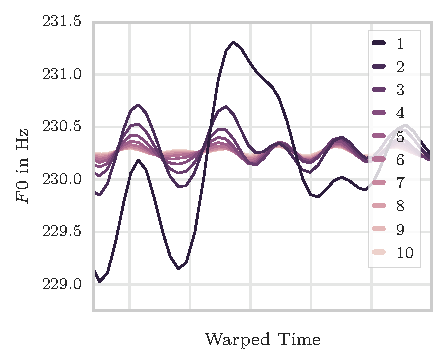
\includegraphics[width=.4\textwidth]{Chapters/05_Separation_Known/figures/f0_3d.pdf}};
\node[inner sep=0pt] (output) at (0,0) {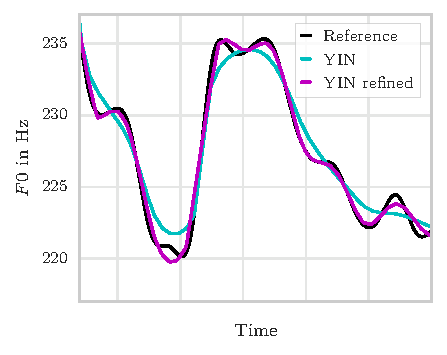
\includegraphics[width=.4\textwidth]{Chapters/05_Separation_Known/figures/output_f0.pdf}};
%
\end{tikzpicture}
\caption{$F0$ refinement for one excerpt of synthesized speech using \textbf{YIN}~\cite{decheveigne02} with 10 iterations. \emph{Left}: Estimated $F0$ in linear time. \emph{Right}: estimates after each warping iteration in warped time.}
\label{fig:teaser}
\end{figure}

\vspace{-0.6em}
\subsection{Experiments and Evaluation} % (fold)
\label{sec:experiments}

For the evaluation of the proposed $F0$ refinement, we test the refinement algorithm with the following $F0$ estimators:\\
\textbf{YIN}~\cite{decheveigne02} is used as an FFT based implementation~\cite{bogdanov13}. The confidence measure is thresholded for values lower than 0.6 on the speech recordings. \textbf{iRAPT1,2}~\cite{azarov12} are improved versions of the RAPT framework. We use the author's MATLAB implementation of the iRAPT1 and iRAPT2 algorithms.\ iRAPT2 is a refinement method that is comparable to our proposed method. To evaluate the results, we apply our refinement to iRAPT1 and compare it with the refinement produced by iRAPT2. $c[n] < 0.7$ is used for thresholding speech recordings. \textbf{MELODIA}~\cite{salamon12} is not designed to be an $F0$ estimator but is able to extract the \emph{predominant} melody in a polyphonic mixture. We increase the bin resolution to 0.5 semitones, to increase the accuracy. We used the \textsc{Essentia} implementation. For thresholding we use the built-in voiced/unvoiced detection.
For YIN and MELODIA, we evaluate on a frame length of 64~ms and a hop size of 16~ms. For iRAPT1 and iRAPT2  we use the fixed frame length parameters of the author's implementation.
\par
We use the established evaluation measures \textsc{Gross Pitch Error} (GPE) and \textsc{Mean Fine Pitch Error} (MFPE)~\cite{azarov12}. We focus on MFPE in our results, measuring the absolute deviation of $F0_{\mathrm{true}}$ and the $F0$ estimate per sample.
As mentioned in~\cite{resch}, evaluating the accuracy of $F0$ estimates is challenging because of the lack of ground truth datasets annotated on a time scale with such a high resolution. Most of the available audio test data sets are not suitable because the $F0$ annotation is only available with low time resolutions. By using such a dataset there is a risk that the refined $F0$ estimate is higher in MFPE. This is because the refined estimates show more of the fine structure deviating from the coarse annotation which then is considered as piecewise constant. To address this issue, we first present the evaluation results on synthetic data. To verify our synthetic results, we present the results of speech data annotated on 10~ms frames derived from laryngograph signals. We did only evaluate and process the voiced parts of the signals as indicated in the provided annotation labels. Also note that since we focus on the MFPE, all segments where one of the estimators results in a GPE $> 0$ are excluded from the results, hence the GPE for all of our results is 0. The proposed refinement has been processed with one iteration ($k=1$). Experiments showed that more iterations only marginally improve the results.

% \vspace{-0.6em}
% \subsubsection{Oracle Refinement}
%
Since the proposed refinement algorithm repeatedly applies pitch estimation, the performance of these estimators on the time warped (nearly constant) signal is of interest. Therefore we included the results of an oracle refinement where the first estimate is set to a ground truth pitch. Additionally this also does reveal information about the quality of the ground truth annotation itself.

\vspace{-0.6em}
\subsubsection{Synthetic Data} % (fold)
\label{ssub:sythetic_data}

To generate synthetic test data we use pitch label annotations of the PTDB-TUG speech data set~\cite{pirker11}. We synthesize the melody or voice using a simple sinusoidal signal model. To get accurate ground truth data, the pitch annotations were up-sampled to audio rate by using linear interpolation for the PTDB-TUG. Similar to~\cite{mauch14}, we then synthesized the data using cosine based oscillators adding 10 harmonics to each signal output.
The test set has been rendered at 16 kHz. The complete PTDB-TUG set results in almost 10 hours of input signal data.
We present the results of the synthetic data as box plots in Figure~\ref{fig:ptdbtug_synth} grouped by estimator. It shows that all estimators benefit from the refinement in terms of MFPE. The iRAPT1 estimator shows the best improvement of \ptdbtugsynthiRAPTIMPROMFPE \% in MFPE. As expected, the Oracle Refinement is almost at 0 MFPE.

\begin{figure}[t!]
\centering
		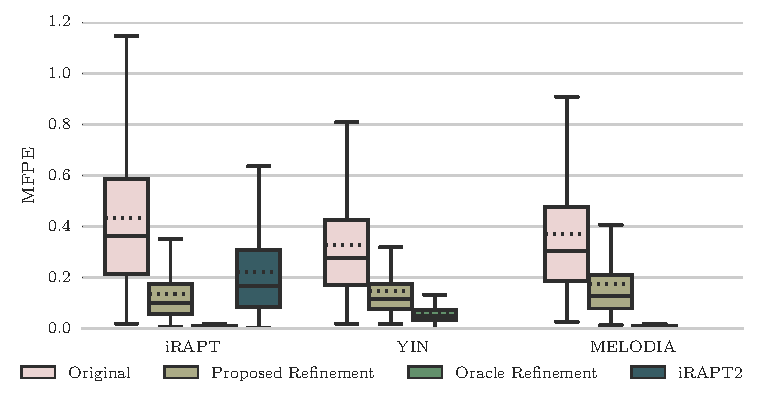
\includegraphics[width=0.90\columnwidth]{Chapters/05_Separation_Known/figures/stats_boxplot_ptdb_synth.pdf}
\caption{Results from the synthesized PTDB-TUG dataset. MFPE grouped by estimator. Solid/dotted lines represent medians/means. Outliers are not shown.}
\label{fig:ptdbtug_synth}
\end{figure}

\vspace{-0.6em}
\subsubsection{Speech Data} % (fold)
\label{ssub:real_data}
For the results of the algorithm on real data we first used the same PTDB-TUG items as in the synthetic data but processed the accompanying speech recordings. The MFPE values were then calculated by averaging the sample wise $F0$ estimates from our proposed method over frame lengths of 10~ms to match the annotation data. The results are shown in Figure~\ref{fig:ptdbtug_real}. The mean values indicate that the MELODIA algorithm performs best overall. We can see that the refinement does not show a clear effect on the iRAPT estimator. The oracle refinement results indicate that even if a ground truth is known, the refinement based on the warped (constant) signal can not get much lower in MFPE. As also seen on synthetic data, iRAPT2 does not show any significant improvements compared to our proposed refinements.

\vspace{-0.6em}
\subsubsection{Polyphonic Mixtures} % (fold)
\label{ssub:real_data}

Pitch estimation of polyphonic mixture input signals in general is known to be more difficult than on monophonic signals. To show that our proposed refinement is not bound to the optimisation on specific signals we processed the \mbox{MedleyDB}~\cite{MedleyDB} which consists of 108 professionally recorded music mixes where the main melody has been annotated by humans. We only evaluate the MELODIA~\cite{salamon14} estimator in this scenario. Frame lengths and hop sizes were increased to 92~ms and 23~ms, respectively. The set is processed at 44.1~kHz. To further back up the results of the fine pitch error in this scenario, we additionally evaluated the results of a correlation based measure as introduced in~\cite{resch} (See Equation (19)). Instead of computing the correlation coefficients on the mixture, we used the accompanying multi-tracks. The track which most predominantly contributed to the main melody has been chosen for the correlation coefficient measure. The results of the experiment are shown in Figure~\ref{fig:medley}.

\begin{figure}[t!]
\centering
		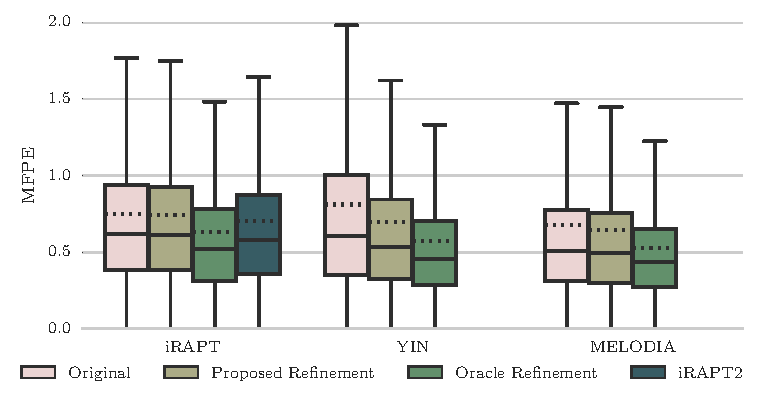
\includegraphics[width=0.90\columnwidth]{Chapters/05_Separation_Known/figures/stats_boxplot_ptdb_real.pdf}
\caption{Results from the real recordings PTDB-TUG dataset. MFPE grouped by estimator. Solid/dotted lines represent medians/means. Outliers are not shown.}
\label{fig:ptdbtug_real}
\end{figure}

\begin{figure}[t]
\centering
		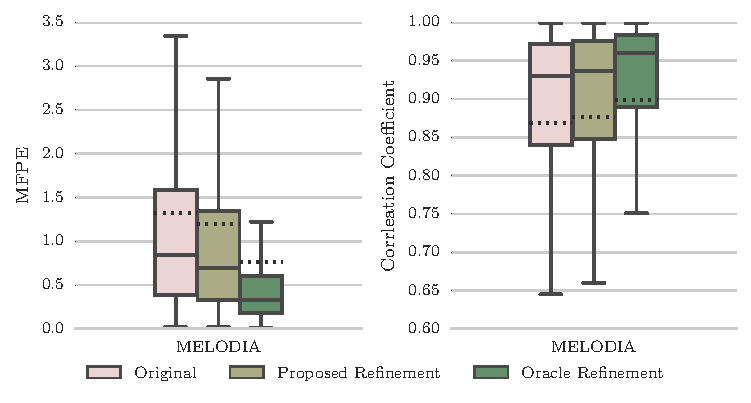
\includegraphics[width=0.90\columnwidth]{Chapters/05_Separation_Known/figures/stats_boxplot_medley.pdf}
\caption{Results from the real recordings MedleyDB dataset. MFPE and Correlation Coefficient grouped by estimator. Solid/dotted lines represent medians/means. Outliers are not shown.}
\label{fig:medley}
\end{figure}

\section{Summary and Discussion}

% start zafar
While methods focusing on harmonic models for the lead often fall short in their expressive power for the accompaniment, the methods we reviewed in this section are often observed to suffer exactly from the converse weakness, namely they do not provide an adequate model for the lead signal. Hence, the separated vocals often will feature interference from unpredictable parts from the accompaniment, such as some percussion or effects which occur infrequently.

Furthermore, even if the musical accompaniment will exhibit more redundancy, the vocals part will also be redundant to some extent, which is poorly handled by these methods. When the lead signal is not vocals but played by some lead instrument, its redundancy is even more pronounced, because the notes it plays lie in a reduced set of fundamental frequencies. Consequently, such methods would include the redundant parts of the lead within the accompaniment estimate, for example, a steady humming by a vocalist.
% end zafar

Future work could include a robust multi pitch variation estimator for musical instruments. Salamon and Gomez~\cite{salamon12} describe the current state of the art of f0 estimation. Some approaches use source separation to estimate multiple f0 pitch tracks. Therefore our approach shows that a robust multi pitch f0 estimate can also help to improve source separation. In the future an iterative multi-step procedure could lead to better results in both problem domains.\par

% from DAFX conclusion

This paper proposes a new source separation scenario for instruments played in unison. It highlights the time-varying aspects of the signal sources like amplitude or frequency modulations. By addressing these aspects, the separation quality for non-unison mixtures can generally be improved, too.
Furthermore we present two methods to decompose those mixtures based on differences in the amplitude or frequency modulation of the sources. One is using a method already published based on a modulation tensor factorization. The other is a novel method that uses an estimate of the pitch variation of the two input sources to warp the mixture. Within the warped domain the frequency modulation of the desired source is removed so that the sources can be separated more easily from the mixture. The results of 45 mixtures have been evaluated by using the PEASS toolbox. The scores indicate an improvement in favor of the pitch variation informed NMF compared to the standard NMF.

* Warping based separation is simple and can work surprisingly well on some signals but is generally of limited use.
However, the presented concepts such as warping are transferrable...

* Fundamental concepts stay the same for ML models. 
* End-to-End source separation does exist, but 
* DNN based (superior) melody estimation
* Modulations CTC (warped) loss functions.
* Applications for Style transfer (applying modulation characteristics on other voices or instruments)
* Generative Models for modulations (generate artificial vibrato)

